%%
%% This is file `ddis_thesis-EN.tex'
%% Change log
%%
%% 20.10.05 initial version                 Christoph Kiefer (ck)
%% 13.12.05 textwidth enlarged              ck
%% 15.05.06 caption error removed           ck
%%          README update
%% 18.05.08 added apalike_brackets package  ck
%%         (thanks to Andreas Bossard)
%%

%==============================================================================
% Prolog
%==============================================================================

\documentclass{ddis-thesis-EN}
% Include AMS extension for formulas
\usepackage{amssymb}

% Use PostScript fonts instead of LaTeX bitmap fonts (better for PDF)
\renewcommand{\rmdefault}{ppl}
% use Frutiger font
\renewcommand{\sfdefault}{pfr}
\renewcommand{\ttdefault}{pcr}

% Use advanced graphics inclusion and caption styles
\usepackage[pdftex]{  hyperref,bookmark,graphicx} 
\usepackage{epstopdf}

\usepackage{caption}
\renewcommand{\captionlabelfont}{\sffamily\bfseries}
\renewcommand{\captionfont}{\sffamily}

% Use subfigure and change the numbering style for subfigures
\usepackage{subfigure}
\renewcommand{\thesubfigure}{\alph{subfigure}}
\makeatletter
\renewcommand{\@thesubfigure}{(\thesubfigure)\space}
\renewcommand{\p@subfigure}{\thefigure}
\makeatother

% Use color package and define background and frame color for text boxes
\usepackage[pdftex]{color}
% Use label replacement for postscript figures
\usepackage{psfrag}
% Use Changebar
\usepackage{changebar}
% Use url
\usepackage{url}
% Use longtable environment
\usepackage{longtable}
% break citations
\usepackage{apalike_brackets}
% include TOC extensions for all Indexes
\usepackage{tocbibind}
% Redefine the headers with the fancyhdr package
\usepackage{fancyhdr}
\pagestyle{fancy}
\renewcommand{\chaptermark}[1]{\markboth{\chaptername \ \thechapter.\ #1}{}}
\renewcommand{\sectionmark}[1]{\markright{\thesection\ #1}}
\fancyhf{}
\fancyhead[LE,RO]{{\sffamily{\bfseries\thepage}}}
\fancyhead[LO]{{\sffamily{\rightmark}}}
\fancyhead[RE]{{\sffamily{\leftmark}}}
\renewcommand{\headrulewidth}{0.5pt}
\renewcommand{\footrulewidth}{0pt}
\addtolength{\headheight}{0.5pt}
\fancypagestyle{plain}{
  \fancyhead{}
  \renewcommand{\headrulewidth}{0pt}
}

%configure listings package
\lstset{ captionpos=b}

% Clear Header Style on the Last Empty Odd pages
\makeatletter
\def\cleardoublepage{\clearpage\if@twoside \ifodd\c@page\else%
    \hbox{}%
    \thispagestyle{empty}%              % Empty header styles
    \newpage%
    \if@twocolumn\hbox{}\newpage\fi\fi\fi}
\makeatother

\setlength\textwidth{15cm}
\setlength\oddsidemargin{3.5cm}
\setlength\evensidemargin{2.5cm}

\renewcommand\bibname{Bibliography}

%==============================================================================
% Begin of document
%==============================================================================

\begin{document}

\frontmatter

\begin{titlepage}

\setlength{\textwidth}{16cm}
\setlength{\oddsidemargin}{0cm}
\setlength{\evensidemargin}{0cm}
\setlength{\topmargin}{8mm}
\setlength{\headheight}{0cm}
\setlength{\headsep}{0cm}
\setlength{\topskip}{0cm}
\enlargethispage{5cm}

\noindent
\setlength{\unitlength}{1mm}
\begin{picture}(160,226)
\centering

\put(0,203){\line(1,0){160}} % lower line
\put(109,39){\line(1,0){50}}
\put(109,161){\line(1,0){50}}
\put(109,170){\line(1,0){50}}
\put(107,1){\line(0,1){200}}

\put(0,140){\parbox[b]{100mm}{
    \begin{center}
    {\bf\Huge {\sffamily{Building an adapting Poker Agent }}}
    \end{center}}}

\put(10,20){{\centering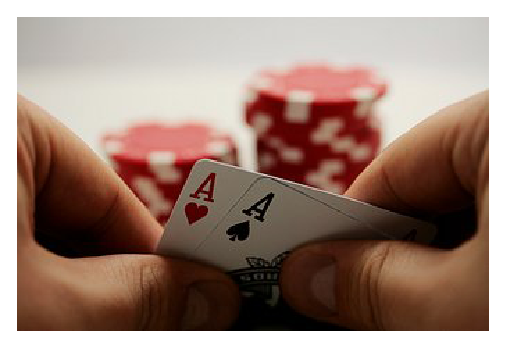
\includegraphics[width=8cm]{section-title/figures/poker}}}

\put(109,92){\parbox[b]{50mm}{
    {\bf
    {\sffamily{{\Large Christian K\"undig}}}}\\
    {\sffamily{of Z\"urich, Switzerland\\\\
    Student-ID: 04-706-743\\
   ch.kuendig@kuendig.ch
    }}
}}

\put(109,161){\makebox(50,9){{\sffamily{Master Thesis\hfill\today}}}}

\put(0,215){\makebox(80,11)[l]{
\includegraphics[height=2.8cm]
{section-title/figures/logo-ifi-e}}}

\put(109,184){\makebox(50,9)[t]{\centering\includegraphics[width=4.75cm]
{section-title/figures/ddis_txt}}}

\put(109,32){\parbox[b]{50mm}{\flushleft
    {\sffamily{Advisor:}} {\bf {\sffamily{Prof. Abraham Bernstein}} }
    }
}

\put(109,10){\parbox[b]{50mm}{\flushleft
        {\sffamily{
        Prof. Abraham Bernstein, PhD\\
        Department of Informatics\\
        University of Zurich\\
        http://www.ifi.uzh.ch/ddis}
        }
}}

\end{picture}
\end{titlepage}


\setlength{\hoffset}{-1in}

\fancyheadoffset[RO,LE]{2.5cm}
\fancyhfoffset{0in}

\begin{acknowledgements}

I would like to thank everyone that contributed to this thesis, namely:

\begin{itemize}
\item \textbf{Lukas Messmer} for playing the final implementation giving invaluable comments and judgment. 
\item \textbf{Janne Kyt\"om\"aki} for providing me with his wrapper for the PokerAcademy and the pokerserver API. The folks at the Pentaho, pokerai.org and Computer Poker Competition Forums.
\item \textbf{Prof. Bernstein} for giving me the freedom to pursue a thesis outside his usual field of research.
\item Last but not least, all of family and friends who kept asking for progress on a daily basis, both in pressuring and encouraging fashion.

 
\end{itemize}\end{acknowledgements}

\begin{abstract}
Poker offers an interesting domain to investigate some fundamental problems in artificial intelligence. The properties of stochasticity and imperfect information pose new challenging questions, not present in other typical game research subjects like chess; traditional methods for computer game-playing as alpha-beta search are incapable of handling these challenges.

This thesis presents the necessary algorithms to tackle these problems with the use of modified game tree search and opponent modeling. A proof-of-concept implementation for the game of No-Limit Texas Hold'em is provided (and benchmarked), based on the Miximax algorithm and an opponent model implemented as a Hoeffding tree. 
\end{abstract}

\begin{zusammenfassung}
Das Kartenspiel Poker bietet eine neue, interessante Umgebung um Problemstellungen der k\"unstlichen Intelligenz zu erforschen. Imperfekte Information und der Zufallsfaktor welche dem Spiel inne liegt, fehlen in anderen bereits ausgiebig erforschten Spielen wie Schach, weswegen traditionelle Vorgehensweise wie die alpha-beta Suche f\"ur diese neuen Herausforderungen kaum wiederverwentet werden k�nnen.

Diese Masterarbeit besch\"aftigt sich ausf\"uhrlich mit den n\"otigen Algorithmen um das Pokerspiel mit neuen Suchb\"aumen und Gegenermodellen zu bew\"altigen. Die Implementation eines m\"oglichen Vorgehens mit dem Miximax Algorithmus und einem Gegenermodel basierend auf Hoeffding Trees wird vorgestellt, und anderen Ans\"atzen in einem Benchmark-Turnier gegen\"ubergestellt.
\end{zusammenfassung}


\tableofcontents

\mainmatter

% arabic numbering after this
\pagenumbering{arabic}

\chapter{Introduction}

Game playing always presented an attractive tasks for artificial intelligence research. Already in the early 1950ies, in the wake of the first programmable computers, games have drawn the attention of researchers. Chess had been tackled by early computer scientists like Konrad Zuse, Claude Shannon (the inventor of information theory), Norbert Wiener (the creator of modern control theory) or Alan Turing \cite{Friedel2002}.

Also in the fifties, the first academic research of poker was conducted. Since computers were still way to slow to provide any assistance to analyze a full fledged poker game, \cite{Kuhn1950}�invented his own simple version of poker. For this very simple version, consisting only of a deck of three cards, two players with one hole card each, one betting stage and no community cards, Kuhn was able to calculate a complete equilibrium solution. He demonstrated that there are many game theoretic optimal strategies for the first player in this game, but only one for the second player, and that, when played optimally, the first player should expect to lose at a rate of $-\frac{1}{18}$ per hand. 

Since then, there has been steady progress in the standard of play strength of artificial intelligent algorithms, to the point that machines have surpassed humans in Checkers and Othello, have defeated human champions in Chess and Backgammon, and are competitive in many other games. Few exceptions remain, one being Go, where computers notoriously perform weak, and poker, where tremendous progress has been made in the last decade, but a wealth of unsolved problems still remain.

As \cite{Russell2003} mentions, game are interesting because they often are too hard to solve. Chess has an average branching factor of about 35, with games often going to 50 moves per player, so the search tree has about $35^100$ (or $10^154$) nodes. 
Games, like the real world, therefore require the ability to make some decision even when calculating the optimal decision is infeasible. Games also penalize inefficiency severely. Whereas an implementation of a algorithm is half as efficient will simply cost twice as much to run to completion, a game program that is half as efficient in using its available time probably will be beaten into the ground.

In poker, the actual game tree does not branch as much as in chess, but the addition of chance imperfect information pose challenges of similar amplitude. Kuhn Poker remains one of the few simple examples, where a complete solution has been found, with even simple (compared to other poker variants) variants like Heads-Up Limit Texas Hold'em still remaining a challenge.

\section{About Poker}
Poker is a well-known card game which gained a lot of popularity in the last years, thanks to plenty of online sites, offering to play the game online with real cash. 

Poker proceeds in stages, in each stage, cards are dealt (some of which are dealt face down only for one player to see and some of which are dealt face up for all players to see).  Players then wager against each other that their hand of cards is the best, or will be the best when the hand is played to the end. 

To remain active in the game, and keep a chance to win all the wagered chips, a player must match the amount of money bet by each of their opponents. If one player makes a bet that no opponent matches, then the game ends immediately with that player winning the game and all the bets placed and matched so far (the pot) - regardless of the cards they actually had. In the other case, if all bets are matched, play continues into the next stage, until there are no stages left in the game, and all active players reveal their cards in a showdown. The player with the highest ranked hand at that point then wins the pot.

Because each player only knows their own cards, and the common board cards, but lacks information about their opponents' hole cards, poker is an example of a domain of imperfect information.

While for most of the last century limit poker was popular, the focus of a lot of players has shifted to No-Limit variations of the game. Unlike with limit poker, in No-Limit Poker the possible wagers a player can do are only limited by the amount of chips he owns. This thesis will mainly focus on the No-Limit variant.



\chapter{Motivation}
\begin{verse}
Perhaps chess is the wrong game for the times. Poker is now everywhere, as amateurs dream of winning millions and being on television for playing a card game whose complexities can be detailed on a single piece of paper. But while chess is a 100 percent information game - both players are aware of all the data all the time- and therefore directly susceptible to computing power, poker has hidden cards and variable stakes, creating critical roles for chance, bluffing, and risk management.

These might seem to be aspects of poker based entirely on human psychology and therefore invulnerable to computer incursion. A machine can trivially calculate the odds of every hand, but what to make of an opponent with poor odds making a large bet? 
\end{verse}
\textit{The Chess Master and the Computer} by Garry Kasparov, 2009

\section{Poker and A.I. Research}
Poker is a complex game involving uncertainty, chance and the requirement for strategic and game-theoretic reasoning. Playing this game well, requires the use of intricate strategies as well as a fond knowledge of the stochastic foundations of the game. 

Novice players might see poker as a pure game of chance and look for strategies that play each hand according to its chance of being the best hand in play. This completely misses the fact that the presence of imperfect information allow the usage of advanced strategies, to hide and misrepresent information about a players own card, and trying to win a pot without holding the strongest hand.

The two features of stochasticity and imperfect information have made poker an interesting field for A.I. research. Thanks to a recent boom of poker and computer poker research as well, regular computer poker competitions ( \cite{TheAnualComputerPokerCompetition2010} and  human-computer matches (\cite{TheFirstManMachinePokerChampionship2007},\cite{TheSecondManMachinePokerCompetition2008}) are conduected.

There has been a recent flurry of research into developing strong programs for playing poker. Just as chess was once seen as an important challenge problem for AI, poker is now starting to be seen in the same way. Research has progressed to a point where Heads-Up Limit Hold'em programs have shown performances capable of winning against some of the best professional poker players. 

Thanks to various characteristics, poker is a appropriate testbed to apply concepts of artificial intelligence. The most important ones, according to \cite{Schauenberg2006} thereby are: 

\begin{itemize}
	\item \textit{decision-theory and probabilistic reasoning} - The randomness from the deal of cards and the lack of knowledge of the opponents cards make poker a noisy and uncertain domain. This forces a player to be adept at both decision-theory and probabilistic reasoning.
\item  \textit{risk assessment} - Poker is played in stages containing both the deal of additional cards and wagering. To be able to handle this type of domain of chance, a successful player must be able to assess risks.
\item \textit{opponent modeling} - In poker each hand represents a repeated against the same adaptive agent. This type of environment allows a player to use opponent modeling to
learn their opponents playing strategies and attempt to exploit this knowledge to increase their profit.
\end{itemize}

Most of these aspects can also be found in other fields of artificial intelligence, with the chance of carrying over insights gained by computer poke into other realms, such as: 


\begin{itemize}
\item \textit{user modeling} - Opponent modeling is a form of user modeling. As such, its a recurring problem of modern A.I. research.

In typical user modeling research, a observer tries to find patterns in the behavior of an observed entity. The identified patterns can then be used to customize an application to take advantage of the identified user preferences.

\item \textit{policy-making or negotiation agents} - Game theorists long ago realized poker could be used to illustrate fundamental principles of game theory that have subsequently been applied to a variety of fields including law, politics and economics. 

The development of automated decision-making in poker could lead to advancements in creating tools for use in these domains.
\end{itemize}

The bulk of the research into computer poker, including that from the University of Alberta - currently one of the driving forces in this field, has been on Heads-Up Limit Texas Hold'em. In this game, the players only ever have at most three possible actions (fold, call, or raise). In No-Limit Texas Hold'em on the other hand, players may bet any amount up to the amount of chips remaining in their stack. This rule change significantly alters the optimal strategies, and also poses new research problems when developing a computer program for playing the game. 

For this reason and the fact that No-Limit Poker has become much more popular in the last few years his thesis will focus on the No-Limit variant - though most approaches can also be and have been used in Limit Poker.

\section{Texas Hold'em Poker Rules}
\subsection{Betting structures}

Texas Hold'em is normally played with small and big blinds and the possibility for antes. These forced contributions by the players next to dealer (blinds) or everyone (antes) provide a starting pot to win. 

A dealer button is used to represent the player in the dealer position; the dealer button rotates clockwise after each hand, changing the position of the dealer and blinds. The small blind is posted by the player to the left of the dealer and is usually equal to half of the big blind. The big blind, posted by the player to the left of the small blind, is equal to the minimum bet. In tournament poker, the blind/ante structure periodically increases as the tournament progresses, so players are forced to amass more and more chips to stay in the tournament.

When only playing with two players, e.g. at the end of a tournament, special 'heads-up' rules are enforced and the blinds are posted differently. In this case, the person with the dealer button posts the small blind, while the other player off the button places the big blind. Since the big blind has option, the dealer acts first before the flop. After the flop, the dealer acts last (as normal) and continues to do so for the remainder of the hand.

There�s no one rule of how to set up the betting in all games of poker. The four most common various of Texas Hold'em are limit, spread limit, pot limit and no limit.

\begin{itemize}
\item \textit{Limit} Hold'em has historically been the most popular form of Hold'em found in casino live action games in the United States. In limit Hold'em, bets and raises during the first two rounds of betting (pre-flop and flop) must be equal to the big blind; this amount is called the small bet. In the next two rounds of betting (turn and river), bets and raises must be equal to twice the big blind; this amount is called the big bet. 
\item \textit{Spread limit} is often played in home games. In a spread-limit game, a player can bet any amount within some range � for instance \$1-\$5. This results in a game where the minimum any player can bet is \$1, and the most anyone can bet or raise at one time is \$5. If someone wishes to re-raise, they must raise at least the amount of the previous raise. This minimal raise rule also holds true for pot-limit and no-limit.
\item In \textit{pot-limit} Hold'em, the maximum raise is the current size of the pot (including the amount needed to call). Other then that, all bets and raises are allowed.
\item \textit{No-Limit} Hold'em is the form most commonly found in tournament poker and is currently probably the most popular variant. In No-Limit Hold'em, players may bet or raise any amount over the minimum raise up to all of the chips the player has at the table (called an all-in bet). The initial minimum raise is equal to the big blind. 
\end{itemize}

\subsection{Play of the hand}

At the begin of each hand of Texas Hold'em, all players are dealt two cards face down, starting with the player left of the dealer (the small blind). Texas Hold'em is played with a standard 52-card deck containing no jokers. The two hidden cards are called the players hole cards. They are the only cards each player receives individually and they will only be revealed if a showdown occurs or a player shows them voluntarily after finishing the hand. 

The game begins with a pre-flop betting round, beginning with the player left of the big blind and continuing clockwise. In a betting round, each player is asked to act, either checking (passing on the action, if no call is required),  betting (placing a wager), calling (even another players bet) or raise (call a bet, and further bet an additional amount).

 A round of betting continues until every player has folded, put in all of their chips, or matched the amount put in by all other active players. The blinds are considered "live" in the pre-flop betting round, meaning that they contribute to the amount that the blind player must contribute, and that, if all players call around to the player in the big blind position, that player may either check or raise (or call/fold).

After the pre-flop betting round, assuming there remain at least two players taking part in the hand, the dealer deals a flop, three face-up community cards. The flop is followed by a second betting round. This and all subsequent betting rounds begin with the player to the dealer's left and continue clockwise.

After the flop betting round ends, a single community card (called the turn or fourth street) is dealt, followed by a third betting round. A final single community card (called the river or fifth street) is then dealt, followed by a fourth betting round. If at this point of the game, more than one players remain, each shows his hands (or mucks, if he surrenders the pot) and the pot is awarded to the player with the strongest hand.

\subsection{The showdown}

If a player bets and all other players fold, then the remaining player is awarded the pot and is not required to show his hole cards. If two or more players remain after the final stage, a showdown occurs. On the showdown, each player plays the best poker hand they can make from the seven cards comprising his two hole cards and the five community cards. A player may use both of his own two hole cards, only one, or none at all, to form his final five-card hand. If a player decided to surrender the hand (since another player might already have shown a stronger hand) he can muck his hand without showing, losing any right to the pot.

If the best hand is shared by more than one player, then the pot is split equally among them, with any extra chips going to the first players after the button in clockwise order.

\section{Related Work}
\label{s:relatedwork}

There are various ways to tackle the problems posed by Poker. This section will summarize the most common approaches used in the past and present. The methods involving game tree search will be thoroughly explained in the next chapter. 

\subsection{Expert System}
In a heuristic-based approach to playing poker a rule-based expert system is used to make a poker betting decision. To make a decision, the expert system first abstracts a complicated game state into some simplified scenario that has one or more heuristics (e.g. opponent behavior, a players hole cards and/or the public board texture) associated with it and then it uses that heuristic information to make a decision.

A heuristic based approach is appealing for novices of the game since it's possible to formulate simple rules to base ones play upon. There is a plethora of poker literature focusing on this approach by explaining the heuristics a player should spend attention to, and how to react to common game scenarios given these heuristics. Examples of this approach are hand-ranges to play or fold in the pre-flop stage or strategies to disguise ones hand. As these rule sets are inherently easy to reuse, they offer a natural starting point for building poker-playing programs. 

There are different ways to compile the heuristics which govern these betting strategies. As mentioned, they could be compiled by a domain expert (e.g. a professional poker player or book author), or another way would be to derive and refine computationally through trial and error. Like most rule-based artificial intelligence algorithms, these rule-sets unfortunately quickly become too large to further develop and test. This also holds true for poker, where a situation rarely occurs twice - and the required style of play can differ a lot between different opponents, so it's hard to find rules covering all possibilities that might occur during a game.

Nevertheless, due to the perceived simplicity, this approach was used for various implementations of poker-playing program. As reported, \cite{Waterman1970} attempted to learn production rules to define a betting system for 5-card draw poker. His program reportedly achieved roughly the level of play of an experienced human player. \cite{Smith1983} later revisited the same problem and achieved comparable performance in 5-card draw poker, despite using less domain knowledge. It has to be mentioned though, that 5-card Draw, quite popular at that time, is not as strategically complex as other poker games, like Texas Hold'em (\cite{Sklansky1999}).

\cite{Korb1999} created a computer player for heads-up 5-card stud poker. His player used a Bayes' Network to provide an heuristic betting strategy, enriched with opponent information to provide a better estimate of the winning chance of a hand. This player won against two simplistic test opponents, but lost against an amateur poker player.

The University of Alberta Poker Research Group, a strong driver of computer research, also developed two heuristic-based programs. In these two programs called Loki (\cite{Papp1998} and \cite{Davidson2002}), opponent modeling information was used to increase the accuracy of the computed hand strength and hand potential values on which their their expert-defined formula-based betting strategy based its strategy. These programs have shown an impressive performance in full-ring Texas Hold'em games. In the limit variance of the game they were crafted for, they achieved the level of an intermediate human player. 

Still, \cite{Davidson2002} concluded that these approaches won't scale to world-class play. They too believed that poker has to many different decision scenarios to be be sufficiently handled by any knowledge-engineered heuristic-based betting strategy. Another shortcoming was, that to debug such programs an poker expert was required to identify mistakes in the betting strategy and suggest the improvements necessary.

For this reasons, heuristic-based approaches have mostly been abandoned in academic research. The ease to build them though, makes them still popular for poker-teaching programs and poker bots used to (illegally) profit at low stakes on online poker sites (e.g. \cite{Devlin2008} and \cite{Bornert2009}). 

Poki still remains one of the best ring table players, mostly because research focus has shifted to heads-up poker.

\subsection{Simulation-Based Approaches}
\label{section:simulationbased}

Before the game tree algorithms described in the next chapters were developed, \cite{Billings1999} and \cite{Davidson2002} tried out another way, similar to the game tree search approaches to other game playing problems like chess.  Since game-tree search works so well in these domains, the natural step was to test something analogous to game-tree search in the poker domain.

Game-tree search will be further explained in chapter \ref{c:game-tree-search}. Put short, in most two-player perfect information games it has shown to be effective to search the extensive form of  game-tree several moves ahead, and then call an evaluation function. Unfortunately, in poker the best response for the opponent is unknown because we do not know what cards they are holding. 

Simulation based approaches choose among actions at a certain point of game, and try to simulate the rest of the game to figure out the payout of a certain action. Figure \ref{fig:simulation-vs-search} shows the difference between standard game-tree search algorithms with an evaluation method like alpha-beta (left) and a simulation with selective sampling (right). Unlike alpha-beta, where a full-breadth, but only limited depth search is conducted, simulations search a selection of paths to the leaf nodes of the tree. A technique known as Selective Sampling was used to assign probable values to the unknown variables (the cards of the opponents). Instead of doing a comprehensive but shallow search, a deep but sparse simulation can probe numerous times to the leaves. Each trial of the simulation selectively samples the search space. With enough trials the cumulative selective sample converges to a statistically confident result.

\begin{figure}[!ht]
\centering
\includegraphics[width=\linewidth]{section02-motivation/figures/simulation-vs-search}
\caption{The difference between classic game-tree search (left) and simulations (right). (\cite{Davidson2002})}
\label{fig:simulation-vs-search}
\end{figure}

In simulation-based Poki by \cite{Davidson2002}, each possible action was simulated by iterating he game to the end of the hand. Since the complete game-state is unknown, probably cards are assigned to each player in each trial of the simulation. After simulating hundreds of trials, an average amount won or lost is known for each action. The action with the largest expected value will then be played by Poki.

The betting strategy according to \cite{Davidson2002} determines the expected values as follows: 

\begin{itemize}
	\item For each trial, probably hands are assigned to each opponent to hold. They also choose hands for players that have already folded, to remove these cards from the deck. For each opponent, a card weight table is maintained throughout the game.
	\item Once each player has a simulated hand assigned, the unknown board cards are randomly chosen from the remaining cards in the deck.
	\item For each trial, the hand is simulated twice. In the first simulation, Poki first calls or checks, in the second Poki would raise of bet (obviously, Poki was used to play limit poker). Once the first action is made, the rest of the hand is simulated to completion. When a simulated opponent must act, their opponent model predicts what he would most likely do in that context. 
	\item Once the simulated hand is finished, the net amount won or lost is recorded.
\end{itemize}

\cite{Davidson2002} reports that in the limited time frame of one or two seconds, around 200-300 trials can be simulated. After this number of trials, the average EV for the different action must have become reasonably stable.

The biggest benefit over rule-based systems outlined before, is that complex strategies can be uncovered without any specific expert knowledge. Tactics such as check-raising, slow playing and bluffing are an emergent property of the simulations. 

Unfortunately, this approach still did not perform as well as hoped. While in ring games, Poki was competitive with intermediate human players, in heads-up games if even lost to very moderate humans. The main reason Poki's simulations did not perform as well as hoped was mostly attributed to the method being extremely dependent on the correct prediction of the opponents future play. Deciding on a single opponent action is extremely difficult, if not impossible, since most opponents also adapt to the situation of the game, and rather think of a distribution of actions to play. By branching at each possible opponent action, the search approach later explained in chapter \ref{c:game-tree-search} takes this into consideration  


\subsection{Game-Theoretic Approaches}
In Game Theory, a nash equilibrium describes a solution of a game, where all players have nothing to gain by changing their own strategy. There can be several different (and possibly infinitely many) equilibria for any given game, but if the game is two-player and zero-sum, every Nash equilibrium provides the same payoffs to all players. In a repeated game where the players change positions, such as heads-up poker, this is a very useful feature - if both players are playing an equilibrium strategy, the expected score for both players will be zero. If one player plays the equilibrium strategy, since their opponent cannot do better by playing a strategy other than the equilibrium, they can expect to at least tie the game.

Unfortunately, due to the complexity of poker (and most other real world games), a equilibrium strategy is rarely achievable. Instead, an approximation of the equilibrium is searched and played - called an  $\epsilon$-Nash equilibrium strategy.  $\epsilon$ is the measure of how far from the actual equilibrium the strategy is. Since a pure equilibrium strategy would loose nor gain more than 0 against any opponent,  $\epsilon$ is the value a best response could win against an  $\epsilon$-equilibrium strategy. Therefore,  $\epsilon$-equilibrium strategies are called suboptimal, or exploitable. But as long as the abstraction is strategically similar to the real game, these strategies can be very difficult to defeat in the full game.

As there are various general-purpose algorithms to calculate equilibria with linear equations, there exist various approaches towards creating $\epsilon$-Nash equilibria agents for poker.

A game theoretic approach results in a approximation of what could be described as "solving" poker, since it searches a generally valid strategy offline, instead of specifically "deciding" what to do in a specific situation during the game. The game theoretic solutions are usually calculated before the game - this limits its ability to adapt to an opponent, but allows for very strong optimization.

\subsubsection{University of Alberta, Edmonton}

The Computer Poker Research Group at the University of Alberta has developed a variety of $\epsilon$-Nash equilibrium strategy agents.

To take the missing information into consideration, the University of Alberta uses a concept they call information sets. A information set contains all possible and indistinguishable states of an opponent in a game tree. All states in the game tree that only differ by the hand an opponent might hold, are therefore collected into one node - a information set. 

Strategies for extensive form games like poker can be represented in several ways. One straightforward way would be to enumerate all possible information sets and record the probabilities of taking each action from that information set.

An alternate method of representing a strategy is to store the probability of playing along each sequence of actions. Considering a sequence of actions by a player and its opponents that have reached a terminal state. Assuming that the player and the opponent play to reach this outcome, we can find the probability of the player selecting their actions in this sequence. This is known as a realization weight.

A set of such realization weights defines a strategy. To find action probabilities at an information set during a game, the sum of the realization weights associated with all reachable terminal nodes after this action can be summed up. 

A linear program can be created to find optimal realization weights subject to constraints (action probabilities are non-negative and sum up to 1). The result is a pair of strategies that are best responses to each other: a Nash equilibrium. 

The \textit{PsOpti} family of programs use an abstract version of the game, which then gets converted into the sequence form. The sequence form then is treated as a series of constraint in a linear program. A solver then can solve these equation system to find an $\epsilon$-Nash equilibrium strategy.

But even after such an abstraction, in the case of the \textit{PsOpti} family of programs, the program needed to solve the entire abstract game was too large to fit into the memory of a computer or a cluster of computers. 

To shrink it, so it could fit into a computers memory, two additional abstractions had to applied. For one thing, they changed the rules of Limit Hold'em so one less bet was allowed on each stage (only two bets or raises Pre-Flop and three on the other stages - \textit{PsOpti} was only playing Limit Hold'em).

Then, seven 3-round Flop strategies were created; each one assumes a different Pre-Flop betting sequence (check-call, check-bet-call, etc) was followed. This combination of strategies could then be used to compose the overall strategy. 

This Pre-Flop strategy was only used on the Pre-Flop. On the flop, a different post-flop strategy was computed and chosen, depending on the observed Pre-Flop action of the player and the opponent.

This disconnect between the Pre-Flop strategy and the strategy used in the rest of the game was a flaw in the \textit{PsOpti} agents that could be exploited by bots with a good opponent model, or by human players aware of this flaw. 

Later Agents tackled that problem by forming one cohesive strategy (\cite{Zinkevich2007b} ) for the whole game or a more robust  $\epsilon$-Nash equilibria approximation (\cite{Johanson2007}). Both approaches saw a immediate increase in performance over the previous \textit{PsOpti1-4} agents.

\textit{Smallbot2298} is another game theoretic approach from University of Alberta. It was produced by a method that does not directly involve solving a linear program, as with the \textit{PsOpti} family of programs and the \textit{GameShrink} approach from the Carnegy Melon University explained later on. Instead, it uses a algorithm described as "Range of Skill" by \cite{Zinkevich2007b}.  It was also one of the first $\epsilon$-Nash equilibrium strategy to use one consistent, whole-game strategy, as opposed to the overlapping strategies used for \textit{PsOpti} and the (first offsprings of the) \textit{GameShrink} family.

The basic idea behind Smallbot2298 is the creation of a sequence of agents, where each one can defeat the agents earlier in the sequence by at least $\epsilon$. For any game and a value for $\epsilon$, this sequence has a maximum length-  sooner or later the sequence approaches within $\epsilon$ of a Nash equilibrium, and no further agents are able to defeat it by more than $\epsilon$. 

To construct this sequence of agents, two algorithms are applied. The first algorithm, \textit{Generalized Best Response I}, considers a game where player 1 is restricted to a set of allowed strategies $S'_1$ while player 2's set $S'_2$ only contains one strategy. A nash equilibrium for this game $G = (S'_{1},S'_{2},u)$ is calculated and the best response for player 2 to player 1 s equilibrium strategy is deducted. This strategy is added to the set $S'_2$ and the algorithm starts again. After enough repetitions, player 2's half of the equilibrium is returned as the best response to player 1's set of strategies $S'_{1}$. 

The second and essential algorithm for this approach, \textit{Range of Skill}, repeatedly calls the generalized best response. After initializing a set of allowed strategies to contain an arbitraty strategy the generalized best response is used to calculate an equilibirum strategy for one player in the restricted game where the other player max only mix between the set of allowed (initially arbitrary) strategies.  This resulting strategy is capable of defeating any of the strategies in the set. 

\begin{lstlisting}[mathescape=true, caption=Algorithm 1: Double Oracle Bundle Algorithm \cite{Zinkevich2007b}]
1. Initialize $S' _1 \subseteq S_1$ and $S'_2 \subseteq S2$. These could be arbitrary singletons.
2. Repeat until satisfied.
2.a) Find a Nash equilibrium $(\sigma_1,\sigma_2)$ in the restricted game $G = (S'_1,S'_2,u)$.
2.b) Compute $BR(\sigma_1)$ and add it to $S'_2$. 
2.c) Compute $BR(\sigma_2)$ and add it to $S'_1$.
3. Return $(\sigma_1, \sigma_2)$.
\end{lstlisting}

\begin{lstlisting}[mathescape=true, caption=Algorithm 2: Generalized Best Response \cite{Zinkevich2007b}]
1. Given $S' _1 \subseteq S_1$, initialize $S' _2 \subseteq S_2$ arbitrarily. 
2. Repeat until satisfied.
2.a) Find a Nash equilibrium  $(\sigma_1,\sigma_2)$ to  $G = (S'_1,S'_2,u)$.
2.b) Compute  $BR(\sigma_1)$ and add it to $S'_2$.
3. Return $\sigma_2$.
\end{lstlisting}

\begin{lstlisting}[mathescape=true, caption=Algorithm 3: Range-Of-Skill Algorithm \cite{Zinkevich2007b}]
1. Initialize $\sum' \subseteq \Delta(S)$ as a singleton. 
2. Repeat until satisfied.
2.a) Find an $\epsilon'$-generalized best response to $\sum' \sigma$.
2.b) Add $\sigma$ to $\sum'$.
3. Return one of the safest mixed strategies $\sum'$ as an $\epsilon$-Nash equilibrium.
\end{lstlisting}

After adding that strategy to the set of allowed strategy, the generalized best response algorithm is called again. Each strategy returned by the generalized best response algorithm in this way is a member of the "range of skill", as each one is capable of defeating the strategies generated before it. The more the sequence of strategies grows, the more the most recent strategies at the end of the sequence approach a Nash equilibrium.

Memory requirements are both the main advantage and disadvantage of the Range of Skill algorithm. By limiting the players of the abstracted game to picking a fixed set of strategies, it avoids solving a huge linear program for the whole game. By circumventing that problem that has hindered other game theoretic approaches, it was possible to deviate on of the first full-game limit Hold'em strategies, without fragmenting like \textit{PsOpti} and \textit{GameShrink}.

On the other hand, for the Range of Skill algorithm, a huge amount of intermediate data has to be stored. Each intermediate strategy most be kept for use in future steps, e.g. to calculate the utility matrix. This data can be stored on a hard disk as opposed to in RAM (for a linear program), but must still be loaded and unloaded often. For scaling to larger abstractions, this might become a problem as \cite{Johanson2007} mentions.

Like other equilibrium approaches, \cite{Zinkevich2007b} ends on the conclusion that even though an equilibrium is a very safe strategy, its rarely the best (exploitive) strategy when playing against a weaker opponent. Game theoretic equilibrium strategies are always defensive strategies, often without the optimal balance between exploitation and safety.


\subsubsection{Carnegie Mellon University, Pittsburgh}

Gilpin and Sandholm from the Carnegie Mellon University produced various nash equilibrium approximations based on their Game Shrink family of algorithms (\cite{Gilpin2006,Gilpin2006b,Hoda2006,Gilpin2007,Gilpin2007b,Gilpin2008}). The resulting players have repeatedly shown to be competitive opponents in the Annual Computer Poker Competitions.

Although Gilpin and Sandholm use a different terminonoly, they share a common foundation with the \textit{PsOpti} agents of the University of Alberta. In their approach, a hand strength metric is called an ordered signal; instead of cards, the agent receives a signal whose value corresponds to the probability of winning the hand. Instead of the term "bucket" to abstract hands, they use the term information filter, which coarsens the ordered signal into a discrete value.

Both \textit{GS1} and \textit{GS2} compute a truncated $\epsilon$-Nash equilibrium strategy to use in the Pre-Flop and Flop rounds. For \textit{GS1}, this truncated strategy considers the betting and cards on the Pre-Flop and Flop rounds; \textit{GS2} considers the betting and cards on the Pre-Flop, Flop and Turn rounds. Both programs use terminal nodes after this point to represent the estimated outcome of the remaining rounds. GS3 and Tartarian later on focused on full-depth equilibrium (\cite{Gilpin2008}). To truncate the remaining stages in \textit{GS1}, they assume that both player call during the Turn and River rounds - resulting in a simple rollout of the later stages of the game. \textit{GS2} uses an estimate of the betting strategy used by \textit{PsOpti}4, conditioned only on the cards and not the earlier betting, as an estimate for the betting actions by both players on the River.

After the turn, the programs construct a linear program in real time and solve it to find a new equilibrium strategy to use later on. As the pre-flop, flop and turn cards are known, the linear program can use a precomputed abstraction that corresponds to the specific set of community cards. For speed, 135,408 of these precomputed abstractions are calculated offline. This provides a much more precise idea of the hand strength at this point in the game than the past filtered signals (buckets) could provide.

Assuming that the opponent is also playing according to the precomputed strategy, the hand strength can be estimated. The linear program to be solved can thus be designed for the current game state: it considers only the betting history that actually occured and the current  community cards.

This linear program is then solved in a separate process while the game further advances. If the player is asked for an action, the agent interrupts the linear program and an intermediate solution can be queried. 

While this allows the agent to produce actions on demand, there is a danger that, as the LP solution is further refined, this intermediate action is no longer part of the solution to the LP. This is called "falling off the tree" since the opponent played an action the strategy wouldn't have selected. The linear program is unable to suggest future actions after that action. In these cases, the agent simply calls for the remainder of the game. 

The main advantage of this approach is that, in theory, the equilibria strategy for the Turn and River rounds will be more accurate than an equilibria strategy in a normal bucket abstraction since the card information on the turn and river are much more precise.

Unfortunately, there are also several significant disadvantages of this approach. For one, solving the linear program in real-time is a difficult task. Normally, a decision has to be made in a matter of seconds (around one minute per hand in live poker, half of that in online poker and 7 seconds per average hand in the annual computer poker competition). In practice, even generating the linear program cannot be done quickly enough to be used in such a short time span.

Another disadvantage is the split between early game and late game. By assuming that both players will only call during the Turn and the River, the Pre-Flop and Flop strategies don't have a accurate estimation of the value of certain lines of player. The concept of implied odds is completely ignored this way.

Implied odds means, that if a strong hand that is likely to win, the amount of money to win isn't only the current pot, but the bets the opponent most call in future rounds. Since the Turn and River rounds have larger bet increments than the Pre-Flop and Flop, assuming that both players will simply call (as \textit{GS1} does) gives too little utility to strong hands, and too much utility to weak hands. 

Another disadvantage is the assumption that the opponent also plays the same equilibrium strategy as the agent. If the opponent does not follow the same Pre-Flop betting strategy as \textit{GS2} (and playing by a different strategy is very likely), then the linear program  used later in the game assumes an inaccurate strength for the opponents hand. And if the opponent doesn't follow the game tree in the turn and river stages, the linear program has lost all value whatsoever.

\chapter{Game Tree Search}
\label{c:game-tree-search}
In many games with relatively simple rules but deep strategy complexity, computer programs have surpassed the best human players by considerable margin. In most cases, the successful technique has been the same: building a search tree of the possible decisions, and evaluating the resulting game states with a domain-specific evaluation function - often accompanied by efficient alpha-beta pruning. Probably the most notable field for these successes are chess programs, like \textit{Deep Blue} which won a widely publicized exhibition match against then chess world champion Garry Kasparov in 1997. Since then, other programs like Fritz and Shredder achieved constant performances on par with or above the best human players, adding chess to the growing list of games dominated by computer programs (similar examples including Checkers and Othello are mentioned in \cite{Billings2006}).  

The approach has not been successful for the game of \textit{Go}, however, owing to the high branching factor and vast search space, and the fact that goals and sub-goals are very difficult to assess with heuristic evaluation.

This chapter will outline the strategies to solve game decision problems with search trees, and the required adaptations to use these algorithms in a non-deterministic and imperfect information game like poker.

\section{Deterministic games with perfect information}
\label{sec:perfectinformation}
Considering games with two players, \cite{Russell2003} explains the generic game tree search for deterministic, turn-taking, two-player, zero-sum games of perfect information. Although poker doesn't fulfill most of these attributes - cards are not dealt deterministic, ring-games can involve more than two-players and there is obviously no perfect information - the basic strategies outlined here can still be applied to find a solution on what action to take in a poker game - as shown in later chapters.

The basic game problem for this algorithm involves two player, called \texttt{MAX} and \texttt{MIN}, named after their strategic targets (\texttt{MAX} has to maximize payoffs, \texttt{MIN} tries to minimize them). \texttt{MAX} moves first, and then both player take alternating turns until the game is over. At the end of the game, the winning player gained something while the loosing player is punished (whatever the incentives are to win, respectively not to loose). A game can be formally defined as a search problem with these components (according to \cite{Russell2003}):

\begin{itemize}
	\item The \textbf{initial state}, which includes the board position and identifies the player to move.
	\item A \textbf{successor function}, which returns a list of \textit{(move, state)} pairs, each indicating a legal move and the resulting state.
	\item A \textbf{terminal test}, which determines when the game is over. States where the game has ended are called terminal states.
	\item A \textbf{utility function} (also called an objective function or payoff function), which gives a numeric value for the terminal states. In chess, the outcome is a win, loss, or draw, with values +1, -1, or 0. Some games have a wider variety of possible outcomes; the payoffs in backgammon range from +192 to -192. The payoffs in poker depend on the exact betting sequences leading to a terminal state.
\end{itemize}

In game theory, this representation is called the extensive form representation, opposed to the normal-form it allows easy analysis thanks to its tree-graph visualization of the game (\cite{Gilpin2007}).
 
Starting with the initial state as a node, with legal moves as links to resulting states (until a terminal state is reached), figure \ref{fig:tictactoe-tree1} shows part of a game tree for tic-tac-toe. From the initial state, \texttt{MAX} has nine possible moves. After those, the game alternates between \texttt{MAX} placing \texttt{X}s and \texttt{MIN} placing \texttt{O}s until a leaf node corresponding to a terminal state, where all fields are filled of one player has marked three fields in a row, is reached. The number on each leaf node indicates the utility value of the terminal state from the point of view of \texttt{MAX}; high values are assumed to be good for \texttt{MAX} and bad for \texttt{MIN}. The game tree is represented so that the best move for \texttt{MAX} has to be determined, as he is acting on the initial node.

\begin{figure}[!ht]
\centering
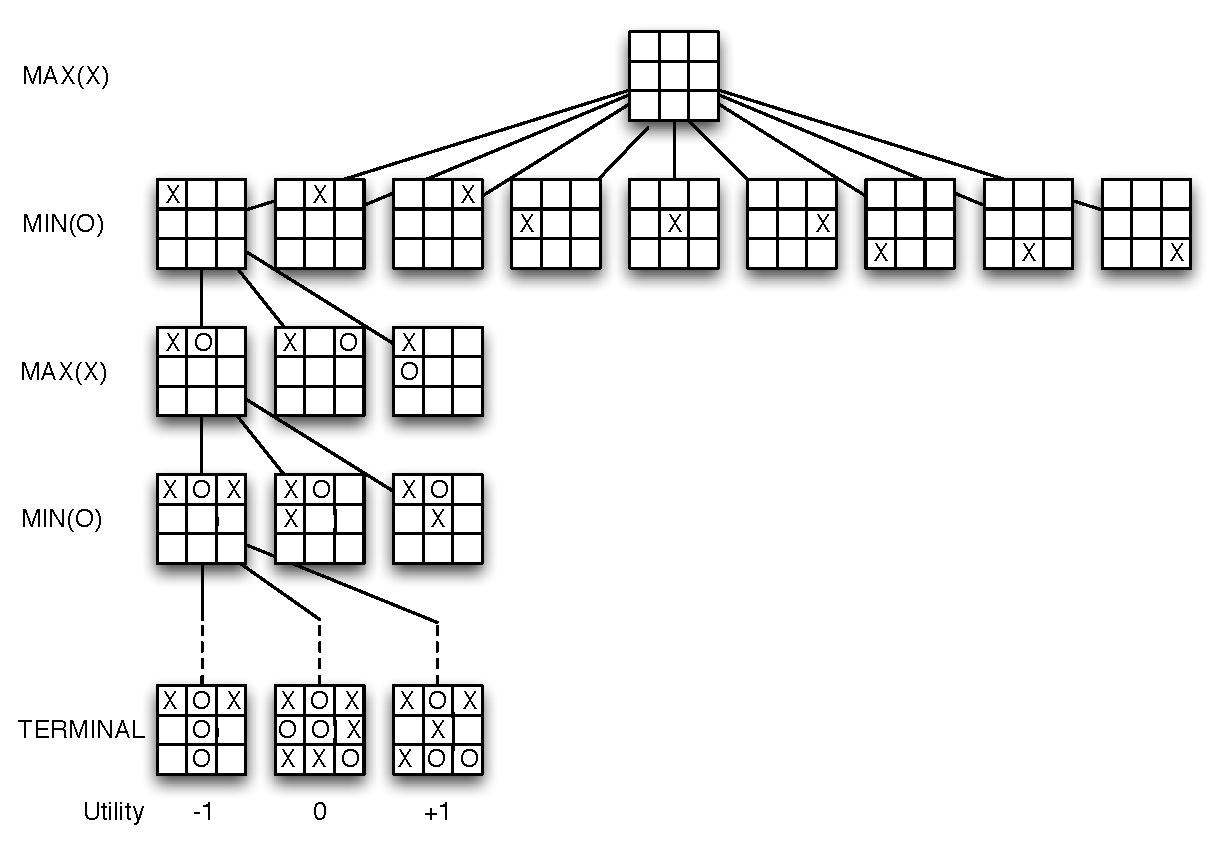
\includegraphics[width=\linewidth]{section03-gametree/figures/tictactoe-tree}
\caption{A partial search tree for the game of tic-tac-toe.}
\label{fig:tictactoe-tree1}
\end{figure}

\subsection{The Minimax Algorithm}
In a normal graph searching problem, the optimal solution would be a sequence of moves leading to a goal state with a high payoff (e.g. a win). In a game though, as \cite{Russell2003} explains, \texttt{MIN} obviously has the power to influence this sequence of moves. \texttt{MAX} must find a contingent strategy, which specifies a first move in the initial state, as well as the following moves in all states resulting from every possible response by \texttt{MIN} to those moves, until all such sequences end in a terminal node. As even tic-tac-toe is too complex to draw the entire game tree (not to speak of limit, or even no-limit poker), a much simpler game is presented in figure \ref{fig:trivialgame-tree}. Here, \texttt{MAX} is given three moves at the root node, labeled $a_1$, $a_2$ and $a_3$ to choose from. The possible replies by \texttt{MIN} are $b_1$, $b_2$ and $b_3$ if \texttt{MAX} chose $a_1$, $c_1$, $c_2$ and $c_3$ if \texttt{MAX} chose $a_2$ and the nodes designated with $d_n$ if \texttt{MAX} chose $a_3$. This game ends after one move by each player, resulting in a tree that is one move deep, consisting of two half-moves called \textit{ply}s. The payoffs vary in a range between 2 to 14.

\begin{figure}[!ht]
\centering
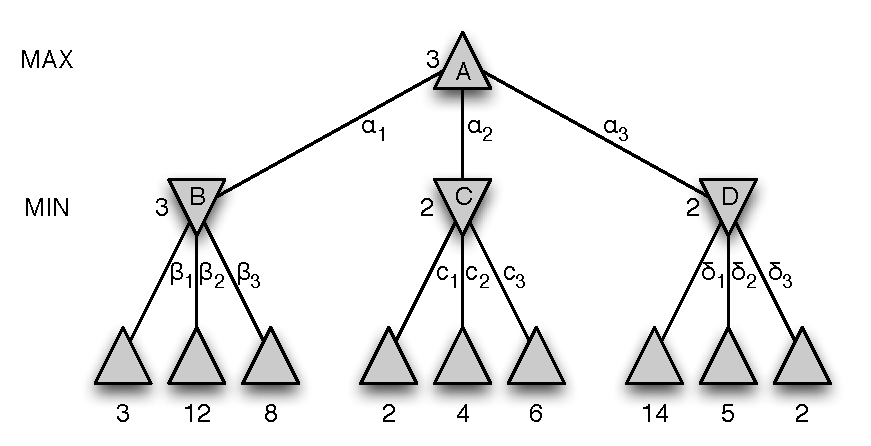
\includegraphics[width=\linewidth]{section03-gametree/figures/trivialgame-tree}
\caption{Game tree of the trivial game from \cite{Russell2003}. The $\bigtriangleup$ nodes are decision nodes of \texttt{MAX}, the $\bigtriangledown$ for \texttt{MIN}. The terminal nodes show the utility values for \texttt{MAX}.}
\label{fig:trivialgame-tree}
\end{figure}

After this game tree for the problem at hand has been created, the optimal strategy can be determined by examining the payoff of each non-terminal node, called the \textbf{minimax value}. Based on the premise that both player play optimal, the minimax value of a node is the utility (for \texttt{MAX}) of being in the corresponding state. Given a choice, \texttt{MAX} will prefer to move to a state of maximum value, whereas \texttt{MIN} prefers a state of minimum value. \cite{Russell2003} forms the following formula \ref{eq:minimax}: 

\begin{equation}
Minimax-Value(n) = 
 \left\{ \begin{array}{lll}
Utility(n) 															& \mbox{if n is a terminal state} \\
max_{s\in Successors(n)} Minimax-Value(s) & \mbox{if n is a MAX node} \\
min_{s\in Successors(n)} Minimax-Value(s) & \mbox{if n is a MIN node}
\end{array}
\right.
\label{eq:minimax}
\end{equation}

In figure \ref{fig:trivialgame-tree} the nodes are already marked with their minimax values. At the first \texttt{MIN} node, labeled $B$, \texttt{MIN} can choose between sucessors with values 3,12,8. As \texttt{MIN} tries to minimize the utility, $B$ gets the minimax value of 3. Analogue, the other two \texttt{MIN} nodes have a minimax value of 2. As the root node is a \texttt{MAX} node, the solution to this game problem will be the decision leading to the node with the highest minimax value: action $a_1$ with a expected payoff of 3. As \cite{Russell2003} mentions, this result assumes that \texttt{MIN} also plays optimally. This assumption only makes sense in deterministic games with perfect information. In this case, there may be other strategies against suboptimal opponents that do better than the minimax strategy; but these strategies necessarily do worse against optimal opponents. More about that will be outlined in section {sec:optimalvsmaximal} about situation where deviation from an optimal strategy is advantgeous or necessarily.

The minimax-algorithm uses a simple recursive computation, proceeding all the way down to the leaves, and then backing up the minimax values as the recursion unwinds. In figure \ref{fig:trivialgame-tree}, the algorithm first recurses down to the three bottomleft nodes, and uses the utility function on them to discover that their values are 3, 12, and
8 respectively. Then it takes the minimum of these values, 3, and returns it as the backed-up value of node B. A similar process gives the backed up values of 2 for C and 2 for D. Finally, we take the maximum of 3,2, and 2 to get the backed-up value of 3 for the root node. 

The minimax algorithm performs a complete depth-first exploration of the game tree. Unfortunately, for real games (and realtime calculations), the time cost for completely exploring the tree is often impractical. Nevertheless, this alogrithm serves as the basis for the mathematical analysis of games and for more practical, modified algorithms. These include the widly used alpha-beta pruning, adding a evaluation function instead of backing up the utility value or the modifications explained in the  following sections.

\section{Stochastic Games with imperfect information}
\label{c:imperfectinformation} 

Unlike Tic-Tac-Toe or the simplistic game used in figure \ref{fig:trivialgame-tree} many games (e.g. backgammon, monopoly etc.) include some element of random chance. The traditional game tree representation can be extended to include additional chance nodes which represent stochastic events and outcomes. Chance nodes spawn branches for each random outcome, with the same weight for each node (assuming the game uses a fair dice). 
From a search perspective, all of these branches must be considered, and combined to obtain an overall expected value (EV), so the size of the game tree grows multiplicatively with each subsequent chance node. As chance nodes don't maximize or minimize, the alpha beta pruning used in minimax-search is not directly applicable to this class of problems. But similar search algorithms such as *-Minimax \cite{Hauk2006} and Expectiminimax \cite[p. 175-180]{Russell2003} are able to handle this form of uncertainty adequately.

According to  \cite{Billings2006}, the property of stochasticity has not been a major	handicap for computer performance in practical games of chance, like backgammon. For backgammon, a game with perfect information, but a certain factor of chance (the roll of the dice) - artificial intelligence research has lead to excellent evaluation functions learned automatically from self-play (see \cite{Tesauro2002}), resulting in several programs that are at least on par with the best human players, without requiring deep search (see \cite{Hauk2006}) of the whole game tree.

But one major distinguishing factor between poker and other games which are subject to artificial intelligence research is the property of imperfect information. At first sight, it might seem that games of imperfect information are just like games with a probabilistic factor: the cards are dealt randomly and determine the moves available to each player, but all the dice are rolled at the beginning. In reality though, we can't just "roll" all possibly start-hands, calculate our actions and then average somehow. \cite{Russell2003} calls that "averaging over clairvoyance", and it can't be used to solve decision problems. The problem with this naive algorithm is that it assumes that in each possible deal, play will proceed as if all the cards are visible. In reality when information is missing, one must consider what information one will have at each point in the game. The following paragraphs outlines the algorithms currently used in computer poker and which are later applied in the implementation (chapter \ref{chap:implementation}). Other approaches to build a poker agent were summarized in section \ref{s:relatedwork}.

\subsection{Miximax Search}

Like perfect information games, games of imperfect information can be represented graphically as a tree. Nodes represent various states in the game, and edges connecting the nodes represent possible actions which cause a transition from one state/node to another. In an imperfect games, nodes have to be categorized into who is is choosing the action at that game state. In perfect information games, that isn't the case, as the optimal action (and its value) each player chooses can be perfectly deduced. Additionally, like in all games of chance, there are chance nodes, where a random process deals cards, and terminal nodes. 

\begin{figure}[!ht]
\centering
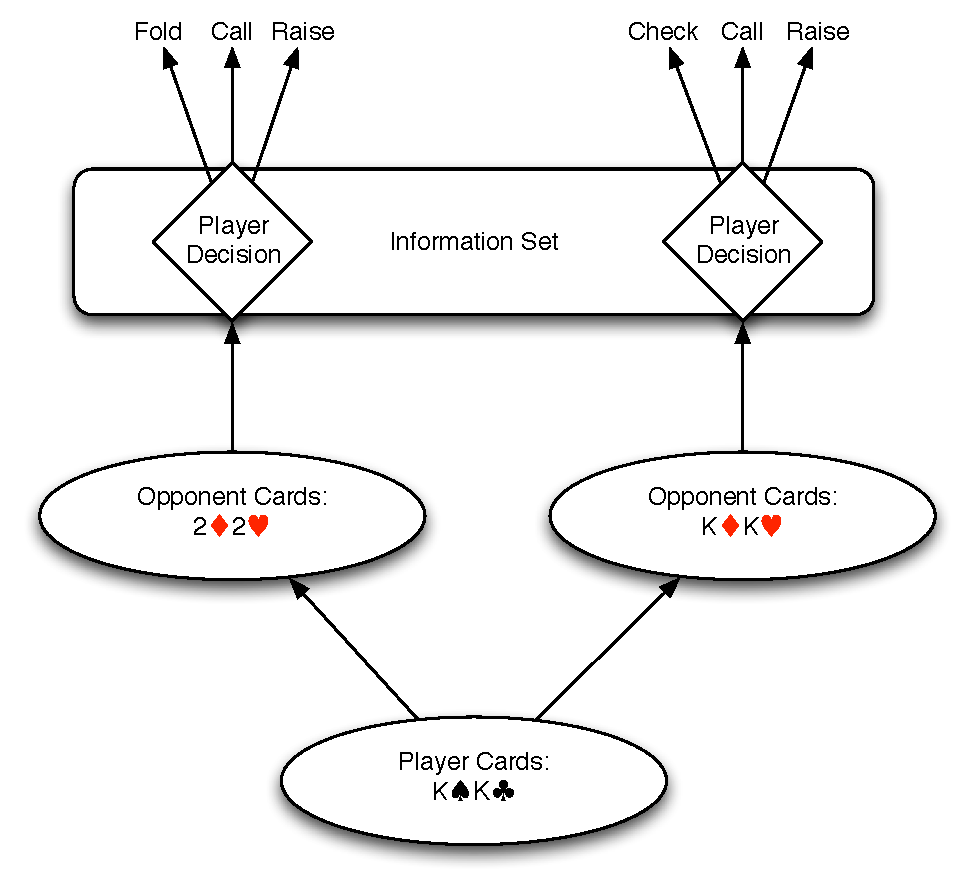
\includegraphics[width=\linewidth]{section03-gametree/figures/information-sets}
\caption{An example of a information set from \cite{Johanson2007}. For the player observing the opponent, its not possible to distinguish the two chance nodes that assign cards to the opponent. An information set contains these game stats that cannot be distinguished.}
\label{fig:information-sets}
\end{figure}

The presence of hidden information means, that the different action nodes of the opponent become indistinguishable, and the player is required to act the same way in all of them. A player can't calculate one action for when the opponent holds a pair, and another for the decision node where he does not hold one. He must find a solution which works in both situations. In game theory, all these action nodes belong to the same information set.  An information set is a set that, for a particular player, establishes all the possible moves that could have taken place in the game so far, given what that player has observed. This means that in Texas Hold'em, all of a player's action nodes that share both the same public information (i.e. the betting actions and community cards) and the same private information (i.e. the player's hole cards) but differ solely because of the opponent's private hidden information (i.e. the opponent's hole cards) belong to the same information set. In the extensive form representation of the game, an information set appears as an oval grouping together a set of player action nodes. (\cite{Schauenberg2006} )

To adapt the game-three for imperfect information games, \textit{information sets} are used. An information set is a set of decision nodes in the game tree that cannot be distinguished from the perspective of an observing player. Since the opponent's cards are hidden in poker, this corresponds to the complete set of all possible opponent holdings in a given situation. 

Obviously, the same strategy (such as a particular mixed strategy) must be applied identically to all of the nodes in the information set, as its obviously impossible to distinguish these states and adapt to them\cite{Billings2006}. 

As an consequence, nodes of the the same imperfect information tree are not independent \cite{Billings2006}.  Thus, a divide-and-conquer search algorithm, such
as the alpha-beta minimax technique explained in \cite{Russell2003}, is not applicable to this class of problems, since sub-trees (of the same information set) cannot be handled independently.

Figure \ref{fig:information-sets} shows an example of information sets. The two choice nodes of the player only vary by the opponents hole cards, and an information set contains these game states.  The player cannot tell if the if the opponent has the pair of twos or the pair of kings. During a game, only the information set the player is in is known - but not the particular game state within that information set.  Since we cannot tell the difference between the game states within the information set, any decision on how to act from that information set must be used for all game states within this set. In Figure \ref{fig:information-sets}, the player cannot decide to raise when the opponent has the pair of twos and call when he has the pair of kings. Since we cannot tell which state we are in, we must choose an action (or probability distribution over actions) to use when we encounter the information set - independent of the possible specific decision node. \cite{Johanson2007}

If the game has perfect information, every information set contains only one member, namely the point actually reached at that stage of the game, the use of information sets doesn't facilitate anything in this case.

\cite{Davidson2002} developed a new method of game-tree search to explore more robust expected value calculations compared, to previous, simulation-based approaches. Instead of using a heuristic evaluation function, it performs a full search to the lead nodes of the imperfect information game tree. At the leaf node, possible card holdings of the opponent are estimated based on the path to the leaf. The expected payouts of the leaf nodes are propagated back to the decision point, and weighted by the estimated probability of each branch.Like minimax in perfect information games, \textit{Miximax} (and it's expansion \textit{Miximix}) choses optimal action for the maximizing (solving the the decision problem) player (or \texttt{MAX} player). But instead of minimizing for the opponent (or \texttt{MIN} player), miximax calculates a weighted sum of all its actions, with weights taken from a estimated probability distribution over the actions (or put differently: an opponent model).

Other than the simulation method (see section \ref{section:simulationbased}), which chooses possible cards first and then generates the actions, Miximax generates the actions, and then estimates the unknown cards at the leaf nodes. This resembles much more the actual viewpoint of a poker player in a poker game. The players act in turn, and only until the end does a showdown reveal the cards of the opponent - if at all. The large majority of hidden-information is placed at the leaves of the search. \cite{Davidson2002} assumes that the action information is more robust than the card information. 


\subsection{Miximax and Miximix}
\label{sec:miximix}
With this expansion of Expectimax to poker, by handling all of the opponent decision nodes within a particular information set as a single node,  \textit{Miximax} and \textit{Miximix} are suitable algorithms for computer poker. As outlined above, they compute the expected value at a opponent decision node by modeling them as chance nodes with probabilities based on the information known or estimated about the domain and the specific opponent.
The backed up EV calculation is used to decide which action the player should performa: bet/raise, check/call, or fold. Given the EV for each of the three (in no-limit poker much more) possible actions, the player (or the algorithm) could simply select the option with the maximum value. In that case, the tree would contain mixed nodes for the opponent's decisions and max nodes for the players decision. This approach is followed with the \textit{Miximax} Algorithm (\textit{Mix-} for the opponents strategy, \textit{-max} for the players strategy).

Always taking the maximum EV could lead to predictable play though. To prevent exploitation by an alert opponent, the algorithm could be modified to use a mixed strategy himself. Although the randomized strategy is transparent to the player, it can be viewed as both actors having mixed nodes, therefore this algorithm is called \textit{Miximix} (\textit{Miximax} therefor being a special case of \textit{Miximix} with player decision nodes having a distribution over only one - optimal - action). 

The implementation of expectimax for action-selection in \cite{Schauenberg2006} uses a Miximix variant which dynamically creates a probability distribution by taking a "Boltzmann soft max" distribution \cite{Sutton1998} over the available actions. This creates a distribution that is biased towards higher-valued actions, but does not completely rule out choosing lower-valued actions. Although \cite{Schauenberg2006} doesn't mention this, \cite{Davidson2002} knows that it obviously makes little sense to choose actions with a negative expected value. This probability distribution is then used to both select actions at the decision node and also to backup expected values there so that the backward induction process can continue up the tree. 

As \cite{Schauenberg2006} stresses, the construction of such a distribution is an open research question regarding the tradeoff between exploration and exploitation (the purer the strategy, the higher the potential reward as well as the risk of getting exploited in the long run). The more biased the distribution is toward higher valued actions (with the extreme in \textit{Maximix}), the more the player bases his actions on its current beliefs about the opponent. This implies that it is less likely to explore taking other actions which it currently believes to be worse just to try and discover if better alternatives exist. Intuitively, addressing the exploration/exploitation tradeoff gives a player the means to take a short-term loss to achieve a long-term gain.

\cite{Schauenberg2006} sees his usage of Gibbs or Boltzmann distributions \cite{Sutton1998} simplistic. For my thesis, I have decided to even use \textit{Maximix}, as the emphasis should lie on the opponent model, and this adapts stronger. Calculating distinct distributions for each player decision node also adds a non-trivial cost of computation, which is already pretty high with the rather rich opponent model explained in the later chapters.

\subsection{Calculation example}

Figure \ref{fig:miximax} shows a situation, where the deciding player (\texttt{MAX}) is on the river and has to choose the next action. We assume a rather strong hand. For simplicity, the example is for limit-poker (so the player doesn't have to choose a betting amount). The model shows, that if the player checks, the opponent will also check 20\% of the time and bet 80\% of the time. If the player bets, the opponent will fold 20\%, call 60\% and raise 20\% of the time. The expected action frequencies are noted on the square nodes which represent the opponent actions. The players node are circular. The leaves are hexagons, marked with the estimated payoff (counted from the original decision point, already including costs to reach this point).

\begin{figure}[!ht]
\centering
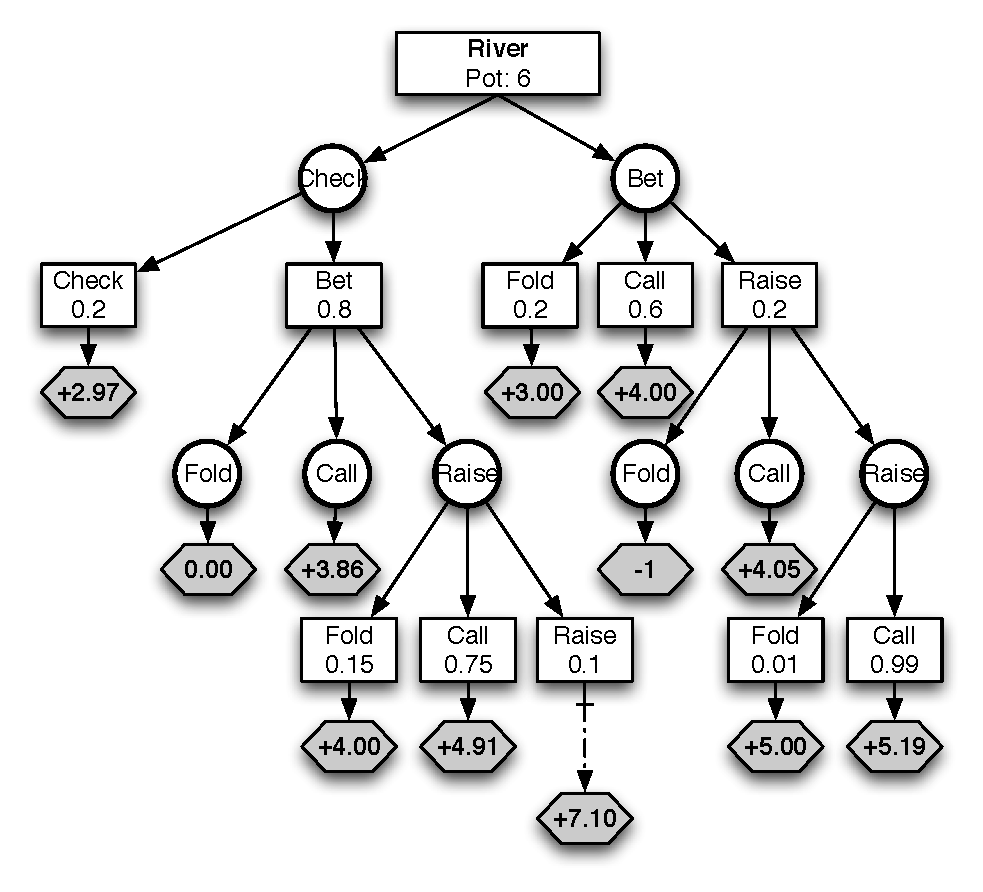
\includegraphics[width=\linewidth]{section03-gametree/figures/miximax}
\caption{A game tree with opponent modeling and hand evaluation for a river decision (example values taken from \cite{Davidson2002})}
\label{fig:miximax}
\end{figure}

Since the player is given a (very) strong hand, all leafs representing showdowns have a positive EV. In betting sequences where the opponent raises, the estimate is less optimistic, since the opponent is more likely to have a stronger hand. Backing up the values at the leaves, gives the estimates of the expected value shown in figure \ref{fig:miximax2}. We can compute, that the EV of checking is equal to 0.2 times the EV of the subtree where the player and the opponent checks, and 0.8 times the EV where the player checks and the opponent bets. In this given example, the player would proceed to Check, since the EV of checking is 4.59, higher than the 4.04 of betting.

\begin{figure}[!ht]
\centering
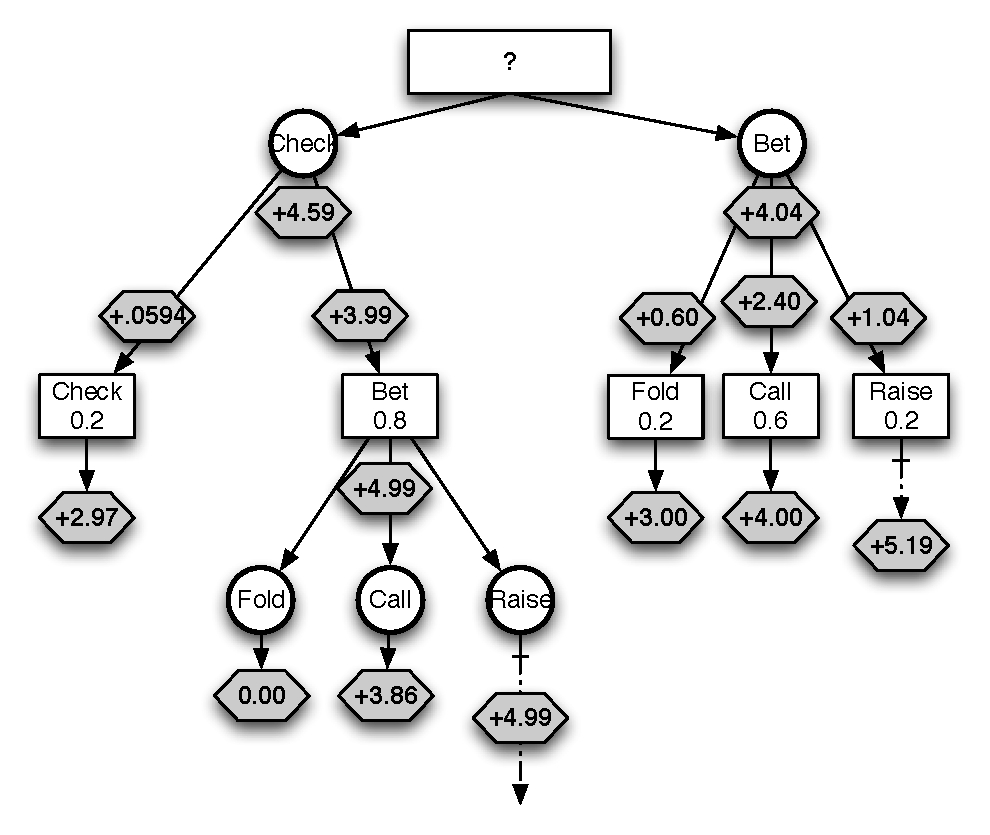
\includegraphics[width=\linewidth]{section03-gametree/figures/miximax2}
\caption{Example of the EV calculation for checking and betting for the decision in figure \ref{fig:miximax}}
\label{fig:miximax2}
\end{figure}

To repeat the calculations used in Miximax-Search (out of \cite{Davidson2002}, \cite{Schauenberg2006} and \cite{Billings2006b}): 

\begin{itemize}
	\item To calculate the expected value for one of the \textbf{players decisions}, the weighted sum of its children's values is used. The weights are the probability of the occurrence of a certain response from the opponent. Let $Pr(A_i)$ be the estimated probability that the opponent will respond with child move $i$ to the decision node $A$, and let $n$ be the number of legal options of the opponent. The EV of the player's action $A$ becomes:
\begin{equation}
	EV(A) = \sum_{i=1}^n Pr(A_i)\times EV(A_i)
\end{equation}
	\item To calculate the expected value for one of the \textbf{opponents decisions} we take the maximum EV of the children (the players responses). Here, the maximum is chosen for simplicity, to employ a mixed strategy, this can be modified to a more accurate function. Such strategies are mentioned in the next section \ref{sec:miximix}
	\begin{equation}
	EV(B)=max(EV(B_{fold}),EV(B_{call}),EV(B_{raise}))
	\end{equation}
Or in general, for n choices (like in no-limit poker)
		\begin{equation}
	EV(B)=max(EV(B_1),EV(B_2),...,EV(B_n))
	\end{equation}
	\item To caluclate the expected value of a \textbf{chance node} the subtree is expaned multiple times with each of the possible cards. For simplicity, like \cite{Billings2006b} we ignore the fact that certain cards might be less likely to be dealt, since they are more likely to be hold by the opponent in the foregone action sequence, and establish (like \cite{Davidson2002} that these outcomes occur uniformly at random. Let $(\ast)$ be a chance node for a board card and $n$ be the number of possible cards left in the deck (e.g. 44 on the river-card).
	\begin{equation}
	EV(\ast) = \frac{\sum_{i=1}^n EV(\ast_i)}{n}
	\end{equation}
	\item The expected value at a \textbf{leaf node} is the probability of winning the pot times the size of the pot, minus the cost of reaching the leaf node. If the leaf node is due to a fold then the probability of winning is 1.0 if the opponent foldet, and 0.0 if the player folded. If the leaf is a showdown, the probability of winning is estimated as best as possible. Possible estimations are discussed in chapter \ref{c:opponentmodelling} about opponent modelling. Let $L$ be a leaf node, $P_{win}$ the probability of winning the pot, $L_{\$pot}$ be the size of the pot, and $L_{\$cost}$ be the cost of reaching the leaf node.
	\begin{equation}
	EV(L) = P_{win} \times L_{\$pot} - L_{\$cost}
	\end{equation}
\end{itemize}
	

\section{Multiplayer games}

Although this thesis will focus on Heads-Up Poker with only two players, poker, like most games, isn't only played one-on-one, but more often against a larger number of players. The vast majority of poker players play most of the time on tables with 5 to 10 opponents (least at stakes lower than the so-called nose-bleed stakes with blinds like 500/1000\$ or higher).

Although most research in computer poker has been focused on heads-up play, I want to shortly summarize the challenges and possible adaptions for the algorithms presented so far.

\cite{Russell2003} explains the required adaptions to the basic game tree. To adapt, the expected values at each node in the game tree has to be replaced with a vector of expected values for each player taking part in the game.  For terminal states, this vector gives the utility of the state from each player's viewpoint. For two-player games a single value could be used because in zero-sum games, the payoffs are always mirrored.  To calculate these vectors, the utility function now has to return a vector (in poker, the new possibility of side-pots complicates this compared to the heads-up utility function).  Since for each new player a new set of decision nodes has to be added to the tree, the game tree grows much faster and deeper than in two player games. In Poker, this would probably require the implementation of difficult evaluation functions.

All this could still be managed computationally given enough resources. A much bigger problem is the accounting of the relations between the players. Multiplayer games often involve alliances - even though forbidden in poker, at least unconscious collusion is common. And if no such alliance building happens, it's still as good as impossible that each players plays exactly the same against each other player on the table.
For these reasons, multi-player games are inherently unstable, being subject to possible collusion between players. 

As \cite{Billings2006}�points out, two different move choices could be exactly equal in value for Player A, but could dictate whether Player B or Player C wins the game. Due to these very volatile conditions, a much better opponent modeling (for example, knowing each player's method of tie-breaking between equal moves) is necessary to obtain robust and reliable results.

\chapter{Opponent Modelling}
\label{c:opponentmodelling}

After having outlined the algorithms necessary to make a decision based on the game context, there still stays an unresolved issue; how to determine the probability distribution of an opponents possible action and the hands he might hold.  Both in computer as in human poker, a good judgement of the opponent is required. A player must be able to predict the opponents actions, as well as figuring out what cards he might hold. Essentially, the target is to estimate the missing information in this game of imperfect information. 

To achieve this, a model of the opponent has to be created. This model could be very generic; based on historic averages or game-theoretic optima, both very static models.  But playing good poker also includes adapting to a specific player, learning his strengths and weaknesses and exploiting them. To achieve this, the opponent model can't be merely static, but has to adapt to the current opponent, or even the current style the current opponent is playing. ideally, a good opponent model would never reaches a stable conclusion, but continue to adapt to the current opponent as well as his style at every moment.

Little surprising, as \cite{Pena1999} has shown, specific (based on observations of the the current opponent) opponent modeling outperforms generic opponent modeling.

To predict actions and cards, there exist a multitude of methods. From basically non-modeling but calculating the game theoretic best actions (used in all basic game theoretic methods of \cite{Gilpin2006} \cite{Johanson2007} or \cite{Miltersen2007}, used in \cite{Billings2006b} and \cite{Schauenberg2006} as a default prior of the model), to neural networks and decision trees.


\section{Optimal versus Maximal Play}
\label{sec:optimalvsmaximal}

One important consequence of imperfect information is that a complete strategy for a game like poker must include a certain degree of deception. It can by very rewarding to bluff (betting or raising with a weak hand) or slow play (playing a strong hand as though it were weak), not only because it might lead to winning a hand with weak cards, but also to add some noise to the revealed information. As \cite{Billings2006} explains, the requirement for such deceptions was one of the earliest results in game theory \cite{Neumann1944}. Essentially, it's always best to reveal as little information as possible, to act as unpredictably as possible.

In Poker, the target of deception tactics is it to disguise the strength of a hand (information hiding), and to create uncertainty for the opponent. As \cite{Billings2006} explaines, the relative balance of these deceptive plays (and of responses to the opponent's actions) is of critical importance. Any inappropriate imbalances necessarily imply the existence of statistical biases, patterns, or other weaknesses that are vulnerable to exploitation. Since there may be many ways of obtaining the desired balance of plays in poker, the players have some discretion in how they actually achieve that balance. In essence, it might not matter if, in a specific situation, a player bluffs or doesn't, as long as a certain bluff frequency in this and similar situation is maintained. As a often stressed result, there is in general no single best move in a given poker situation  \cite{Sklansky1999} \cite{Chen2006} (but in theory, there might be a best distribution of moves). This is a huge difference to perfect information games, where a single move can be determined to lead to the game-theoretic maximum.

As \cite{Billings2006} notes, correct play in an imperfect information game requires probabilistic mixed strategies, where different moves are chosen some fraction of the time in identical circumstances. In a perfect information game though, a deterministic pure strategy (always playing one particular move in a given situation) is sufficient to obtain
the game-theoretic value although the player may choose randomly from a set of equally valued moves).

It's important to understand the difference between optimal and maximal play. Optimal play is a result of a equilibrium strategy. In games like poker, where weaknesses of an opponent be systematically exploited, an equilibrium strategy is only maximal against an equilibrium playing opponent (an opponent without any exploitability).

In a Nash equilibrium strategy, no player has an incentive to deviate from the strategy, because the alternatives only lead to equal or worse results. This simply maximizes the minimum outcome. In essence, this is a defensive strategy which assumes the opponent plays perfect, and the player only tries to not loose. In practice, outside of very simple games like tic-tac-toe, no such player exists, especially not in poker. Only a very small fraction of games have been game theoretically solved. And it's questionable if some of them ever will, since the search space for games like chess, go or larger poker games is just too enormous.

Not only might a Nash equilibrium player not play an optimal strategy, in certain situations he might not even defeat a non-optimal opponent.  For example, in the game of rock-paper-scissors, the equilibrium strategy is to select an action uniformly at random among the three choices. Using that strategy means that no one can defeat you in the long term, but it also means that you will not win, since the equilibrium player has an expected value of zero against any other strategy.

Unlike rock-paper-scissors, poker is a game in which some strategies are dominated, and could potentially lose to an equilibrium player. Nevertheless, even a relatively weak and simplistic strategy might break even against a Nash equilibrium opponent, or not lose by very much over the long term. 

In contrast, a maximal player can make deviate from an "optimal" strategy when it believes that such a move has a higher expected value.  \cite{Johanson2007} employs such a strategy in his approach for a best response strategy, based on different $\epsilon$-equilibria strategies.

Considering the case of rock-paper-scissors where a opponent has played "rock" 100 times in a row, a Nash equilibrium program is completely oblivious to the other player's tendencies, and does not attempt to punish predictable play in any way. A maximal player, on the other hand, will attempt to exploit perceived patterns or biases. This always incurs some risk (the opponent might have been setting a trap with the intention of deviating on the 101st game). A maximal player would normally accept this small risk, playing "paper" with a belief of positive expectation \cite{Billings2006}. Similarly, a poker program can profitably deviate from an equilibrium strategy by observing the opponent's play and biasing its decision-making process to exploit the perceived weaknesses.

If a poker algorithm were based on a true Nash equilibrium solution, then no human or computer player could expect to defeat it at all in the long run. However, all current poker programs are only an approximation of an equilibrium strategy (\cite{Johanson2007}, \cite{Gilpin2007} etc.), and it will not be feasible to compute a true Nash equilibrium solution for Texas Hold'em in the foreseeable future. There is also an important practical limitation to this approach.

Additionally, simple equilibrium approximations are unintentionally exploitable. Since they apply a fixed strategy, a strong human player can systematically explore various options, probing for weaknesses without fear of being punished for using a highly predictable style. Moreover, the key to defeating all human poker players is to exploit their highly
non-optimal play. 
When humans play games, especially at a more professional level, they analyze previous games played by their opponent to become familiar with the strategies used by the opponent, its strengths and weaknesses. Even when playing against
an unknown player, they will create, during the game, a model of the opponent, based on some features of the opponents behavior. To compete at such a level of skill, a computer poker program would also be required to be able to adapt to an opponents play and adapt to dynamically changing conditions. \cite{Billings2006}

\section{Challenges in Opponent Modelling}

As we have seen in the last chapter, for poker, we need our opponent model to predict two things in the game tree. First, what action a player might take, given a certain situation. Second, how strong his cards might be, given a certain situation. As we will see, this task faces challenges, shared with many other machine learning or data mining problems. \cite[p.36-37]{Davidson2002} summarizes them as follows:

\begin{itemize}
	\item \textbf{Uncertainty:} Thanks to the numerous unknown cards in a game, poker games always include a great deal of noise. Each hand of poker can be completely different to the previous one, simply because of the variance of cards dealt. Both to the hands as well as to the board. Because of this, a very large number of hands must be played bevor even very common situations are encountered several times.
	\item \textbf{Missing Information:} Only the player and his opponent play to the end of a hand, cards are actually shown. In heads-up only a very small percentage of hands are revealed. Because of this, the opponent model can only be verified on the very few hands the player as well as the opponent take to the showdown. Additionally, these hands are obviously heavily biased (players always try to avoid taking bad hands to a showdown - either by folding or by getting the opponent to fold).
	\item \textbf{Unknown Dimensions:} It's never completely known what variables, and how many of them affect how a player plays a hand. Some factors might be much more important than others, and some are not of concern for every player. One might put importance into their position in the betting round, while others only adapt lightly to their position. To find the appropriate correlations is important, but very difficult. 
	\item \textbf{Intuition:} Thanks to intuition and past experience, good human Players are able to form an elaborate model of the opponent based on only a small number of observations. If experienced, they can also challenge their model to test a theory about an opponent. In contract, most machine learning methods typically need a large number of observations. These methods are not only slow, but also passive.
	\item \textbf{Multiple Levels:} If we model an opponent based on how he plays against another player, we can't regress his behavior playing against us, at least not if he is also modeling his opponents. So we need find a "pure" model (the opponents behavior minus his adaptations to a certain player) as well as how he models opponents. (or how he models how we model, etc...)
	\item \textbf{Moving Targets:} To play good poker also means to constantly change once behaviour, simply to add noise to the opponents observations. This and the fact that the opponent might change his model about us, presents the problem that the opponent model has to be changed constantly, and that once we achieve a solid model, this model is already outdated.
\end{itemize}

To summarize, opponent modeling contains the typical characteristics of most machine learning problems;noise, uncertainty, unknown relations, and the need to quickly generalize from a small set of examples - often with wrong or misleading data.  


\section{Opponent Modelling Techniques}
\label{opponent-modelling-techniques}
As we don't know the hands of the opponent, we can't perfectly predict what an opponent play, but a distribution of actions. Considering machine learning, an opponent model is a predictor of the opponent. In the data mining approach outlined later, it's simply a matter of classifying a certain decision point or game situation into possible opponent action classes. \cite[p.37]{Davidson2002} outlines the basic methods of opponent modeling, which are shortly outlined hereby. Most of these techniques can also be used in the later introduced \textit{Weka Data Mining Framework} and can be applied to the algorithm described in chapter ~\ref{c:imperfectinformation}.

\subsection{Expert Systems}
Expert Systems are implementing a generic opponent model, crafted after human knowhow and implemented as a set of rules. One way would be to predict an opponent action based on our own betting strategy, or advice out of a poker strategy book. Expert Systems normally aren't very effective, since they scale very bad for complex problems, but they are a good start for a opponent model, per example before any knowhow about a specific opponent could be collected.

\subsection{Statistics}
\label{s:statistics}
Another rather obvious method of predicting an opponent is observing his past actions, assuming he would act the same or similar in the future. If he raised 10\% of our bets on the flop, after a lot of action already happened pre-flop, one might infer that the next time such a situation occurs, the possibility of our opponent to raise is 10\%.


\cite{Davidson2002}'s opponent modeling effort was based on a collection of simple statistic information. For example, a basic system distinguished only twelve different contexts a player might encounter. These twelve contexts differ only in the betting round (pre-flop, flop, turn, or river), and the betting level (zero, one, or two or more bets)

The resulting history table is essentially a set of conditional action probabilities such as \linebreak $P(OneBetToCall,stage=river)$ - describing the probability of a raise, given there was one bet this hand so far, and the decision will be made on the river. 

However, this is a very limited definition of distinct contexts, since it does not account for many relevant properties, such as the number of active opponents, the relative betting position, or the texture of the board cards (eg. whether or not many draws are possible). 

Establishing a suitable set of conditions for defining the various situations is not an easy task. There are
important trade-offs that determine how quickly the algorithm can learn and apply
its empirically discovered knowledge. If a context is defined too broadly, it will fail to
capture relevant information from very different circumstances. If it is too narrow,
it will take too long to experience enough examples for each scenario, and spotting
general trends becomes increasingly difficult. Equally important to deciding how
many equivalence classes to use is knowing what kinds of contextual information
are most relevant in practice.


One such model, is the histogram-based approach by \cite{Schauenberg2006} and \cite{Billings2006b}.  Essential for using such statistical modeling, it a good abstraction of the game context. 

In poker, two situations rarely happen twice, even after millions of hands, so the need for generalization arises. For their Miximax-based agents,  \cite{Schauenberg2006}  and \cite{Billings2006b} used a collection of histograms with different levels of generalization. To learn faster and base their inferences on more observations, \cite{Billings2006b} use various different context trees with different granulation, and combine multiple contexts with high mutual correlation.  This allows them to generalize the observations made, and apply that knowledge to other related situations.

The context tree they used is an explicit representation of the imperfect information game tree, having the same skeletal structure with respect to decision nodes. Chance nodes in the tree are represented implicitly (all possible chance outcomes are accounted for during the EV calculation).

A leaf node of the context tree corresponds to all of the leaves of the game tree with the same betting sequence (regardless of the preceding chance nodes).

Associated with this is an efficient data structure for maintaining the empirically observed action frequencies and showdown histograms for the opponent. For this they use a trie, based on the natural prefix structure of related betting sequences.
 
The finest level in the abstraction is the context tree itself, where every possible betting sequence is distinct, and a different histogram is used for each. This basically is a reproduction of all possible game situations.  The
opponent action frequencies are determined from the number of times each action was chosen at each decision node (they also used a decay factor, to strengthen recent observations). Unfortunately, having little data in each class will result in unreliable inferences.

With testing, they concluded, that the most coarse-grained abstraction would solely hold the sum of the total number of raises by both player (no longer distinguishing which player initiated the action) - in total only nine distinct classes. Despite the crudeness of this abstraction, the favorable effects of grouping the data is often more important than the lower expected correlations between those lines of play. Another similar type of coarse-grained abstraction considers only the final size of the pot, adjusting the resolution (i.e. the range of pot sizes) to provide whatever number of abstraction classes is desired.

A less coarse-grained abstraction groups all betting sequences where the opponent made an equal number of bets and raises throughout the hand, ignoring what stage of the hand they were made. A finer-grained version of the same idea maintains an ordered pair for the number of bets and raises by each player.

 One problem with a statistical approach to opponent modeling is the zero frequency problem, when there has not yet been any observations for a given context - and more generally, how to initialize the context tree with good default data. \cite{Billings2006b} depend on results from Nash equilibrium strategies, to devise default data based on the assumption of optimal play.

\cite{Schauenberg2006} and \cite{Billings2006b} use various different abstractions of situations and weights them differently before predicting a situation. One extreme would be the exactly same situation, another every other situation with the same amount of player actions in the hand so far. Based on this  \cite{Billings2006b}  specified 8 different abstractions which he averaged to calculate the action distribution of possible actions. \cite{Schauenberg2006}, \cite{Billings2006b} and \cite{Davidson2002} don't take the public board cards into consideration when looking for similar situations.

Establishing a suitable model on how broad or narrow a situation should be specified is no easy task. There's an obvious trade-off of being either to narrow, so there are not enough samples to base assumptions from, or being to broad, so estimations will be vulnerable to over-fitting. 

Furthermore, each player acts differently. One might be very affine to flush draws and play them very aggressively, another might put a lot of weight in his current chip stack before deciding how to act. To model this, a meta-model would have to be built of the player, to specify which parameters are weighted how much in the modeling process. 
Using data mining algorithms and a very large set of parameters might be a good approach for this problem, since figuring out the weight of the different parameters is a common problem in other classifying problem.

As the abstraction system of  \cite{Billings2006b} is hierarchical, there also has to be spent some consideration into the weight of the different tiers of abstraction. This is based on the number of actual observations covered at each level, striving for an effective balance, which will vary depending on the opponent.

Their method of combining different abstraction classes is based on an exponential mixing parameter (e.g. $m = 0.95$). With the lowest-level context tree (no abstraction) be called $A_0$, a fine-grained abstraction be called $A_1$, a cruder collection of those classes be called $A_2$, and the broadest classification (only pot-size or only count of bets) level be called $A_3$. 

Suppose the showdown situation in question has five data points (earlier observations) that match the context exactly, in $A_0$. This data is given a weight of $1-m^5 = 0.23$ of the total. If the next level of abstraction, $A_1$, has 20 data points (including those from $A_0$), it is assigned $1-m^20 = 0.64$ of the
remaining weight, or about $50\%$ of the total. The next abstraction level might
cover 75 data points, and be given $1-m^75 = 0.98$ of the remainder, or
$26\%$ of the total. The small remaining weight is given to the crudest level of
abstraction. Thus all levels contribute to the overall profile, depending on how
relevant each is to the current situation.

After each hand is finished, the observations made must be applied to the histograms in the context tree.  The action decisions made by the opponent are used to update the betting frequencies corresponding to the sequence of actions during the hand, while the shown cards (respectively, the hank rank of the cards) are used to update a leaf node histogram.

The context basically represents the imperfect information tree which is searched when looking for the correct action. It has the same decision nodes, but is lacking the explicit representation of the chance nodes. A leaf node of the context tree corresponds to all of the leaves of the game tree with the same betting sequence (regardless of the preceding chance nodes).

Since in poker a situation rarely occurs twice, many thousands of games may have to be observed before a reliable histogram of an opponents actions might be constructed. Worse, by the time enough observations have been made, the collected information might already by outdated.

As it's common for human players to often and quickly change their style of play, knowledge has to be accumulated very quickly, and possibly have a preference toward more recent observations. In the best case, the opponent model should adjust beginning with the first action of an opponent. 

As \cite{Billings2006b} highlights, this might be a more challenging learning task than most of the problems studied in the machine learning and artificial intelligence literature. Unlike
most Markov decision process (MDP) problems, the model isn't trying to learn a static property of a domain (we assume that the default model already fits a generally good poker player)  but rather the dynamic characteristics moving target.

In order to give a preference toward more recent data,  \cite{Billings2006b} use a factor to gradually "forget" old observations using an exponential history decay functions. Each time an observation is made in a given context, the previously accumulated data is diminished
by a history decay factor, and the new data is only added after this decay.

\subsection{Neural Networks}
\label{s:neural-networks}
Neural Networks can be used for a variety of classification tasks. The simple \textit{perceptron learning rule} can be used to learn the weights for a linear hyperplane - similar to regression models. 

Neural Networks are easy to build automatically without any domain-specific knowledge and tend to provide reasonable accuracy, especially in noisy domains. This ability suits well in problems with stochastic elements - such as poker or backgammon. As \cite{Davidson2002} mentions, Neural Networks have been used with success in backgammon programs (such as the already mentioned TD-Gammon by \cite{Tesauro2002}).


A neural network consists of neurons, or nodes, which are connected to each other
by weighted directed edges. Problem data is fed into input nodes, which are connected to internal (or "hidden") nodes, which themselves are connected to a set of output nodes (the solution data).

 The weighted connections between these nodes can be both of negative or positive weight. They transform the signal from the input nodes, through the the internal nodes to the output nodes. Similar to biological neurons, the internal nodes "fire", if the weighted sum of all connections entering reaches a certain threshold. If this threshold is reached, they send a signal to the connected nodes further down the network - either output nodes or another layer of internal nodes. The output of a node can be either discrete (they send a 1 if the threshold is reached, and a 0 if it isn't) or continuous if a sigmoid function is used to produce a smoother output. 

\begin{figure}[!ht]
\centering
\includegraphics[width=0.55\linewidth]{section04-opponentmodel/figures/simple-neural-network}
\caption{Simple neural network example (from \cite{Davidson2002})}
\label{fig:simple-neural-network}
\end{figure}

Figure \ref{fig:simple-neural-network} shows a basic neural network, with the four input nodes on the top, two internal nodes (one hidden layer) in the middle, and the single output node on the bottom. Weights are represented by the thickness of the connection.

In this example, the internal neurons use a discrete threshold function to decide their outputs, but the output neuron uses a sigmoid function to decide its output. The two input neurons have different thresholds for firing. This is known as a bias, and each neuron can have a positive or negative bias affecting its behaviour.


\subsubsection{Backpropagation}
To "learn" these weights, a algorithm called back-propagation is used. With back-propagation, the correct answer of a training instance is worked backwards through the neural network, starting from the output and ending back at the input. The output on node $i$, $O_i$ is compared to the correct answer (the correct classification) to calculate the network's error $E_i$. Starting with the weights at the output nodes, the weights are adjusted until the error $E_i$ is minimized. Each weight is adjusted proportionally to its contribution to the error.

To calculate the contribution to the error for a connection $W_j,i$ from a internal node $j$ to an output node $i$, the error at the output node $E_i$ is multiplied by the derivative of the activation g along the input value $I_i$ to the node.

	\begin{equation}
	\Delta_i = E_i \ast g' I_i
	\end{equation}

This equation determines both the direction of the error, as well as the influence of a specific weight to the error. The weight is updated by adding $\Delta_i$ times the activation level ($O_j$ ). To adjust the amount of chance, a learning rate is applied to increase or decrease the amount of change made to the weight for each training example. The higher the learning rate, the faster the network adjusts, but the longer it takes to reach a stable condition.

	\begin{equation}
	W_{j,i} \Leftarrow W_{j,i} + \alpha  \ast O_j  \ast \Delta_i
	\end{equation}

After updating the weights at the output layer, the error is propagated further up the network. To calculate the error at an internal node connection, the following equation is applied.


	\begin{equation}
	\Delta_j = g' I_j \sum_i W_{j,i} \Delta_i
	\end{equation}

With each additional training example, the error in the network is determined and the
weights are modified using this  method. After several training iterations, the network starts to converge to a set of weights that minimize the error over all examples in the
training set. To additionally stabilize the back-propagation progress, most algorithms additionally try to minimize the error over multiple samples by reseting the network to a earlier state, should the new weights result in a weaker accuracy.

Further refinements for back-propagation algorithms are explained in in \cite{Russell2003}, \cite{Witten2005} and \cite{Rumelhart1986}. 

\subsubsection{Poker Neural Nets}
\cite{Davidson2002} trained a standard multi-layer perceptron (also known as feed-forward neural net) on contextual data collected from online games against human opponents. His network contain a set of eighteen inputs corresponding to properties of the game context, such as number of active player (his program - \texttt{Poki} - was built for ring games), texture of the board, opponent's position, the full list is shown in table \ref{fig:poki-input-nodes}.

\begin{table}[!ht]
  \begin{tabular}{ l|c | l}
\textbf{\#} & \textbf{Type}�& \textbf{Description}�\\
 \hline
 0  & real & immediate pot odds\\
 1 & real & bet ratio: \textit{bets/(bets+calls)} \\
 2 & boolean & committed (has put money in the put this round) \\
 3 & boolean & one bet to call \\
 4 & boolean & two or more bets to call \\
 5 & boolean & betting round = turn \\
 6 & boolean & betting round = river \\
 7 & boolean & last bets called by player > 0  \\
 8 & boolean & player's last action was a bet or raise \\
 9 & real & 0.1*numPlayers \\
 10 &boolean & active players is 2 (heads-up) \\
 11 & boolean & player is first to act \\
 12 & boolean & player is last to act \\
 13 & real & estimated Hand Strength for opponent \\
 14 & real & estimated Hand Potential for opponent \\
 15 & boolean & expert predictor says they would call \\
 16 & boolean & expert predictor says they would raise \\
 17 & boolean & Poki is in the hand \\

 \end{tabular}
 
\caption{Poki neural network input nodes \cite{Davidson2002}}

\label{fig:poki-input-nodes}
\end{table}

The output layer consists of the possible actions an opponent might take (this version of \texttt{Poki} was built for limit-poker, so theres only three possible actions: fold, call or raise). By graphically displaying the relative connection strengths, it's possible to determine which input parameters have the largest effects on the output. After observing networks trained on many different opponents, it is clear that certain factors are dominant in predicting the actions of most opponents, while other variables are almost completely irrelevant (\cite{Davidson2002}).

The inputs encode the knowledge of the player about the game context. All inputs are encoded to values between zero and one. The current betting round for example is encoded using two boolean input. On the flop, both inputs \#5 and \#6 are zero, if it is the turn, \#5 is set to one, and so on. \cite{Davidson2002} has also included additional expert information about the current context. Input \#13 and \#14 are the estimated hand strength - something which isn't necessairy to know with the miximax-algorithm explained in chapter \ref{c:imperfectinformation}. Inputs \#15 and \#16 indicate what an expert-buildet formula based system would do in this context. 

Figure \ref{fig:poki-neural-network} shows a resulting neural network from \cite{Davidson2002} after a few hundred hands trained from plays by a particular opponent. 


\begin{figure}[!ht]
\centering
\includegraphics[width=0.7\linewidth]{section04-opponentmodel/figures/poki-neural-network}
\caption{The resulting neural network for Poki \cite{Davidson2002}}

\label{fig:poki-neural-network}
\end{figure}

The inputs are on the top, with the activation level painted as black dots, ranging from zero to one and the thickness of the lines representing the weights (black being positive, grey being negative). In this example, as \cite{Davidson2002}  explains, the connections from the input for representing a raise as the last action can be seen as very heavy, indicating a high correlation between a raise and what the opponent will do next. The outputs show that the network is predicting that the opponent will most likely bet again, with a small probability of checking. This makes intuitive sense - if a player has just bet, there is a very small chance they will fold, and a much larger chance that they will call or raise. 
Examining the graphical representations of neural networks reveal the features that have the highest correlations with the opponents actions. \cite{Davidson2002} mentions that very strong correlations could differ significantly between specific opponents. Some might be more tempted to continuation bets, putting significance on a stringent betting line, while other players actions correlate more with the texture of the public board.

Later on, \cite{Davidson2002}  used these insights to add the player's last
action to the context of the action frequency statistics. This reportedly improved
the accuracy of the statistics by an additonal 10-to-20\%.

Overall, \cite{Davidson2002} came to the conclusion, that the biggest drawback with neural networks is that they aren't trained on a proper probability distribution, but the actual event. For this reason, they don't output a distribution which is skewed to the most possible outcome and not the most accurate distribution. Nevertheless, they allow a much deeper evaluation, since the underlying logic can be graphically illustrated and analyzed. Wrong learning tendencies can be recognized and avoided this way. 


\subsection{Decision Trees}
Decision trees are another well known way to solve classification problems. Nodes in a decision tree involve testing a particular attribute. In general, the test at a node compares an attribute value with a constant. Leaf nodes give a classification that applies to all instances that reach the leaf, or more suitable for poker, a probability distribution over all possible classifications. A unknown instance is routed down the tree according to the values of the attributes tested in successive nodes, and when a leaf node is reached, the sample (or instance in the data mining framework explained later on) classified according to the class assigned to that specific leaf. 

\begin{figure}[!ht]
\centering
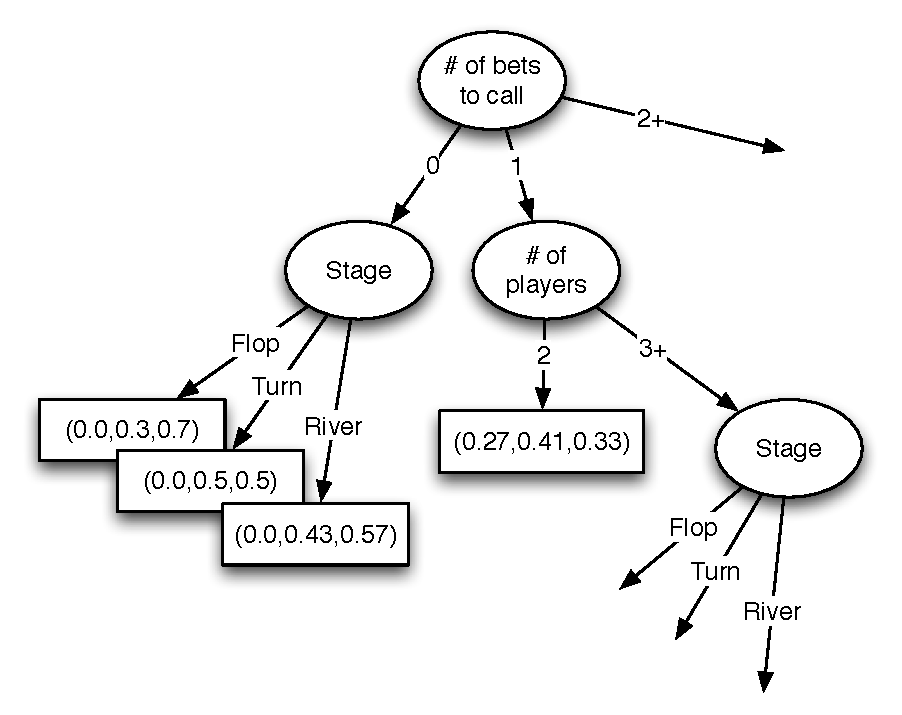
\includegraphics[width=\linewidth]{section04-opponentmodel/figures/decision-tree}
\caption{A possible decision tree example (used in \cite{Davidson2002})}
\label{fig:decision-tree}
\end{figure}

\cite{Davidson2002} used a Decision Tree Induction software \cite{Utgoff1989} to study decision trees for action prediction. Due to the high amount of noise in poker, they opted to train with tree pruning. Unfortunately, even trees with pruning activated were not as noise-tolerant as neural networks. Still, they have shown several benefits. They can output accurate probability distributions over the available choices, something neural networks can't do (as seen in the last chapter, neural networks are much better predicting the correct action than producing an accurate distribution).
Decision trees share the benefit of human readability with neural networks. They easily be represented in a very human-understandable format, although in poker this might only be of use in the debugging stage and isn't of much use once the abstraction of the contexts and the learning parameters have been fixed.

\cite{Davidson2002} concludes, that decision trees are not as accurate as neural networks, but are still a interesting avenue for further exploration.

\subsection{Alternative opponent models}

 \cite{Ponsen2008} explored an interesting bayes-relational opponent modeling system that predicts both actions and outcomes for human players in the game of No-Limit Texas Hold�em poker. His approach uses two models.  One model - the prior - is trained offline, based either on past games or some optimal values derived from equilibria calculations. 

Then, during a game, instead of updating this prior during the game, his systems learns a second model during the game, which specifies a distance function to the prior.

An action in \cite{Ponsen2008}�is viewed as an example consisting of tuple $(i,p,a_i,r_p,H_{i-1},B_i)$ of the action $a_i$ performed at stage $i$ by a player $p$, together with the outcome $r_p$ (outcomes can either be a fold before the end of the hand, a win without showing hands or showing a certain pair of cards), the the board $B_i$ and the betting history $H_{i-1}$.

He then considers the mixture $D_{p+\ast}$ of two distributions: the distribution $D_\ast$ of randomly drawn tuples from all players (the data available to the prior) and the distribution $D_p$ of randomly drawn examples from a specific opponent (say the observations in the game so far).

A theoretic learning problem then is to predict whether a randomly drawn tuple $x$ originated from $D_\ast$ (the general observations) or from $D_p$ (the distribution of the current opponent).  For a given learning setting (either predicting actions from outcomes or predicting outcomes from actions), according to \cite{Ponsen2008}�it then is easy to generate examples from $D_\ast$ and $D_p$, labeling them with $\ast$ or $p$ and learning the function $P(D_p|x)$, giving for each example the probability the observation originates from the distribution of the current opponent. 

With such a learned differentiating model, \cite{Ponsen2008}�is able (after some transformations) to formulate the final predictor 
\begin{equation}
	 P(x|D_p) = \frac{P(x|D_*) \cdot P(D_p|x)}{1-P(D_p|x)}
\end{equation}

$P(x|D_{\ast})$ being the learning prior and $P(D_p|x)$ the differentiating function. To predict a distribution of actions, one would simply create the possible tuples at the current game context and calculate the probability for each of them being part of the players set of action tuples.

To calculate the prior $P(x|D_{\ast})$ \cite{Ponsen2008}�also applies this approach to learning a differentiating function between a uniform function and the distribution formed by all examples from all players in a generic dataset.

Unfortunately, common data mining frameworks like \textit{Weka} do not support such algorithms, and the relational probability learning used by \cite{Ponsen2008}�isn't freely available. Reportetly, this approach showed impressive learning speed which already started to improve prediction rates after as little as 200 games, which is much faster than other methods, like the ones used in \cite{Billings2006b} and \cite{Schauenberg2006} which required thousands of hands to improve.

\section{Choosing the parameters and attributes}
Before learning a classification scheme with a machine learning algorithm, the data has to be preprocessed and abstract. 
As mentioned before, no-limit poker holds virtually unlimited combinations of game factor - the same context rarely occurs twice. Two ways to represent abstracted game contexts have been shown. \cite{Billings2006b} and \cite{Schauenberg2006} use multiple context trees - or trie - to store various abstractions of the current game context. Their two extrema are the not-abstracted game context with the exact action sequence leading to the current situation, and the game context simply represented by the number of actions that have happened so far.

For more conventional classifiers as used in the \textit{Weka}�Data Mining Framework, the game context have to be represented as a dataset (specifically a relation) of tuples called instances. 
Fortunately, to build the structure of such instances, much of what had been proposed by \cite{Davidson2000} and \cite{Davidson2002} as attributes of a game context in a neural network (see  \ref{fig:poki-input-nodes}) can be reused as a basis for my own abstraction of a game context.Nevertheless, the basic abstractions can be used for our own abstraction of a game context.

The model from \cite{Davidson2002} was built be used in ring poker, includes some expert knowledge (like a prediction from an additional expert system) and is used in a different game solving algorithm, so not all attributes are usable for our model. 

After experimentation, the following attributes have shown to be a solid approximation of a game context in Heads-Up No-Limit Texas Hold'em.

\begin{itemize}
\item Obviously, the observed (or to be predicted) \textbf{Action} �or \textbf{Hand Strength} �has to be part of each instance.
\item �\textbf{Bet counts}  for both players are added as an attribute, providing a measurement of aggression so far.
\item Since, unlike in Limit Poker, the \textbf{pot size} does not necessarily correlate with the number of bets and calls, it has to be added. In Models for limit poker, this wasn't necessary, as the number of bets is already an attribute. 
\item As mentioned in the section about neural networks, there is a strong correlation between the  \textbf{previous actions} and what is done next, so they have to be part of an abstracted game context. I opted to add both the action of the acting player, as well as the now observing player which did the last action. This allows the model to learn the basic poker rules (checking isn't allowed after a bet, folding after a check is a bad move in any case).
\item To take the importance of position into consideration, there is also a boolean attribute for the fact if the acting player is currently playing on the \textbf{button position}. 
\item Obviously, the \textbf{stage of the game}� has a great influence on the actions a opponent might conduct. Since cards are always shown at the river, this attribute is redundant when predicting the hand strength of a player.
\end{itemize}�
 \cite{Billings2006b}�achieved strong playing performance without taking the board into consideration. Nevertheless, I still regarded the lack of such information a great disadvantage and added three attributes which account for the structure of the public board: 

\begin{itemize}
\item The \textbf{number of face cards} �dealt for a general assessment of the strength of the board. I initially used the hand strength (how strong a hand would be if it only played with the public cards) for this, but datasets with a count of face cards have shown better prediciton accuracy for an opponents hand strength (without any influence on the action prediction) in initial experiments.
\item The \textbf{number of cards with the same suit} �and the \textbf{number of connectors}�(hands usable to build a straight)  assess the possibility of a draw for a straight or a flush.
\end{itemize}�

\chapter{Building the opponent model}
After exploring the fundamental principles and techniques for opponent modeling and specifying a set of attributes for an abstraction of a game context, this chapter now focuses on the implementation of such opponent models.

As a basic starting point, the \textit{Weka Datamining Framework} (\cite{Hall2009}) was used. \textit{Weka} is a collection of machine learning algorithms for a variety data mining tasks. The algorithms can either be used in the accompanied application, or reused directly in a java program. \textit{Weka} also contains the necessary interfaces and data types to develop new or custom machine learning schemes.

It already includes a variety of Decision Tree and Neural Network Algorithms, which allow experimentation with the techniques outlined in the previous chapter.  And can be reused in Java programs like the final implementation of a poker agent in  chapter \ref{chap:implementation}.

\section{Aquiring a Training Dataset}
Before focusing on the algorithms, a training dataset has to be acquired. I have chosen to use the large (and free) dataset of the past matches in the \textit{The Annual Computer Poker Competition}. \textit{The Annual Computer Poker Competition} is a recurring competition of the current state of the art achievements in computer poker. Each year held during a artificial intelligence conference, it's objective is to "\textit{is to benefit artificial intelligence by promoting, aiding, and evaluating research in computer poker}." Besides providing interesting results, this competition also produces a huge log of hundreds of thousands hands played. I used these logs (\cite{Hawkin2009}) to extract all game context  observed by different players during the game and their responses to them. Unlike hand histories from other sources like online poker sites, this data is free and provides hundreds of thousands of hands per opponent, instead of probably only a few hundreds per opponent. Thanks to the small number of competitions and the fact that they all matched each other in a round robin tournament, the strength of play can also be estimated. 
 
    \begin{lstlisting}[captionpos=b, caption=Example Gamestate History, label=logFile, breaklines=true]

## GAMESTATE Version 2.0
## type: DOYLE NOSTACKBOUND
# Outcomes of hand are shown in the form:
# <PLAYERS>:<HANDNUMBER>:<BETTING>:<CARDS>:<NETONHAND>
# Players are listed in seat order:big blind (or button or dealer) is listed first.
# Cards on the preflop are in seat order, divided by vertical lines |.
# The net on won or lost on a hand (in small blinds) is last, and is in seat order.
HyperboreanNL-BR|BluffBot4:0:b1b2r7c7/r81f:Kh2d|5dJs/9h4c3s:7|-7
BluffBot4|HyperboreanNL-BR:1:b1b2c2c2/c2r41f:7s5h|3sAh/9d8d4h:-2|2
HyperboreanNL-BR|BluffBot4:2:b1b2r5c5/r67f:8h9c|TsQh/8d7d2s:5|-5
BluffBot4|HyperboreanNL-BR:3:b1b2c2r8c8/r22c22/c22c22/c22r36f:3d4d|QdJd/5h7cQc/4s/Qs:-22|22
HyperboreanNL-BR|BluffBot4:4:b1b2r7c7/r81f:7sKd|3c3h/Ah2h9s:7|-7
  \end{lstlisting}
 
To make these histories usable for training in \textit{Weka}, they first have to be preprocessed into the game contexts expected by the learning algorithms. Listing \ref{logFile} shows an excerpt of the first few lines of such a raw game-state history - it follows the syntax explained in \cite{Zinkevich2007}. Listing \ref{arffFile} shows the same match after preprocessing from the perspective of \textit{HyperboreanNL-BR} observing \textit{BluffBot4}. All Pre-Flop actions have been removed, since the implementation is only used on Post-Flop decisions, and the continuos chain of actions has been converted in abstracted game contexts.

  \begin{lstlisting}[captionpos=b, caption=Example ARFF Export, label=arffFile]
@relation HandActions

@attribute PlayerAction {f,k,c,b1,b2,b3}
@attribute PotSize numeric
@attribute BetCountActingPlayer numeric
@attribute BetCountObservingPlayer numeric
@attribute LastActionActingPlayer {f,k,c1,c2,b1,b2,b3}
@attribute LastActionObservingPlayer {f,k,c1,c2,b1,b2,b3}
@attribute ActingPlayerOnButton {true,false}
@attribute FaceCards numeric
@attribute DeckSuited numeric
@attribute DeckConnectors numeric
@attribute GameStage {pf,fp,tn,rv}
@attribute TotalActionCount numeric

@data
f,88,1,1,b2,b2,true,0,1,2,fp,2
k,4,0,0,k,k,false,0,2,2,fp,0
f,43,0,1,k,b2,false,0,2,2,fp,1
f,72,1,1,b2,b2,true,0,2,2,fp,2
b2,16,2,0,b2,c2,false,1,2,0,fp,2
  \end{lstlisting}
  
For each contestant, a few million actions and hundreds of thousands of hands were extracted from the hand histories of the competition in 2009. These could then be used to both build opponent models or benchmark them.
 
\section{Updateable Data Mining Algorithms}

Building a generic opponent model from historic data is only the starting point for a good model of a poker player. After this, the model needs to be updated to the specific opponent currently playing against a player. Learning a generic opponent model a player teaches the groundwork to deduce effective poker strategies by searching the game tree. But as stated before, playing the right move only guarantees not loosing the game. To win, the player has to exploit specific style of the current opponent. This requires the opponent model to be adjusted during the game, not only to the current opponent, but also to the style he currently employs, as is common for top human players to radically change their style of play many times over the course of a match. 

This must be an ongoing process, since we may need to keep up with a rapidly changing opponent. All in all, there are a two important of requirements such a data mining algorithm needs to fulfill to be usable in the context of a poker program: 

\begin{enumerate}
	\item I must be updateable online, after having trained as a default model with batch processing. The faster it adapts the better, but it still should stay robust over the course of a game.
	\item Classification must be as fast as possible. As each decision requires a game tree of hundreds of thousands of decision nodes and showdown nodes, classification at each such node can only take a fraction of a millisecond.
	\item Nominal Classification must be supported. Both action as well as hand classification require an algorithm which can output a distribution over different nominal classes.
\end{enumerate}

After having prepared both datasets for action and hand prediction, we can train our predictor. To do this, we need to decide which learning algorithms shall be used. After some explorative experimentation with \textit{Weka}, I focused on two algorithms which will be explained in the next section and benchmarked later on.

Later exchanging the model in the game tree is simple and could possibly even be done at runtime - as long as they all implement the required interfaces found in \textit{Weka}.

\textit{Weka} 3.7 (the current developer-version) comes with 13 Classifiers which implement \texttt{UpdateableClassifier}, 14 including \texttt{BayesNet} which doesn't implement the interface, but comes with a method to update the classifier on a per-instance basis. Only a small number of these though fulfill the criteria specified above. 

Some don't allow nominal classes (e.g. Winnow), and some (most of the lazy classifiers) are simply too slow. Unfortunately, none of the the decision trees in \textit{Weka} are upteable online. 

I therefore added two additional algorithms: Hoeffding Trees from \textit{MOA}, a sister project of \textit{Weka} dedicated to online analysis of massive data streams, and an Online Learnable Perceptron from the (no longer maintained) \textit{\textit{Weka}classalgos} project.

The simple statistic methods used in \cite{Schauenberg2006} and \cite{Billings2006b} aren't implemented or benchmarked here. Unfortunately, there also is neither exact specification for a reimplementation nor specific performance data (in terms of prediction accuracy) which would allow comparison to the methods used here. The only thing that can be derived from the publicized data of the programs using these models, is that they require tens of thousands of hands of online training to break even against top opponents.

\subsection{Online Backpropagation}

To update a multilayer perceptron during a match, batch learning of a network can't be used. Fortunately, the same formulas as in normal backpropagation can  be used to update the weights incrementally after each training instance has been processed. 

\cite{Witten2005}�calls this stochastic backpropagation because the overall error does not necessarily decrease after every update and there is no guarantee that it will converge to a minimum. 

After experimenting with my own extension of \textit{Weka}'s Multilayer Perceptron, but without achieving any satisfying results, the Back-Propagation Algorithm from the \textit{Weka Classification Algorithms} project was applied. Based on the algorithms in \cite{Reed1998}�it implements a basic feed-forward artificial neural network with an adaptable number of layers, momentum and decay and provides an online learner which allows iterative updating of the network. 

As the benchmarks at the end of this chapter will show, this algorithm at least occasionally resulted in stable learning behavior.

\subsection{Hoeffding Tree}


Hoeffding Trees are a decision tree based approach by \cite{Domingos2000} for classifying high speed data streams. These streams share a common ground with the classification requirements in a game tree. Hoeffding Trees not only promise fast classification, but also stable updateability.

The induction algorithm used in Hoeffding trees induces a decision tree from a data stream incrementally, briefly inspecting each example in the stream only once, without need for storing examples after they have been used to update the tree. 

The only information stored in memory is the tree itself, which stores enough information in its leaves in order to grow, but also classify instances between updating from new instances. The resulting trees still provide classification almost as good as a tree learned by batch learning (though online learning will never be able to surpass batch learning).

\subsubsection{Hoeffding Tree Induction}
As usual in a decision tree, each node in a Hoeffding Tree contains a test to divide the instances along different paths depending on the values of a particular attribute. The crucial decision is when building a decision tree is when to split a node, and with what test condition this split should be executed. If the tests used to divide examples are based on a single attribute value, as is typical in classic decision tree systems, then the set of possible tests is reduced to the number of attributes. In this case, the problem becomes a simple selection of the right attribute to split on. 

To find these tests, well established criteria like the measure of information gain in the C4.5 algorithm have become popular. This measures the increase in entropy gained by the tree below a split. To calculate the information gain, the weighted average of the subset of a split are subtracted from the entropy of the class distribution $p_n$ before splitting. Such an entropy is calculated as:

\begin{equation}
entropy(p_1,p_2,...,p_n) = \sum_{i=1}^n -p_i log_2 p_i \mbox{, where $n =$ number of classes, and } \sum_{i=1}^n p_n = 1
\end{equation}
\cite{Bifet2009}

In a batch learning setting, estimating the information gain is straightforward, as one could simply choose the attribute with the highest information gain over all of the available and applicable training data. But, as \cite{Bifet2009} highlights, such an estimation is much more difficult in a online learning setting. Initially introduced by \cite{Domingos2000}, the Hoeffding Bound is proposed to make such a similar decision as in the offline learning setting.

The Hoeffding bound states that with probability $1-\delta$, the true mean of a random variable of range R will not differ from the estimated mean after $n$ independent observations by more than

\begin{equation}
\epsilon = \sqrt{\frac{R^2ln(1/\delta)}{2n}}
\end{equation}

This bound holds true regardless of the distribution of the underlying values, and relies solely on the range of the values, number of observations and desired probability. To find the attribute to split on, the random variable being estimated is the difference in information gain between the best two attributes.

For information gain the range of values ($R$) is the base 2 logarithm of the number of possible class values. With R and $\delta$ fixed, the only variable left to change the Hoeffding bound ($\epsilon$) is the number of observations ($n$). As $n$ increases, $\epsilon$ will decrease, in accordance with the estimated information gain getting ever closer to its true value.

Now, a simple test allows the decision that an attribute has superior information gain compared to others, when the difference in observed information gain is more than $\epsilon$ (with confidence $1-\delta$) - we can therefore decide to use this attribute for the splitting test. This is the core principle for Hoeffding tree induction, leading to the following algorithm (from \cite{Bifet2009}.

\begin{lstlisting}[captionpos=b, caption=Hoeffding Tree Induction \cite{Bifet2009}, label=hoeffding-algorithm, mathescape=true,breaklines=true]
Let $HT$ be a tree with a single leaf (the root)
for all training instances do:
   Sort example into leaf $l$ using $HT$
   Update sufficient statistics in $l$ and increment $n_l$, the number of examples seen at leaf $l$
   if $n_l$ $mod$ $n_{min} = 0$ and instances seen at $l$ not all of same class then
      Compute $G_l(X_i)$ for each attribute
      Let $X_a$ be attribute with highest $G_l$
      Let $X_b$ be attribute with second-highest $G_l$
      Compute Hoeffding bound $\epsilon$ = $\sqrt{\frac{R^2ln(1/\delta)}{2n_l}}$
      if $X_a \neq X_0$ and $(G_l(X_a)-G_l(X_b)$ > $\epsilon$ or $\epsilon < \tau$) then 
         Replace $l$ with an internal node that splits on $X_a$
         for all branches of the split do
            Add a new leaf with initialized sufficient statistics
         end for
      end if
   end if
end for
\end{lstlisting}
The first line simply initializes the tree data structure with a single root node. The rest of the algorithm is performed for every training example. Every example is filtered down the tree to an appropriate leaf, depending on the tests already present in the decision tree built to that point (sorting example into leaf using $HT$). 

As the next step, this leaf is then updated - each leaf in the tree holds the sufficient statistics needed to make decisions about further growth and the number of observations at this node is incremented. The sufficient statistics that are updated are those that make it possible to estimate the information gain of splitting on each attribute. 

For efficiency reasons the code block after that is only performed periodically, every $n_min$ examples for a particular leaf, and only when necessary, when a mix of observed classes permits further splitting.  During this, the test described in the previous section is performed, using the Hoeffding bound to decide when a particular attribute has won against all of the others. 

$G$ is the splitting criterion function (information gain) and its estimated value. In line 11 the test for $X_0$, the null attribute, is used for pre-pruning. The test involving $\tau$ is used for tie-breaking.
If an attribute has been selected as the best choice, lines 12-15 split the node, causing the tree to grow. 

For more in depth explanation, \cite{Bifet2009}�is refered, going into details about all tests and the required methods to keep the tree both fast and light on memory usage.

\section{Hand Prediction}

Two problems arise when predicting the value of a hand. First, we need a measurement of the strength of a hand, and second, the standard API of \textit{Weka} doesn't provide any distribution information, so a probability of a stronger hand can be approximated.

To measure the strength of a hand, a lot of different algorithms exist. The poker-eval algorithm of the Pokersource project \cite{Pokersource2009} is probably the  the most widely-used poker hand evaluator. Poker-eval is fast (thanks to using JNI, C and a lot of static lookup tables and macros) and supports most poker variants, from Hold'em to Omaha and Stud Poker. 

The first implementation of the opponent model and agent also used this algorithm. But for later versions I decided to switch to the algorithm by \cite{Suffecool2006}. 
Although a little bit slower, since completely writen in java, the advantages overweight the slowdown: 

\begin{itemize}
\item Instead of a generic number for each possible hand, with only a garantee that the higher the number the better the hand, this  algorithm provides an enumeration of all 7462 distinct hands. This way, the opponent model is much more accurate, compared to the poker-eval values, which can go in to the billions, despite the fact that there are only 2598960 possible 5card hands.
\item The pure java implementation provides an important advantage for portability. To train the opponent models based on the vast database of past hands, a 64bit JVM is required, as 32bit virtual machines barely start when using more than 1GB of ram. On the other hand, when using the actual agent, there is no need for such a large amount of ram, and since there is no  guarantee that a 64bit JVM is present, the library would also have to be compiled for 32bit. In the end, 4 different binaries would have to be maintained (assuming the program should work on both Windows an Mac OSX, both 32bit and 64bit). With a pure java implementation, this isn't necessary.
\end{itemize}

Central to the algorithm of  \cite{Suffecool2006} is the idea of associating a prime number with each card. After this a variety of bitwise operations and lookup tables are applied to map the five-card poker hand to a specific equivalence class. This equivalence class (e.g. "King-high Straight") can then easily looked up in a last lookup table. 

After being able to compute a unique value for each equivalence class of hand, one problem still remains. The Miximax-Algorithm by \cite{Billings2006b} presented in chapter \ref{c:imperfectinformation} requires a distribution over the strength of possible hands of the opponent at the leaf nodes. Unfortunately, the \textit{Weka} framework doesn't provide any distributions for numeric predictions. Some classifier enhancer are available to predict conditional densities - but unfortunately those can't be used to calculate the density over a range of values - we would need the density between zero and the strength of our hand at the leaf. To circumvent this problem, parts of these enhancers could be used to create a class which can calculate the possibility of the opponent holding a stronger hand.

The meta classifier \texttt{RegressionByDiscretization} provides a wrapper to classify a numeric attribute into different bins, making it a nominal attribute. After calculating the underlying distribution with the original classifier of the class among these bins a estimation of the distribution can be calculated.

\begin{figure}[!ht]
\centering
\includegraphics[width=\linewidth]{section04-opponentmodel/figures/handdist}
\caption{Possible distribution over imaginary hand strengh bins}
\label{fig:handstrength-distribution}
\end{figure}

Figure \ref{fig:handstrength-distribution} shows the basic idea used to convert the nominal prediction over the bins into the density to a certain point (the probability of hands worse than the one of the player). After having added this to our own version of \texttt{RegressionByDiscretization}, we can caclulate getPercentageHigher(Instance, double value) the number of times we would beat the opponent in such a situation.\texttt{uzholdem.classifier.hand.\textit{Weka}HandDistribution} is now able to compute the values required by the Miximax-Values, and can reuse all classifiers from both \textit{Weka} and MOA.

Assuming a player hand-strength of 2300. The probability of the opponent holding a stronger hand would be calculated as follows: $0.1 + 0.2 + 0.2 * \frac{2300-2000}{3000-2000} = 0.36$ 



\section{Quadratic Loss Function}
Measuring the quality of the opponent model, means evaluation the quality of the prediction of the model. As the game tree search assumes the opponent doesn't play a distinct action each time he encounters a specific situation, but varies his play over a certain distribution of action, it makes sense to also measure the quality of the opponent models distribution, and not only the amount of correctly predicted actions. Therefore, we use the quadratic loss function to measure the quality of the models prediction, as advised by \cite{Witten2005} for judging the quality of distributions (opposed to the information loss function, which is oblivious about the probabilites of the events not occured).

Suppose that for a single instance (or game context) there are k possible outcomes (opponent actions), and
for a given instance the learning scheme comes up with a probability vector $p_1$,
$p_2$, . . . , $p_k$ for the classes (where these probabilities sum to 1). The actual
outcome for that instance will be one of the possible classes. A second vector $a_1$,$a_2$,...,$a_k$ represents this outcome, whose ith component, where i is
the actual outcome, is 1 and all other components are 0. The penalty assosiated with this situation can now be expressed as a loss function that depends on both the prediction as the vector $p$ and the outcome as the vector $a$.
With the quadractic loss function, this penalty is calculated by 

\begin{figure}[h]
\begin{equation}
\sum_{j}(p_{j}-a_{j})^2
\end{equation}
\caption{Quadratic Loss, as calculated in \cite{Witten2005}}
\end{figure}

\section{Results}
To measure the efficiency and accuracy of the different algorithms for an opponent model, I concluded multiple benchmark. Based on the (preprocessed) hand histories from the 2009 \textit{Annual Computer Poker Competition}, different opponent models for each algorithm were created.

In 2009, five participants played in the no-limit competition. Each opponent model is benchmarked for each opponent. To do this, the algorithm is trained on all matches excluding the observations of the specific benchmark opponent. After creating, the opponent model then is updated as if it would replay as a player in each match of the benchmark opponent. 

After this, the results during the match of the adapting model were compared to the of the same model not updating during each match (the metrics for each game context are average over all benchmark matches). At the end of each match, both models were reset.

Including only the three best players, the benchmark opponents were: 

\begin{itemize}
\item \textbf{HyperboreanNL-Eqm} (University of Alberta) - winner no limit run-off, runner-up in no limt bankroll. The official competition homepage states: \textit{"Hyperborean-Eqm was created using the same techniques used by the University of Alberta as in the past, with the exception that it now uses soft translation. Additionally, the methods used to create the strategy have been further optimized for no-limit play."}
\item \textbf{HyperboreanNL-BR} (University of Alberta) - winner in no limit bankroll, runner-up in no limt run-off. Official description: \textit{ Hyperborean-BR employed a variety of techniques designed to exploit the traditional method of translation used by agents. This involves manipulating the pot size in ways that are indistinguishable to its opponent. In order to exploit its opponent, it performs exploration at the beginning of the match to create a rough model of its opponent.}
\item \textbf{BluffBot4} (Teppo Salonen) - 3rd place in bankroll and run-off. Described with \textit{"The AI (artificial intelligence) used in all BluffBot versions is a non-adaptive expert system designed using the principles of game theory. This approach makes a good practical use of variety of known expert strategies exploiting weaker opponents while at the same time effectively defending itself against exploitation from adaptive opponents."}
\end{itemize}

For both hand and action prediction, the quadratic loss was measured. In the final implementation, this is much more important than the actual number of correctly predicted actions or hands. 

Since the effort to train the classifier isn't very important (we only need to update it after each hand), the computational cost of updating the classifier wasn't benchmarked. Initial experimenting has shown that it is fast enough in all algorithms,.

\newpage
\subsection{Performance in Action Prediction: Naive Bayes}
\begin{figure}[h!]
\centering

\subfigure[Model of HyperboreanNL-Eqm: Quadratic Loss]{
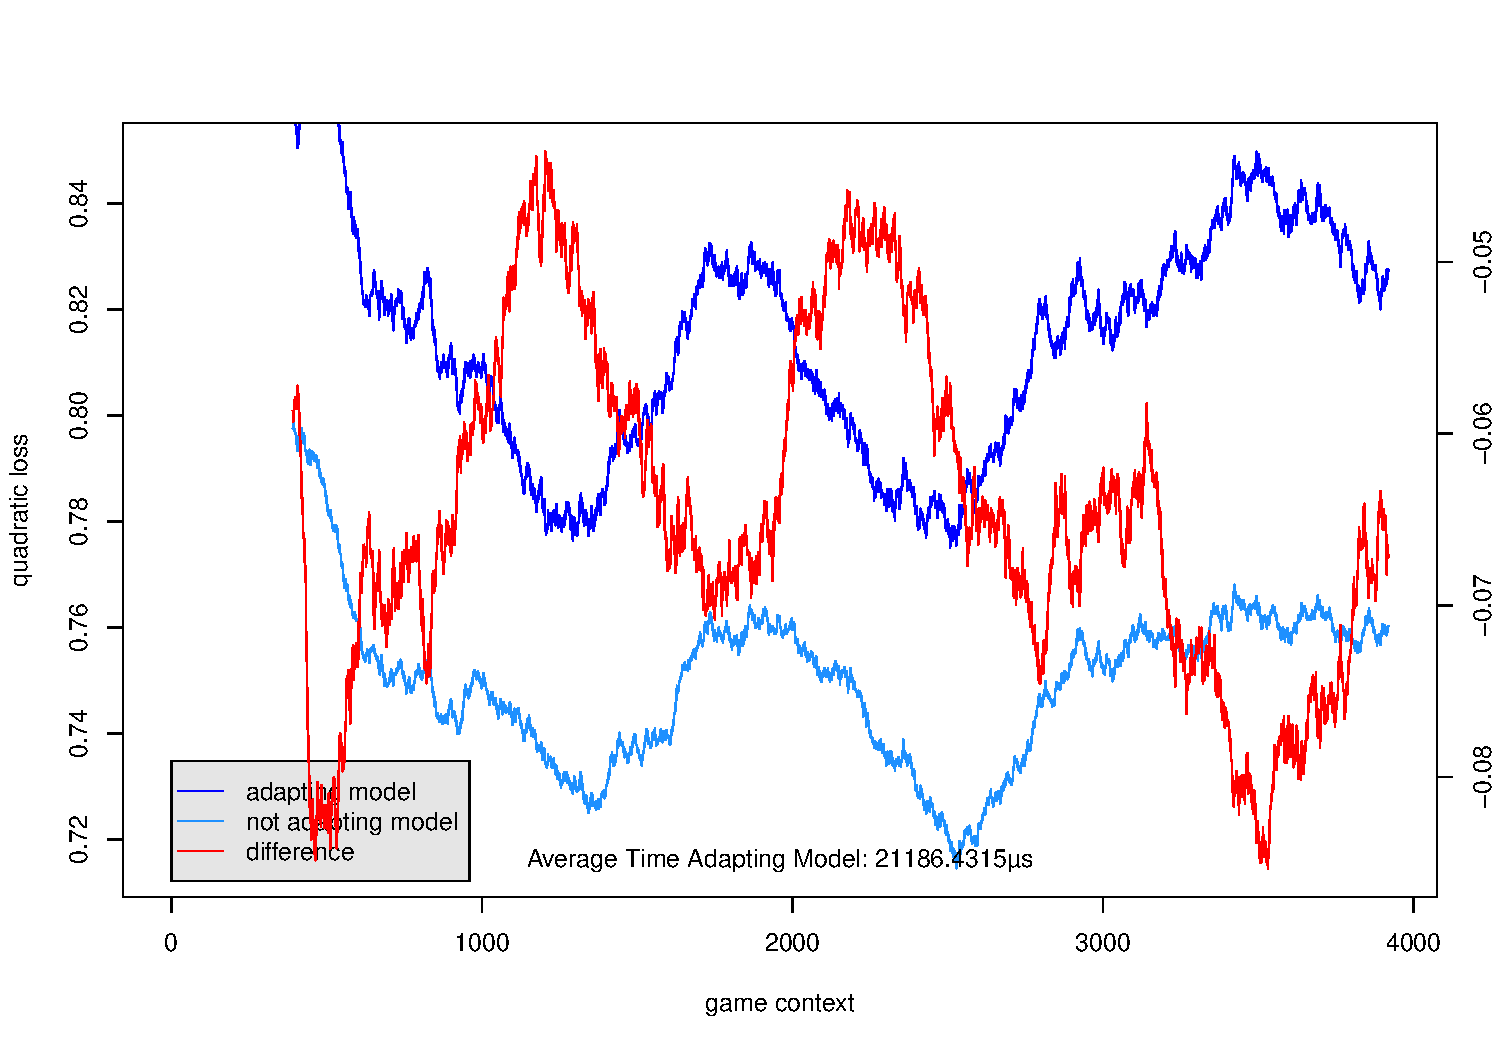
\includegraphics[scale=0.275]{section05-modelimpl/figures/MOANaiveBayes-HyperboreanNL-Eqm-action-quadratic}
}
\subfigure[Model of HyperboreanNL-Eqm: Correctly Predicted]{
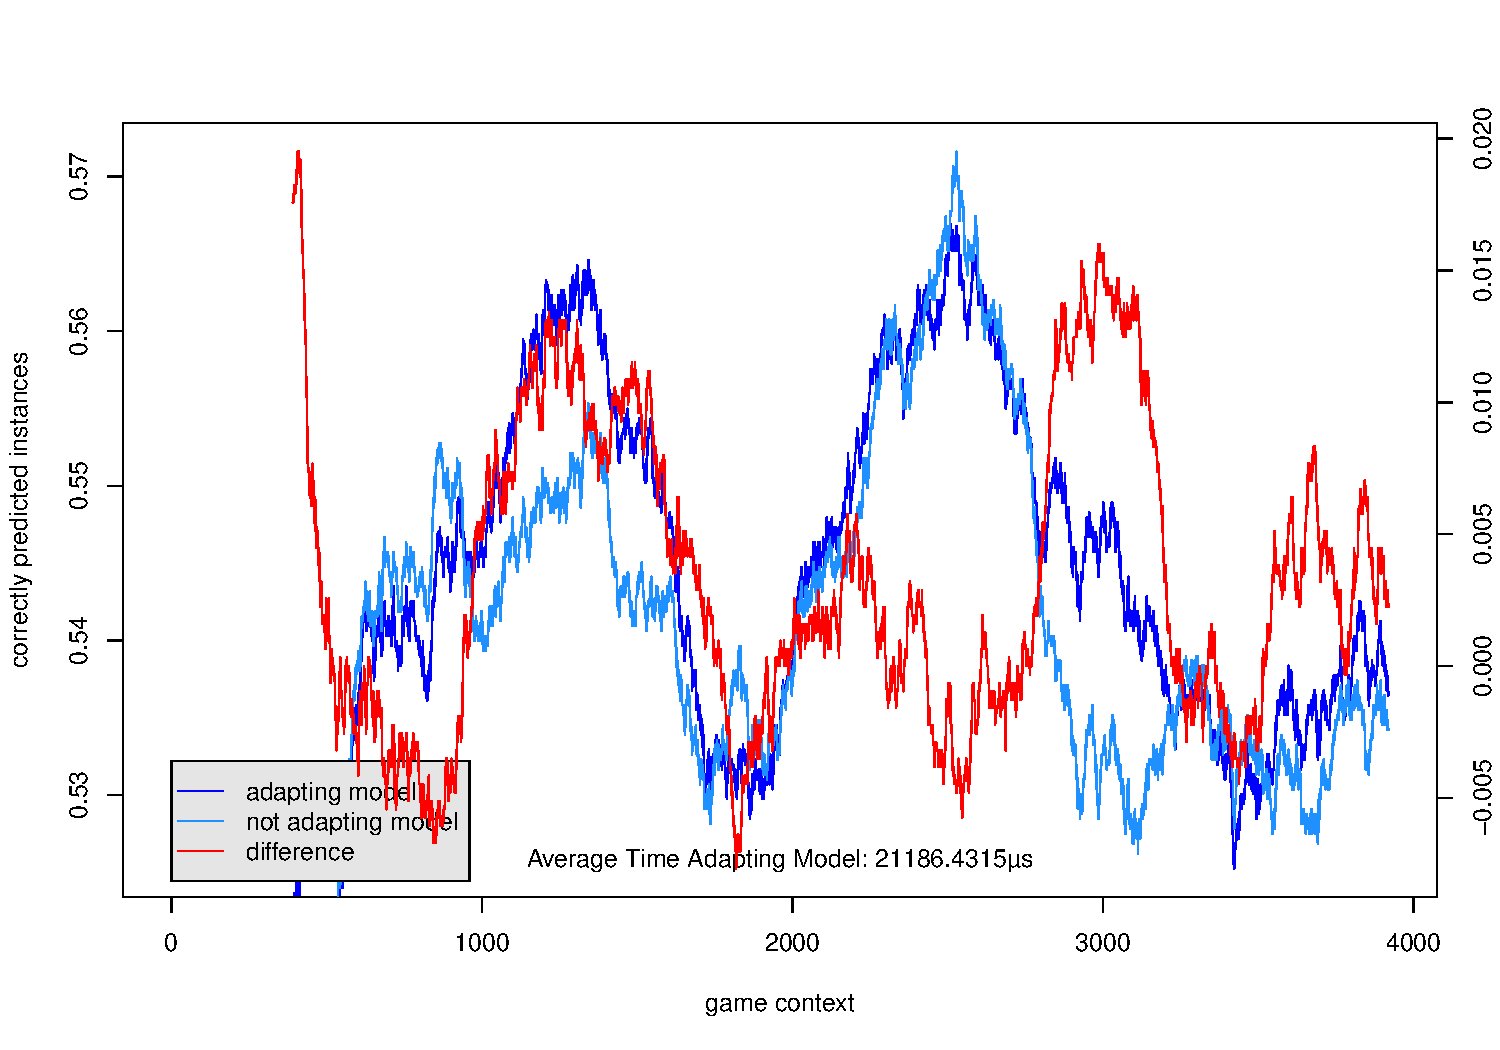
\includegraphics[scale=0.275]{section05-modelimpl/figures/MOANaiveBayes-HyperboreanNL-Eqm-action-correctly}
}

\subfigure[Model of HyperboreanNL-BR: Quadratic Loss]{
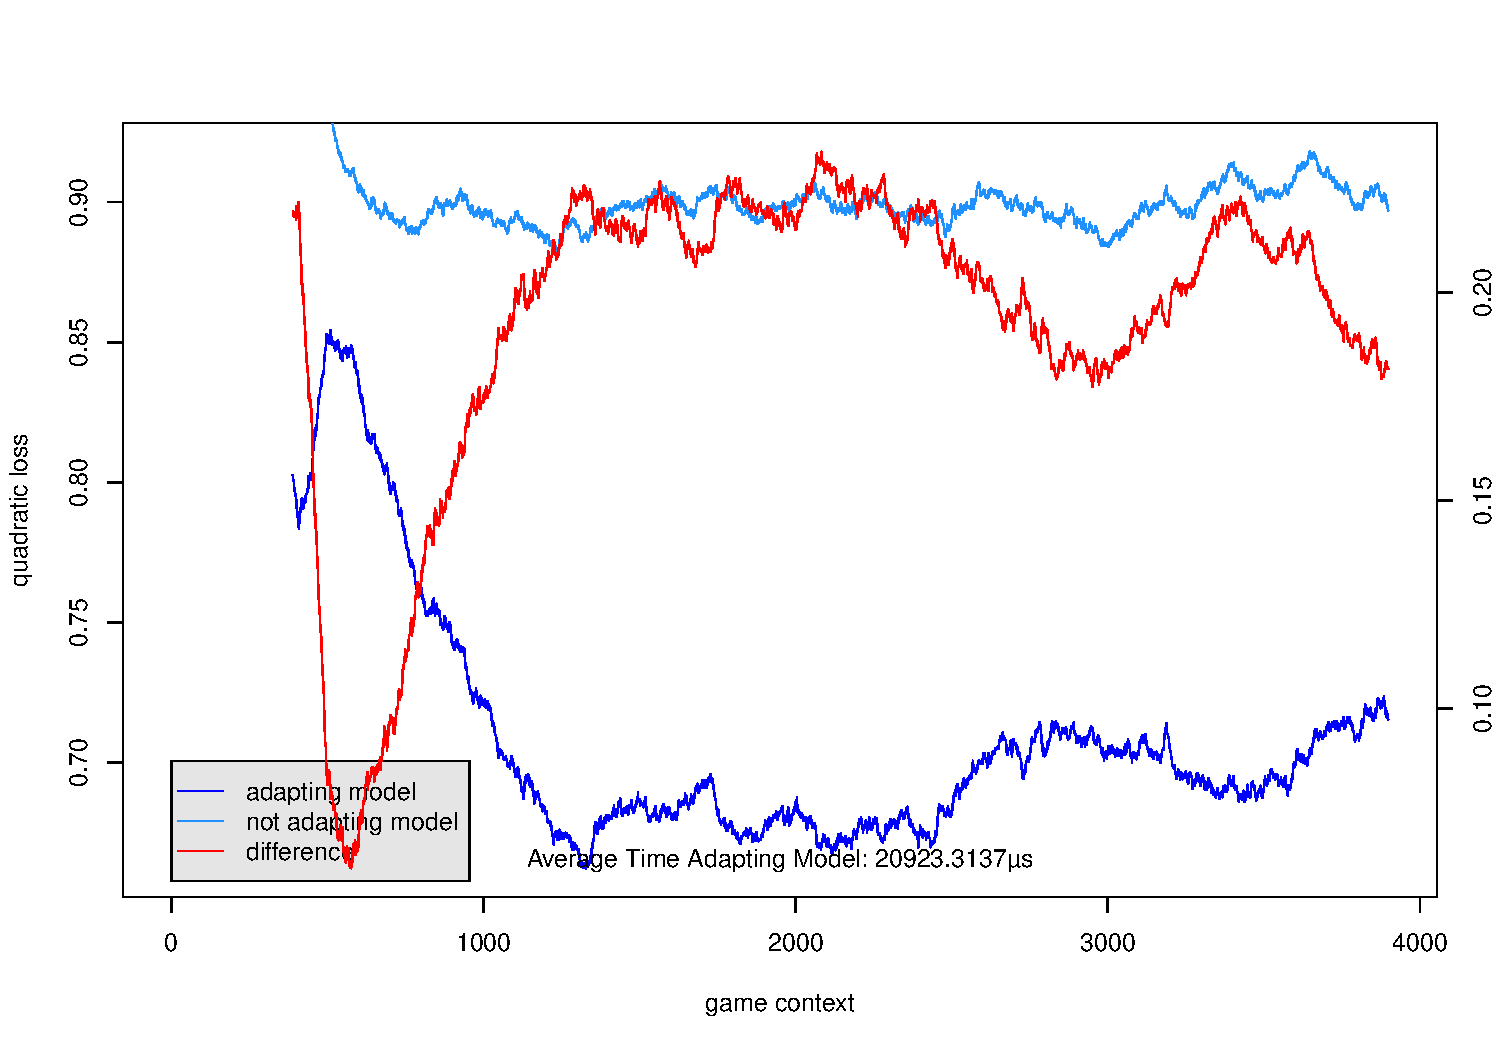
\includegraphics[scale=0.275]{section05-modelimpl/figures/MOANaiveBayes-HyperboreanNL-BR-action-quadratic}
}
\subfigure[Model of HyperboreanNL-BR: Correctly Predicted]{
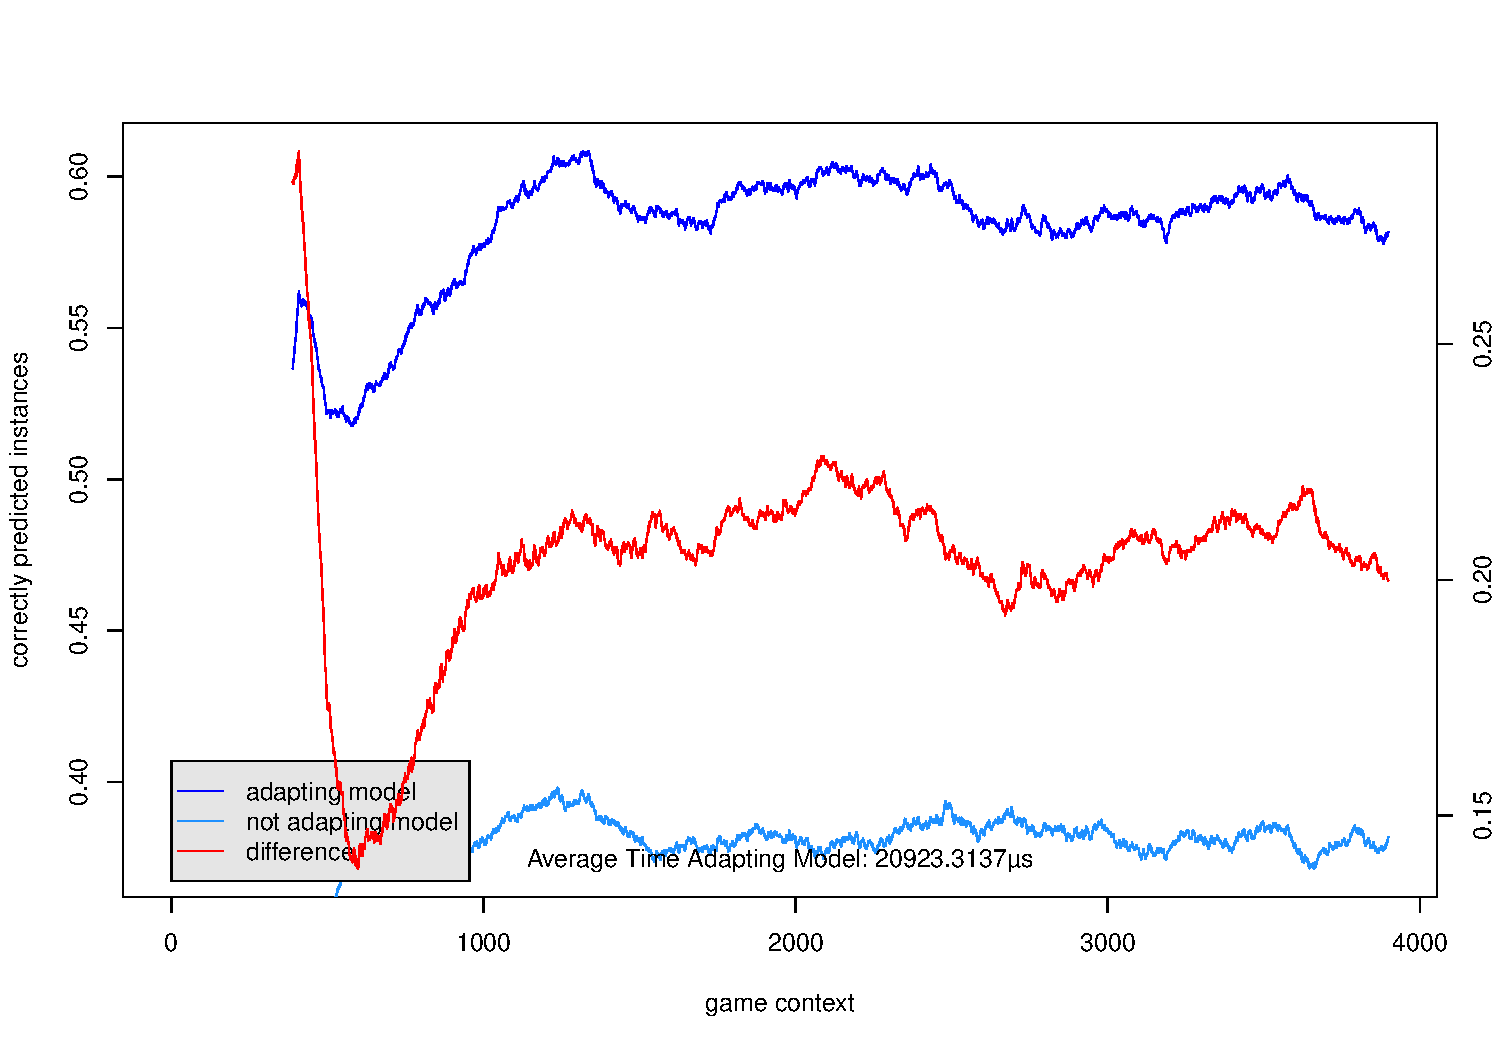
\includegraphics[scale=0.275]{section05-modelimpl/figures/MOANaiveBayes-HyperboreanNL-BR-action-correctly}
}

\subfigure[Model of BluffBot4: Quadratic Loss]{
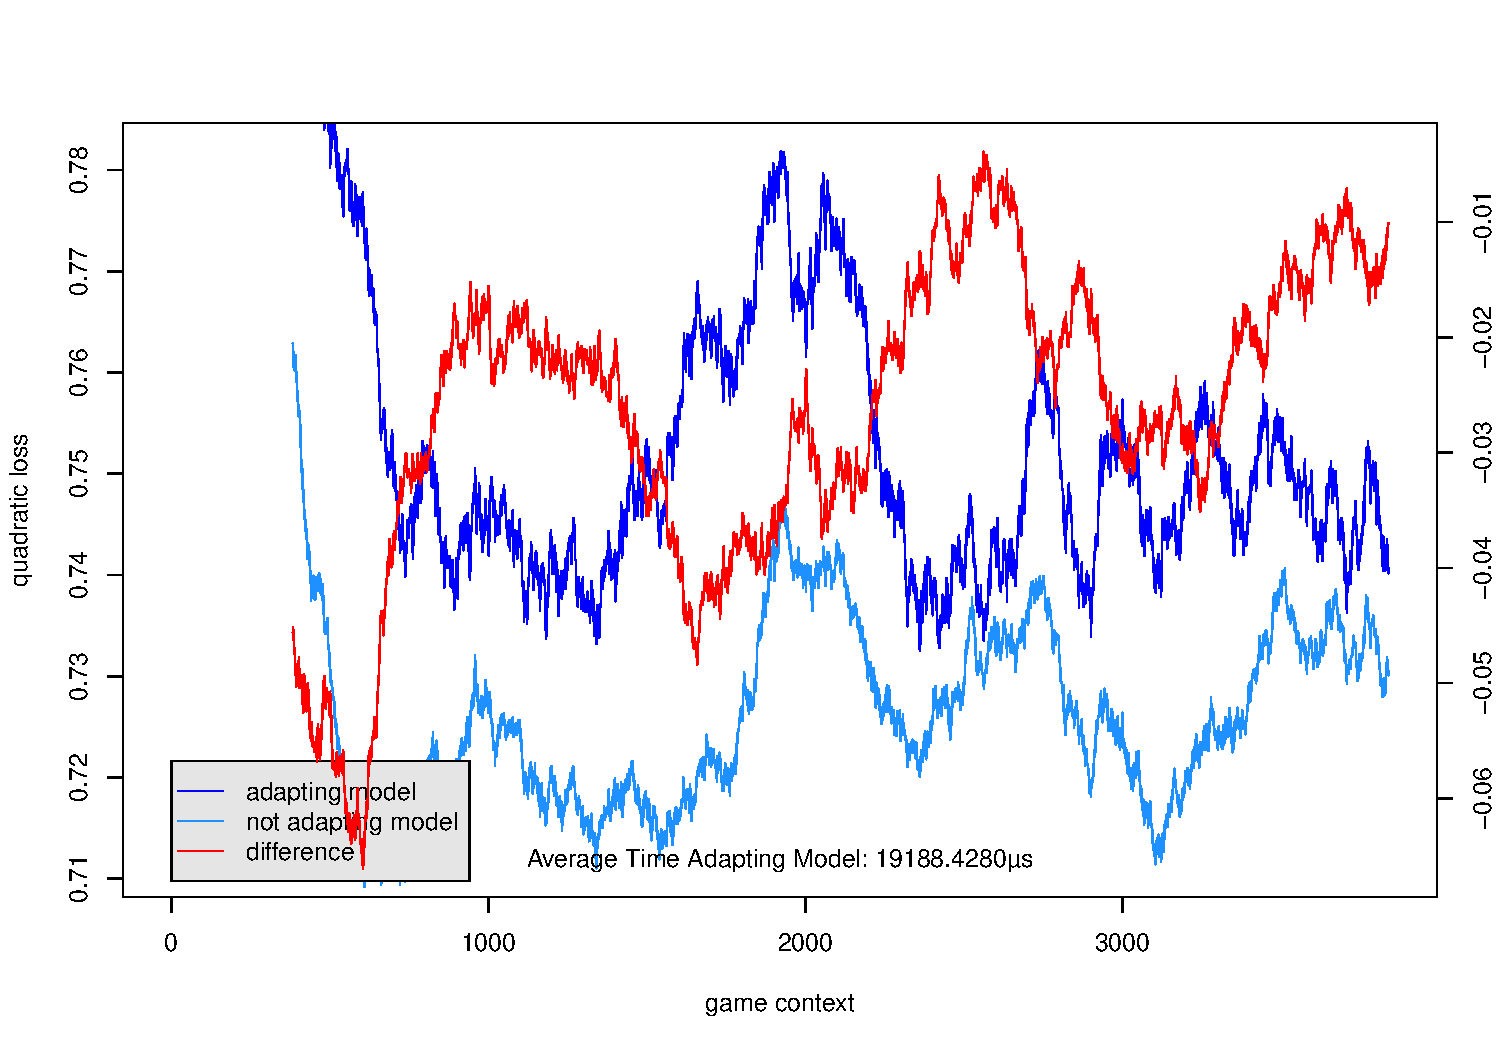
\includegraphics[scale=0.275]{section05-modelimpl/figures/MOANaiveBayes-BluffBot4-action-quadratic}
}
\subfigure[Model of BluffBot4: Correctly Predicted]{
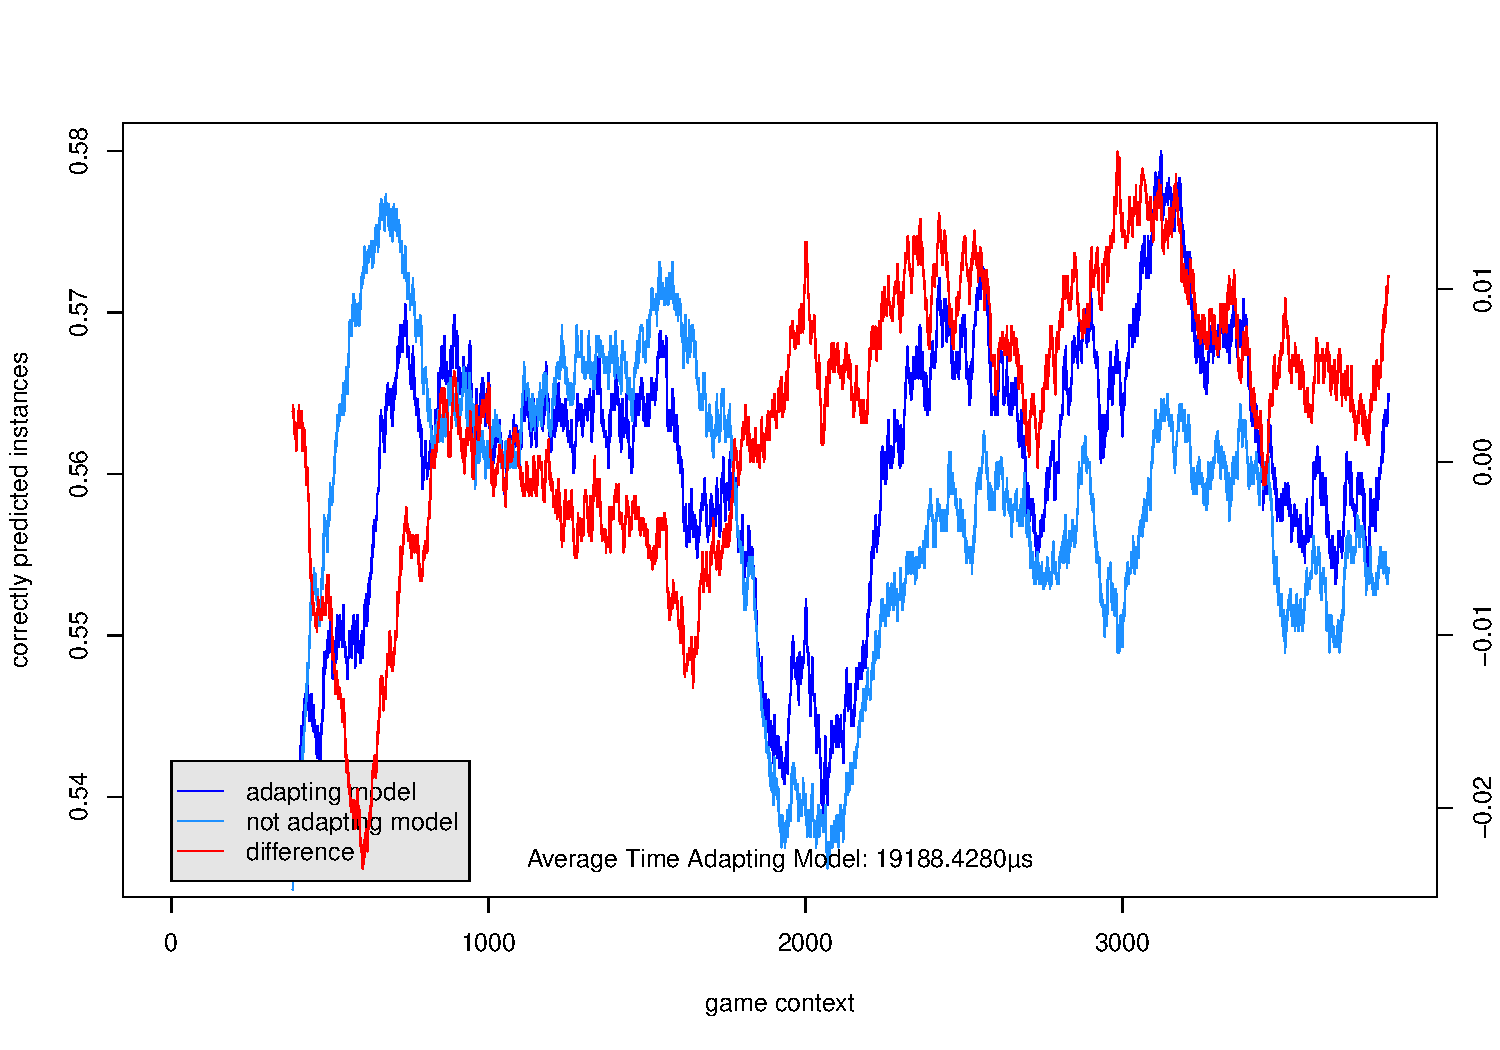
\includegraphics[scale=0.275]{section05-modelimpl/figures/MOANaiveBayes-BluffBot4-action-correctly}
}

\caption{Action Prediction: Naive Bayes}
\label{fig:MOANaiveBayes-action}
\end{figure}




\newpage
\subsection{Performance in Action Prediction: Online Backpropagation}
\begin{figure}[h!]
\centering

\subfigure[Model of HyperboreanNL-Eqm: Quadratic Loss]{
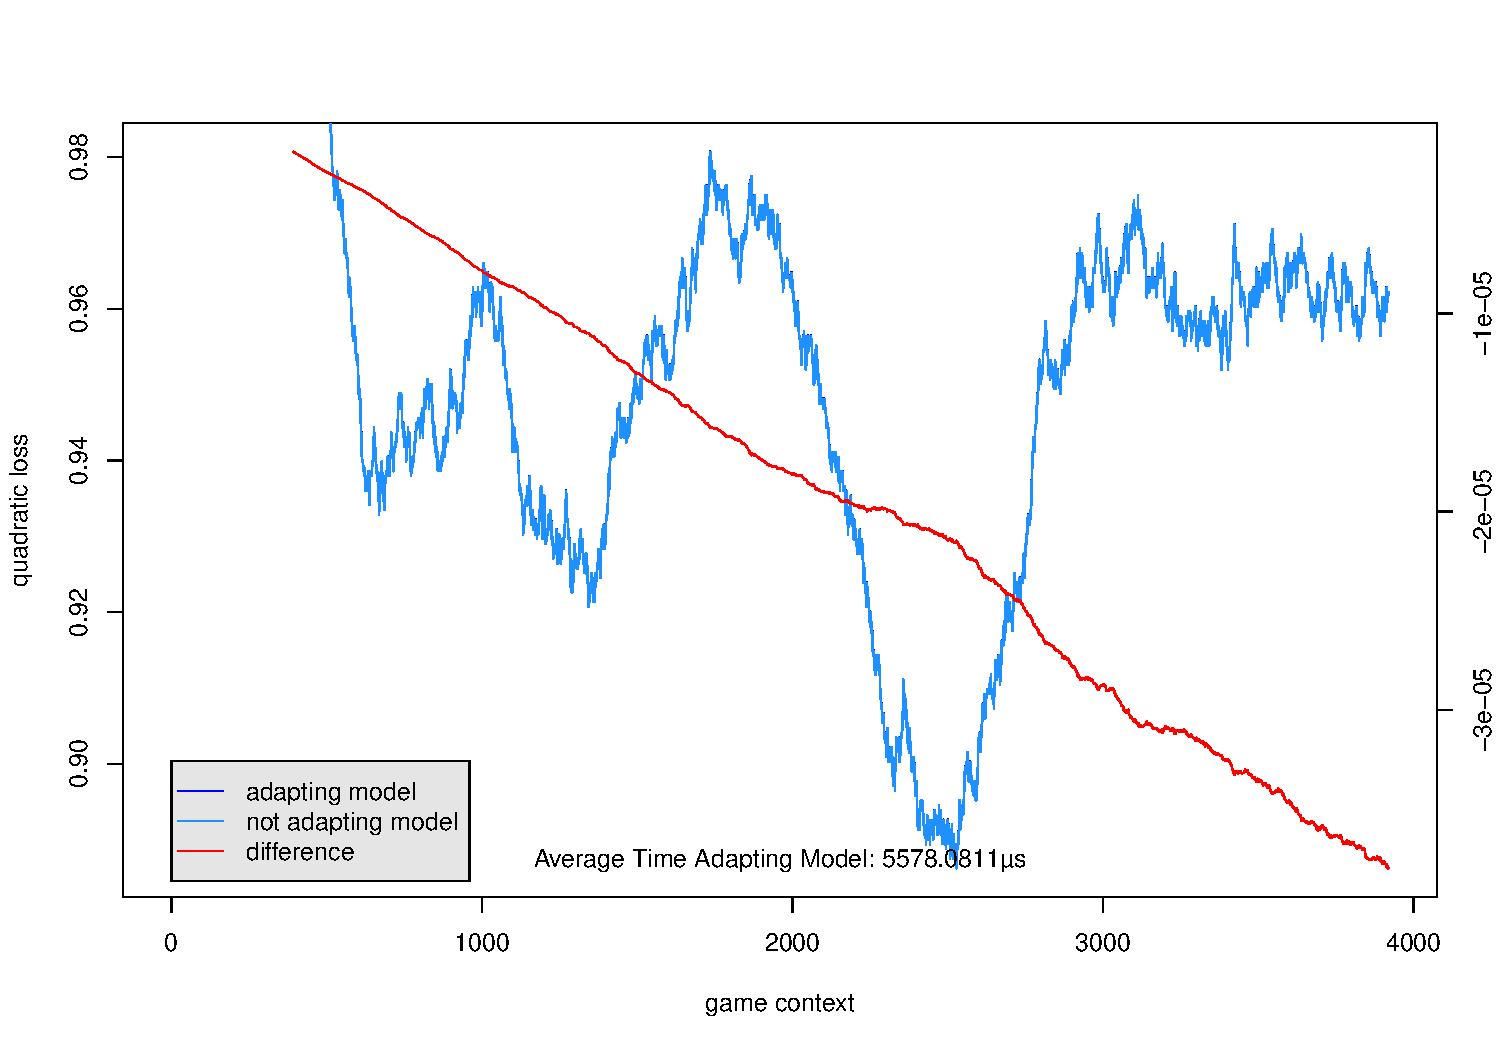
\includegraphics[scale=0.275]{section05-modelimpl/figures/OnlineBackpropagation-HyperboreanNL-Eqm-action-quadratic}
}
\subfigure[Model of HyperboreanNL-Eqm: Correctly Predicted]{
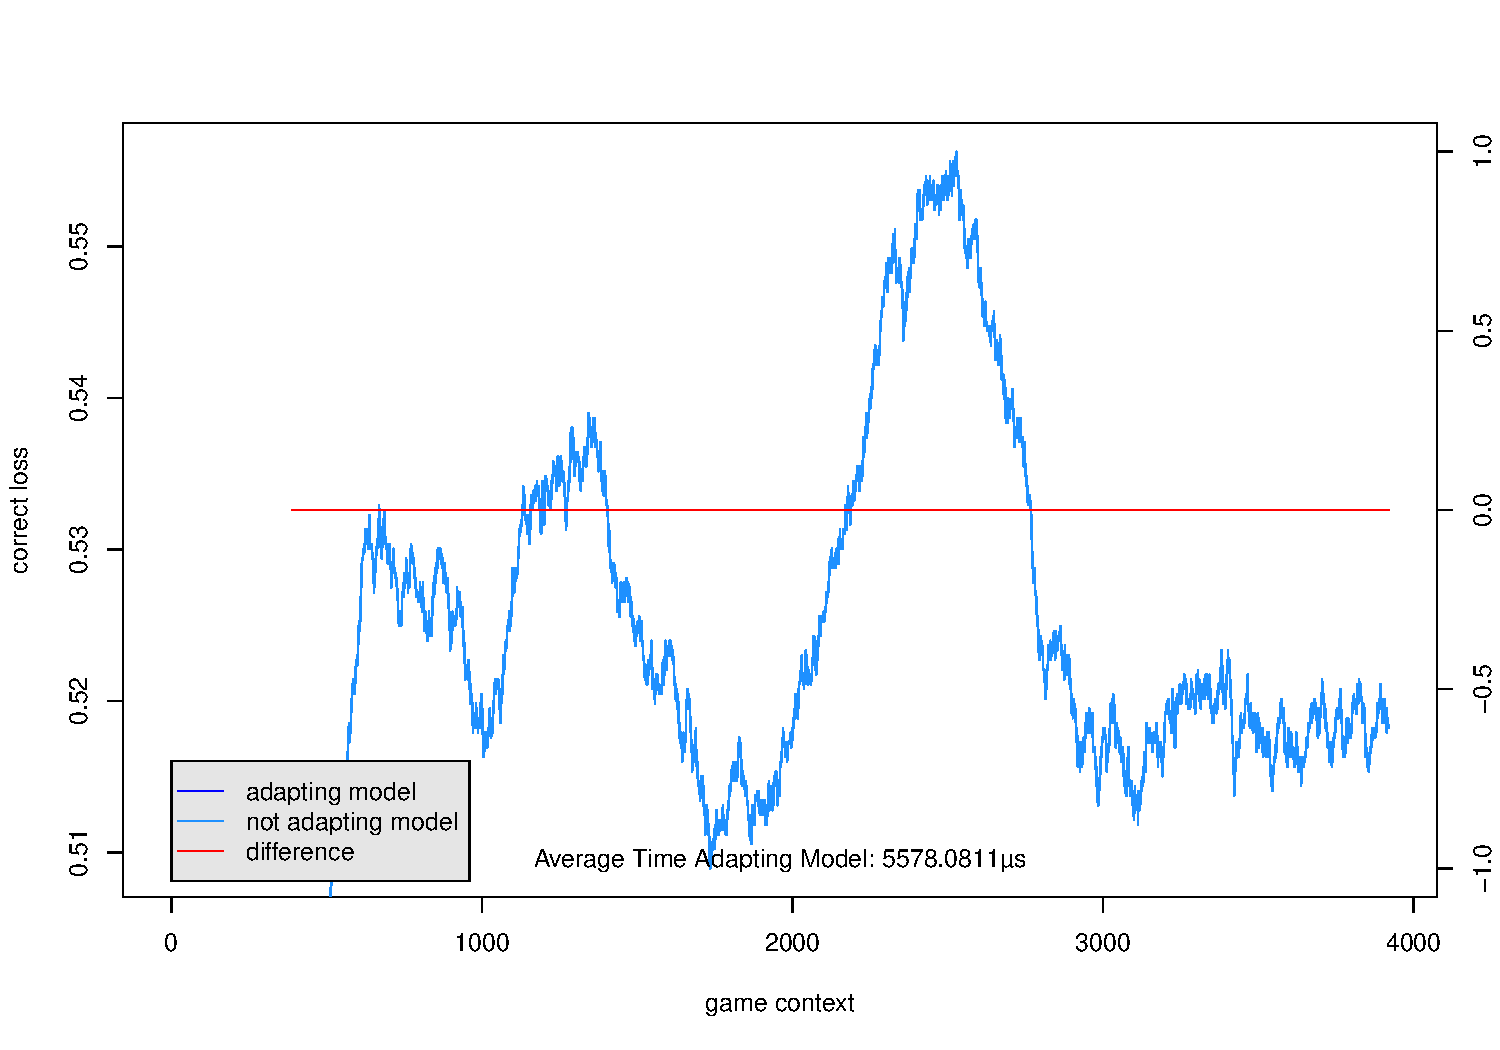
\includegraphics[scale=0.275]{section05-modelimpl/figures/OnlineBackpropagation-HyperboreanNL-Eqm-action-correctly}
}

\subfigure[Model of HyperboreanNL-BR: Quadratic Loss]{
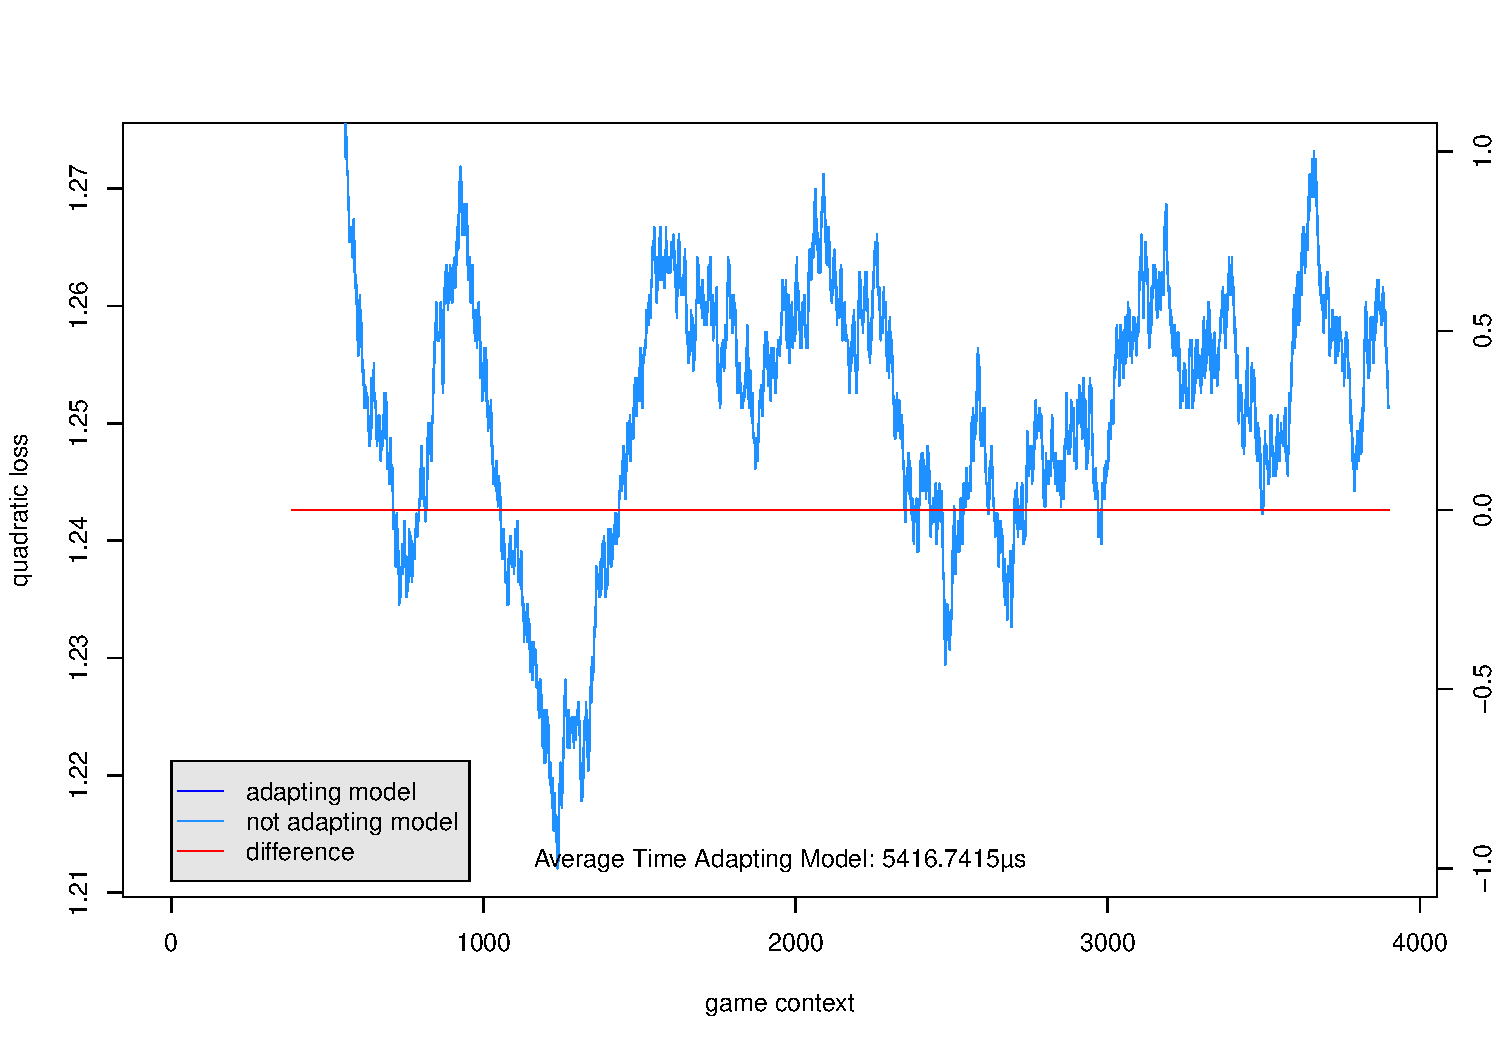
\includegraphics[scale=0.275]{section05-modelimpl/figures/OnlineBackpropagation-HyperboreanNL-BR-action-quadratic}
}
\subfigure[Model of HyperboreanNL-BR: Correctly Predicted]{
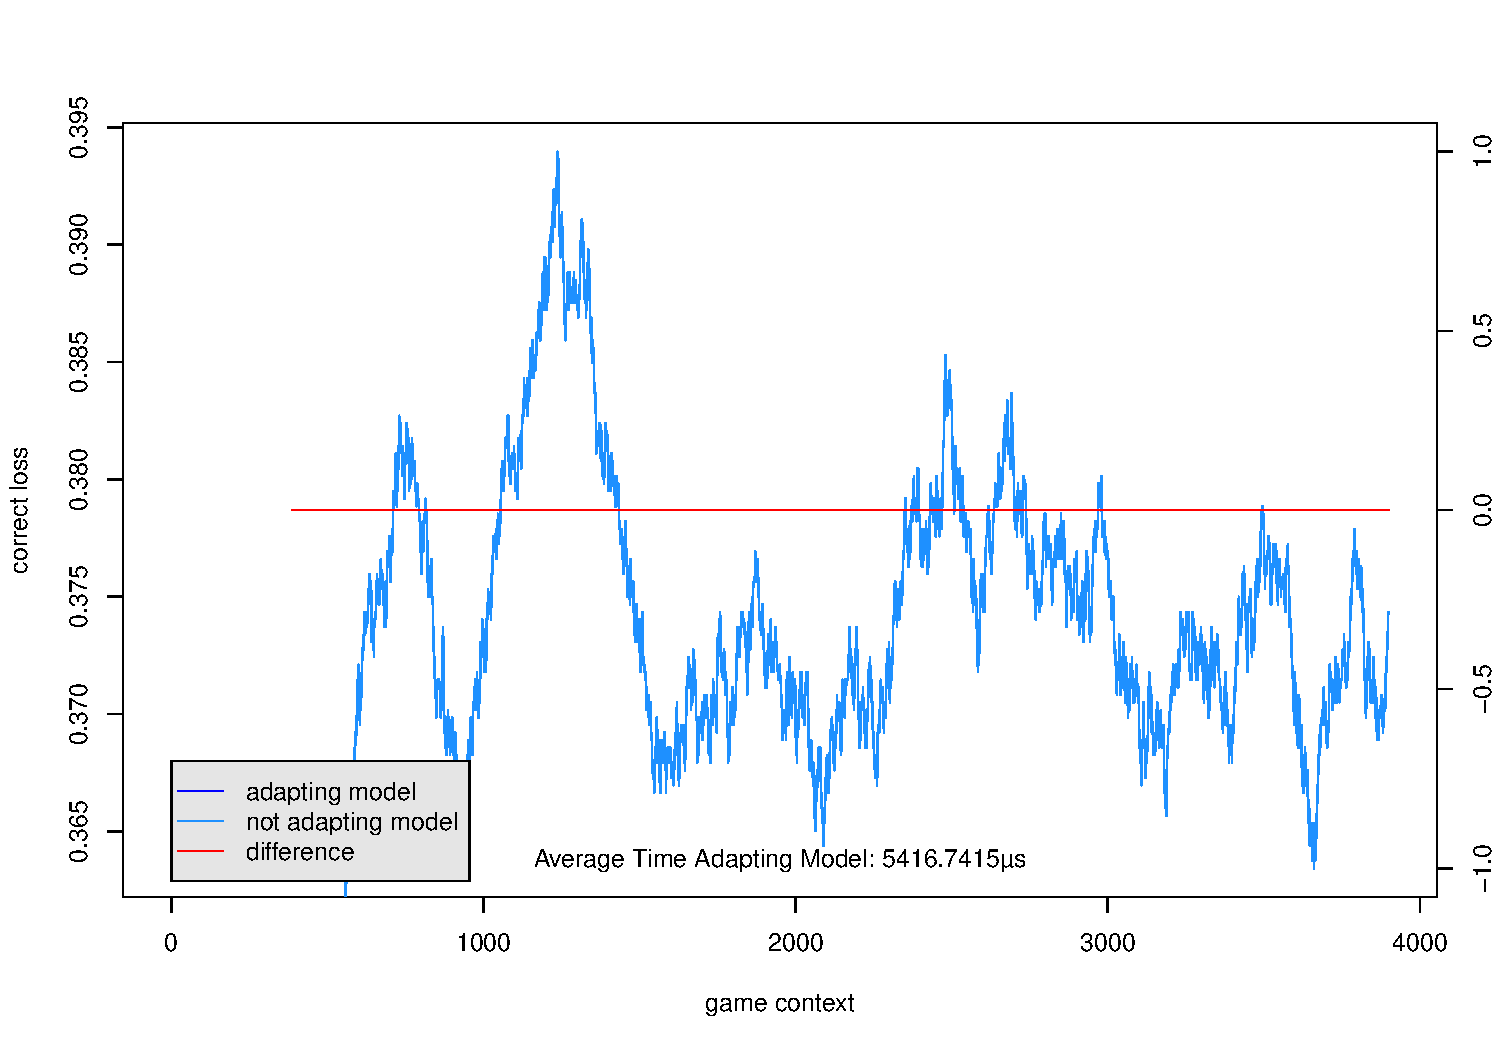
\includegraphics[scale=0.275]{section05-modelimpl/figures/OnlineBackpropagation-HyperboreanNL-BR-action-correctly}
}

\subfigure[Model of BluffBot4: Quadratic Loss]{
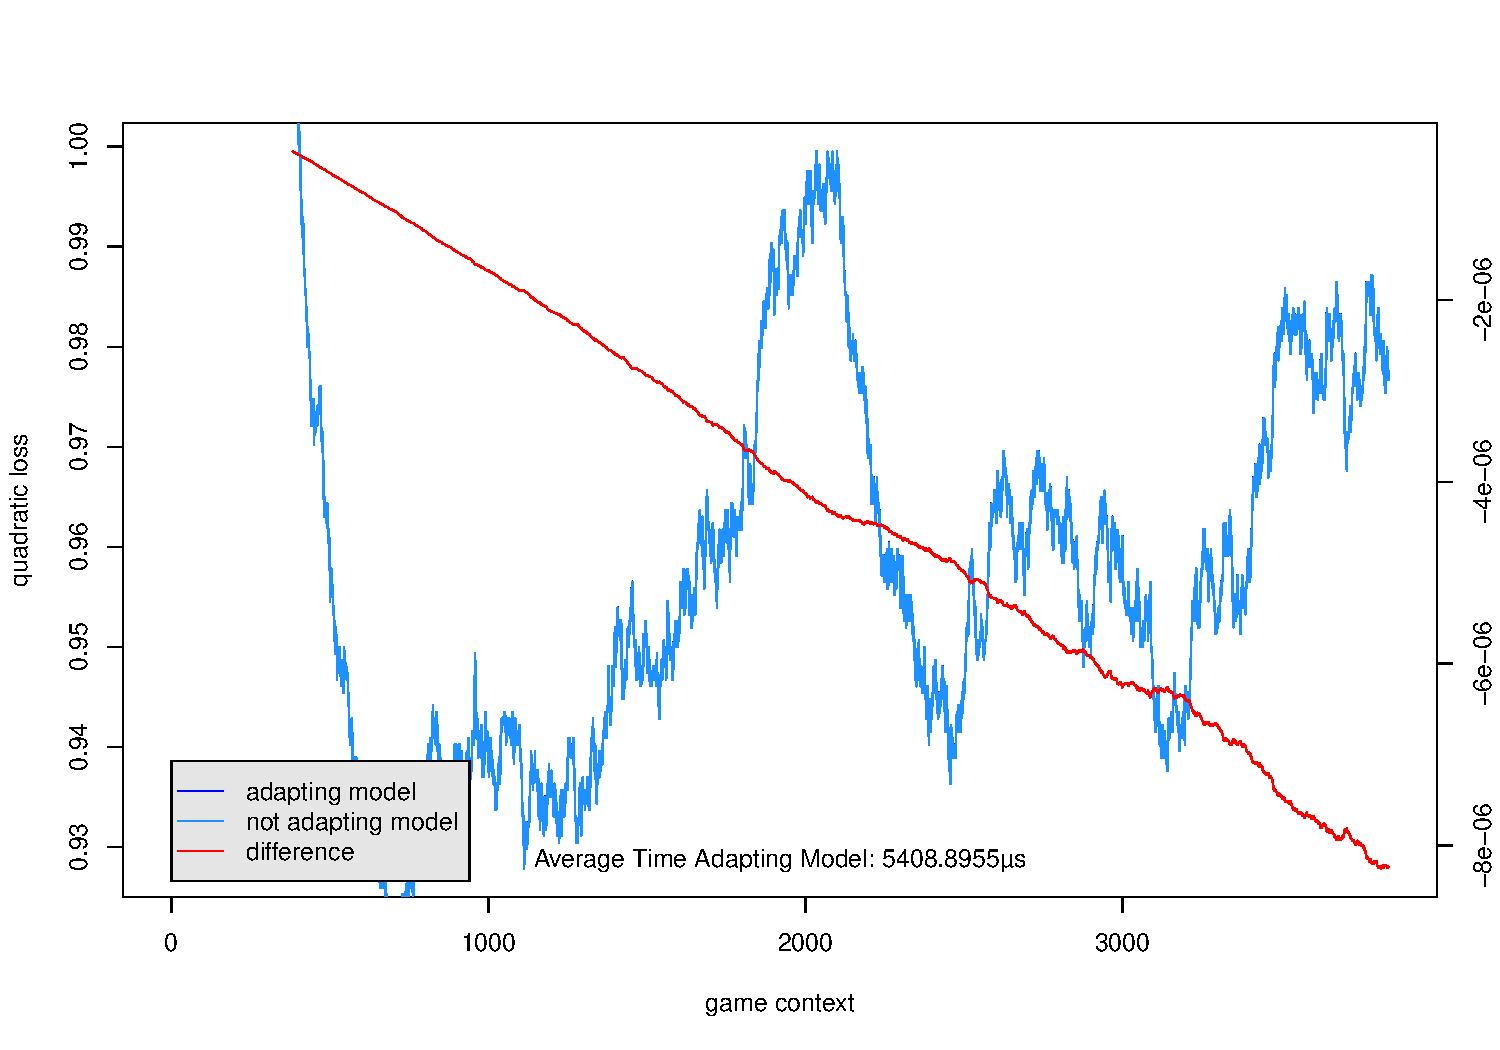
\includegraphics[scale=0.275]{section05-modelimpl/figures/OnlineBackpropagation-BluffBot4-action-quadratic}
}
\subfigure[Model of BluffBot4: Correctly Predicted]{
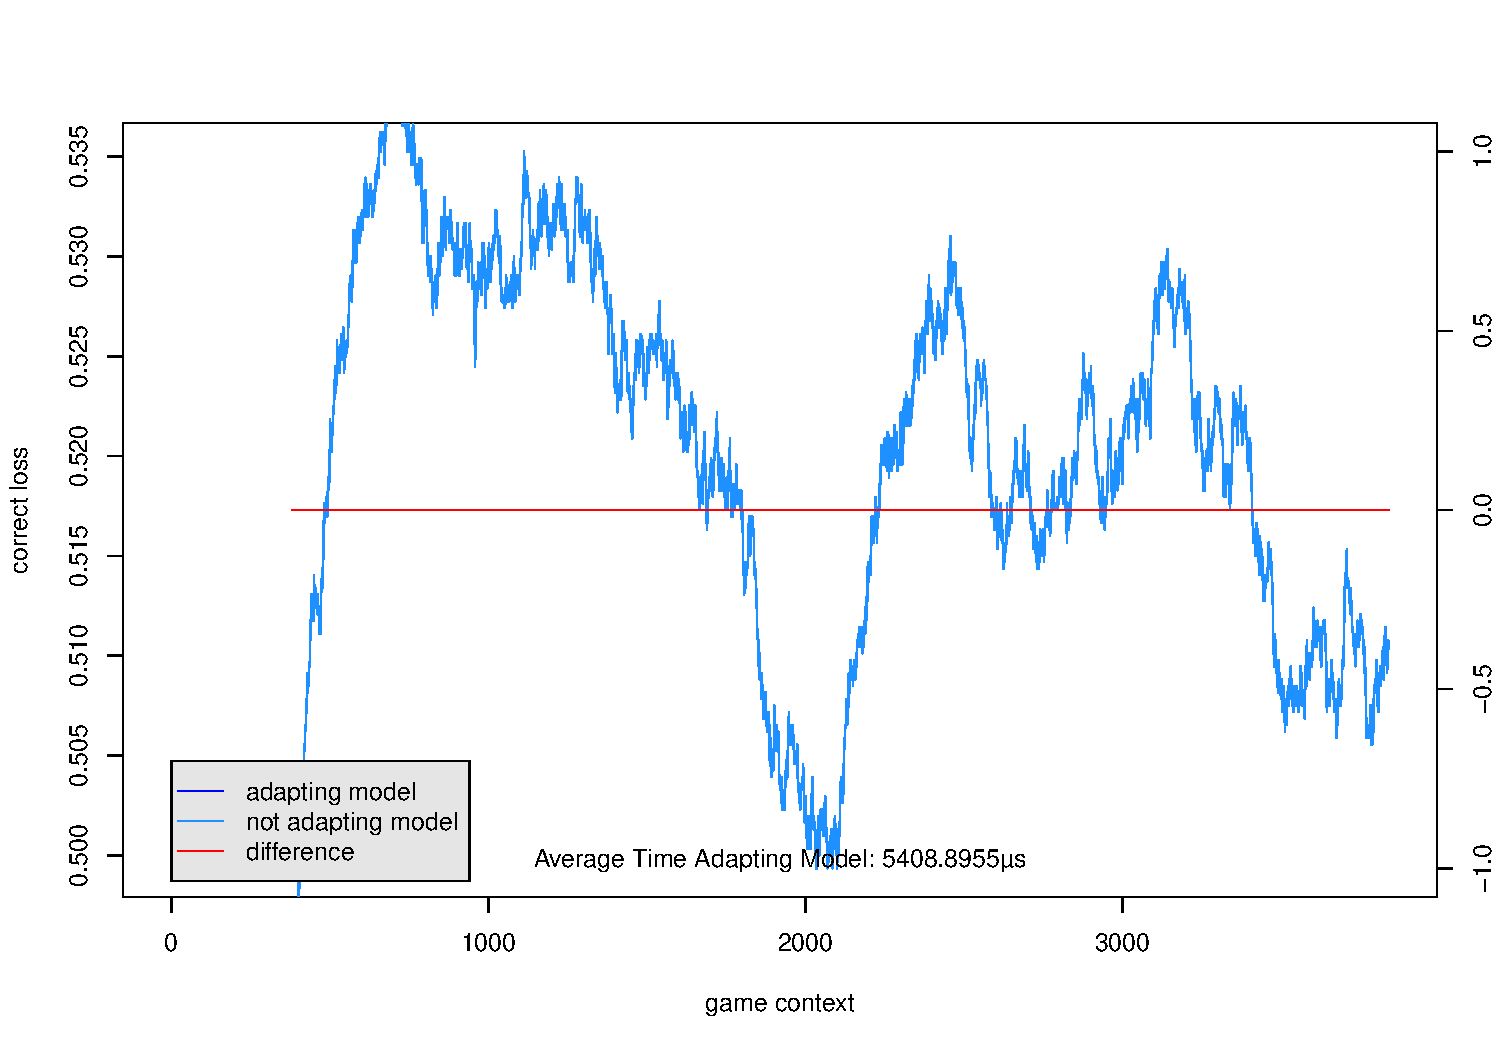
\includegraphics[scale=0.275]{section05-modelimpl/figures/OnlineBackpropagation-BluffBot4-action-correctly}
}

\caption{Action Prediction: Online Backpropagation}
\label{fig:OnlineBackpropagation-action}
\end{figure}


\newpage
\subsection{Performance in Action Prediction: Hoeffding Tree}
\begin{figure}[h!]
\centering

\subfigure[Model of HyperboreanNL-Eqm: Quadratic Loss]{
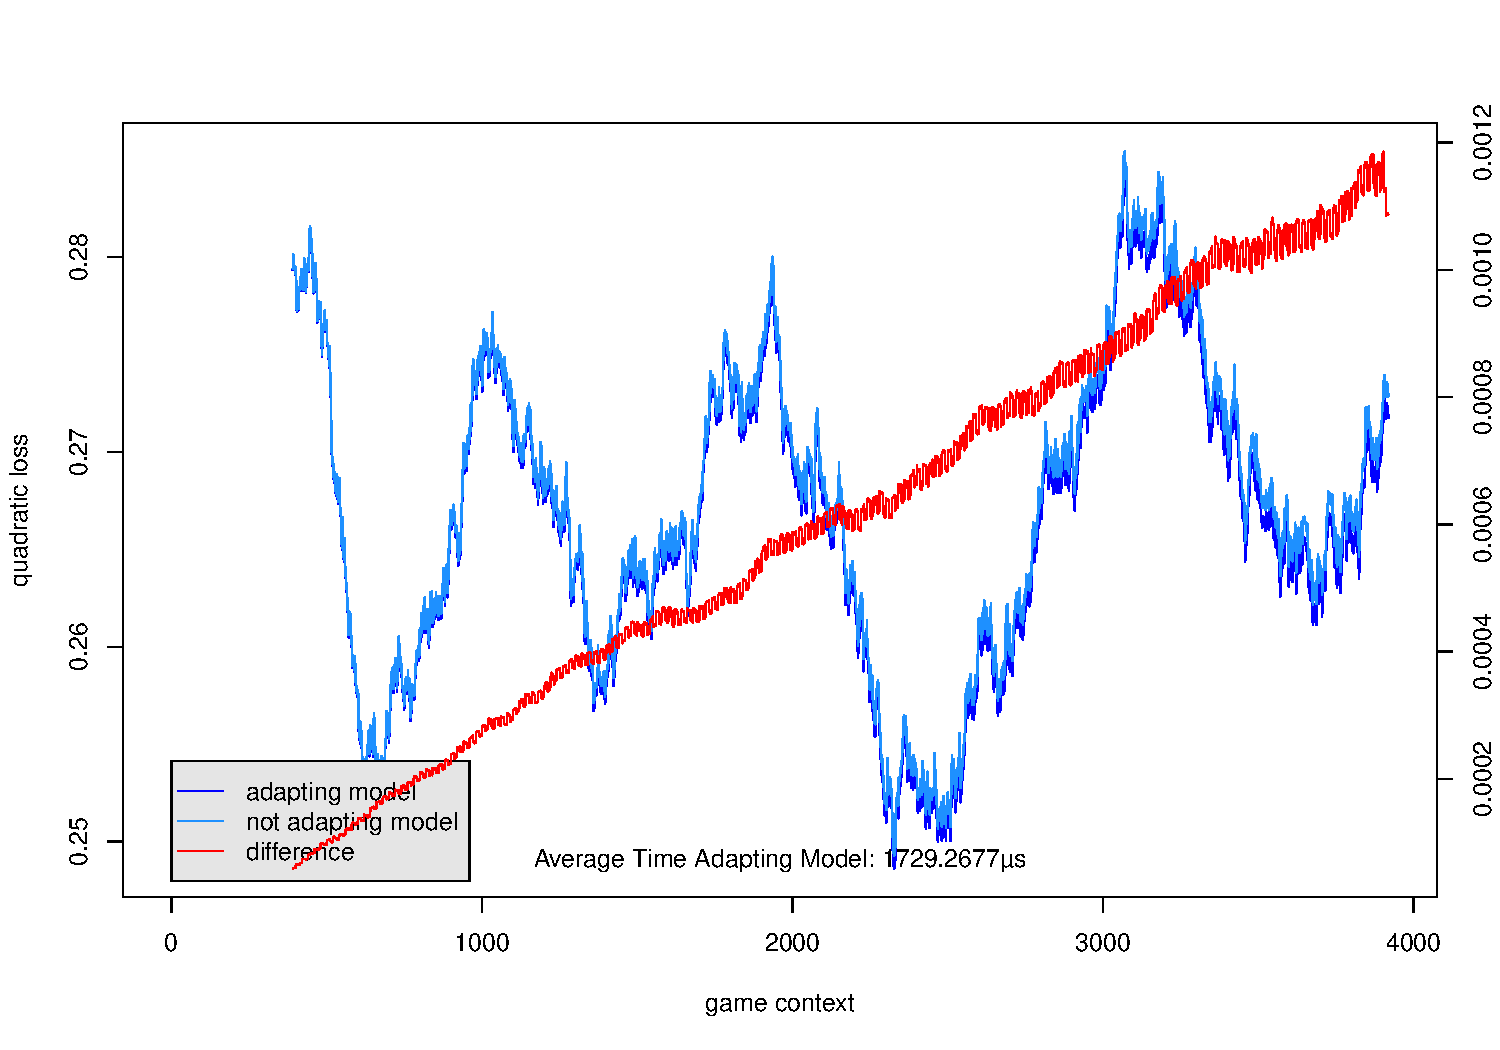
\includegraphics[scale=0.275]{section05-modelimpl/figures/HoeffdingTree-HyperboreanNL-Eqm-action-quadratic}
}
\subfigure[Model of HyperboreanNL-Eqm: Correctly Predicted]{
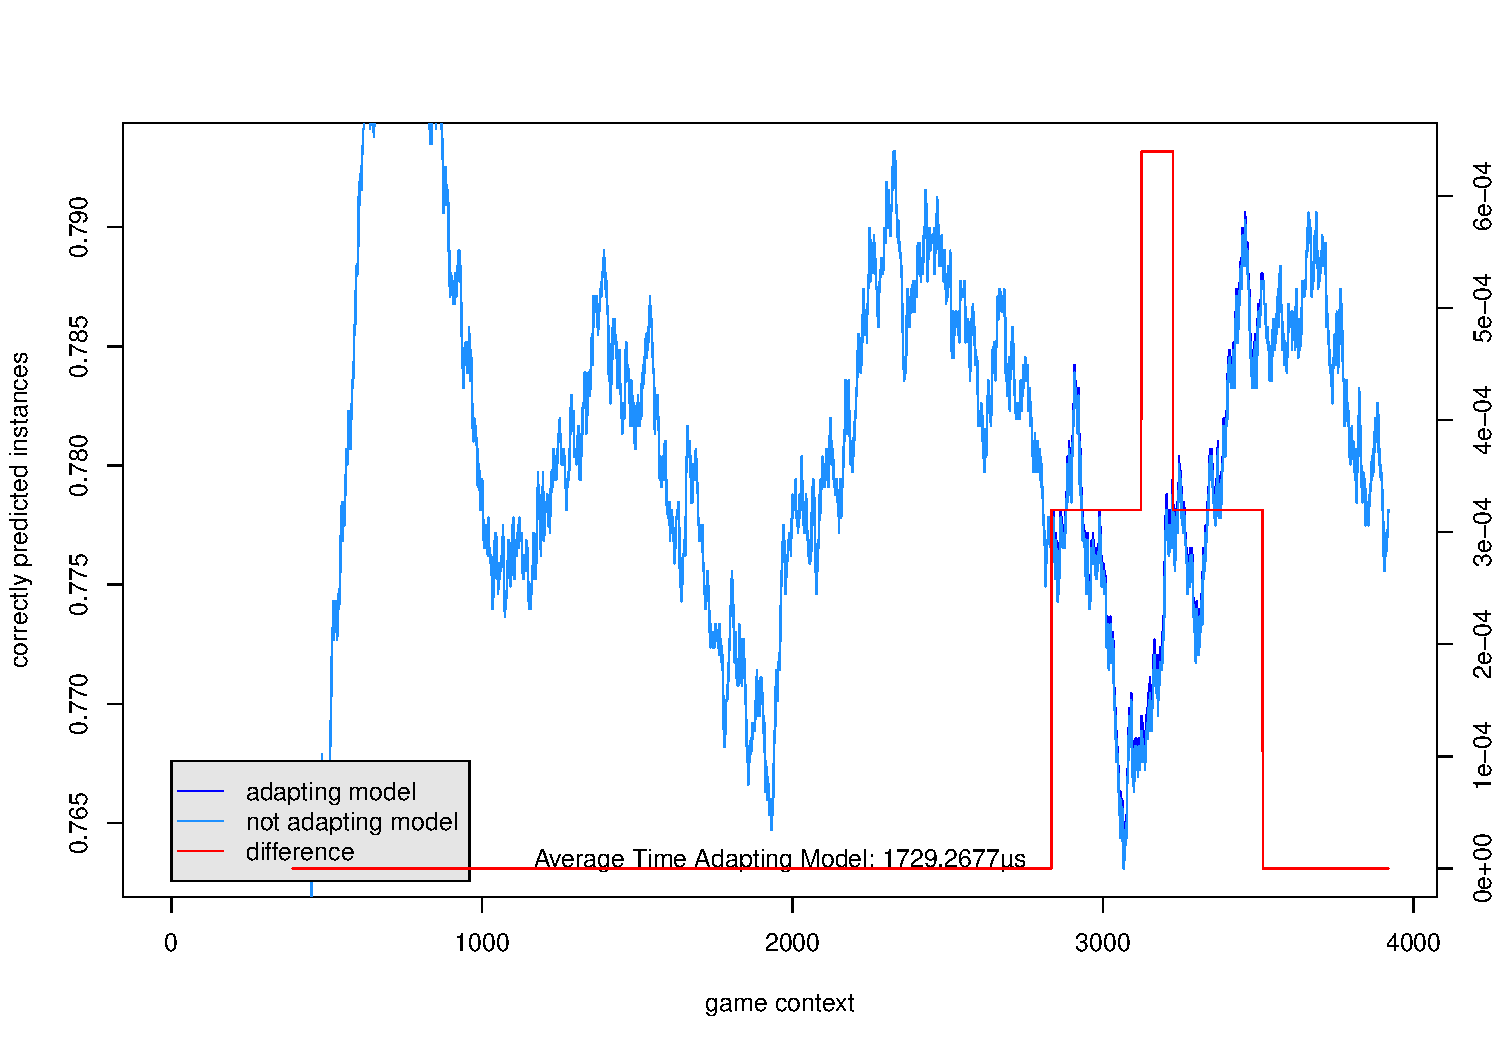
\includegraphics[scale=0.275]{section05-modelimpl/figures/HoeffdingTree-HyperboreanNL-Eqm-action-correctly}
}

\subfigure[Model of HyperboreanNL-BR: Quadratic Loss]{
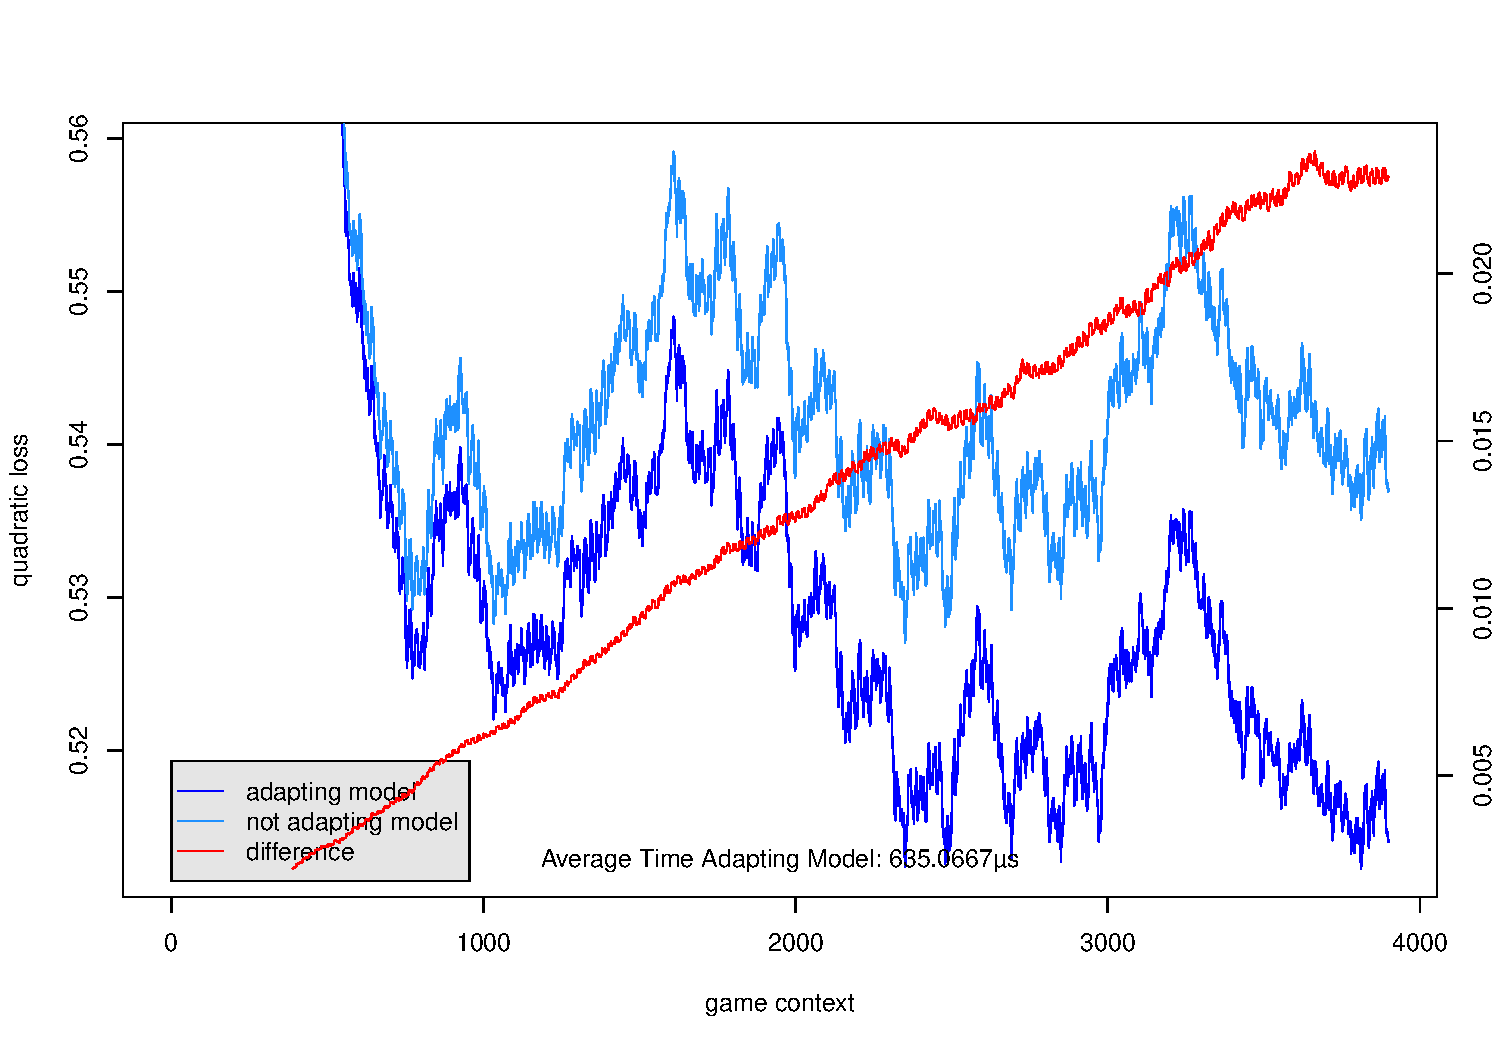
\includegraphics[scale=0.275]{section05-modelimpl/figures/HoeffdingTree-HyperboreanNL-BR-action-quadratic}
}
\subfigure[Model of HyperboreanNL-BR: Correctly Predicted]{
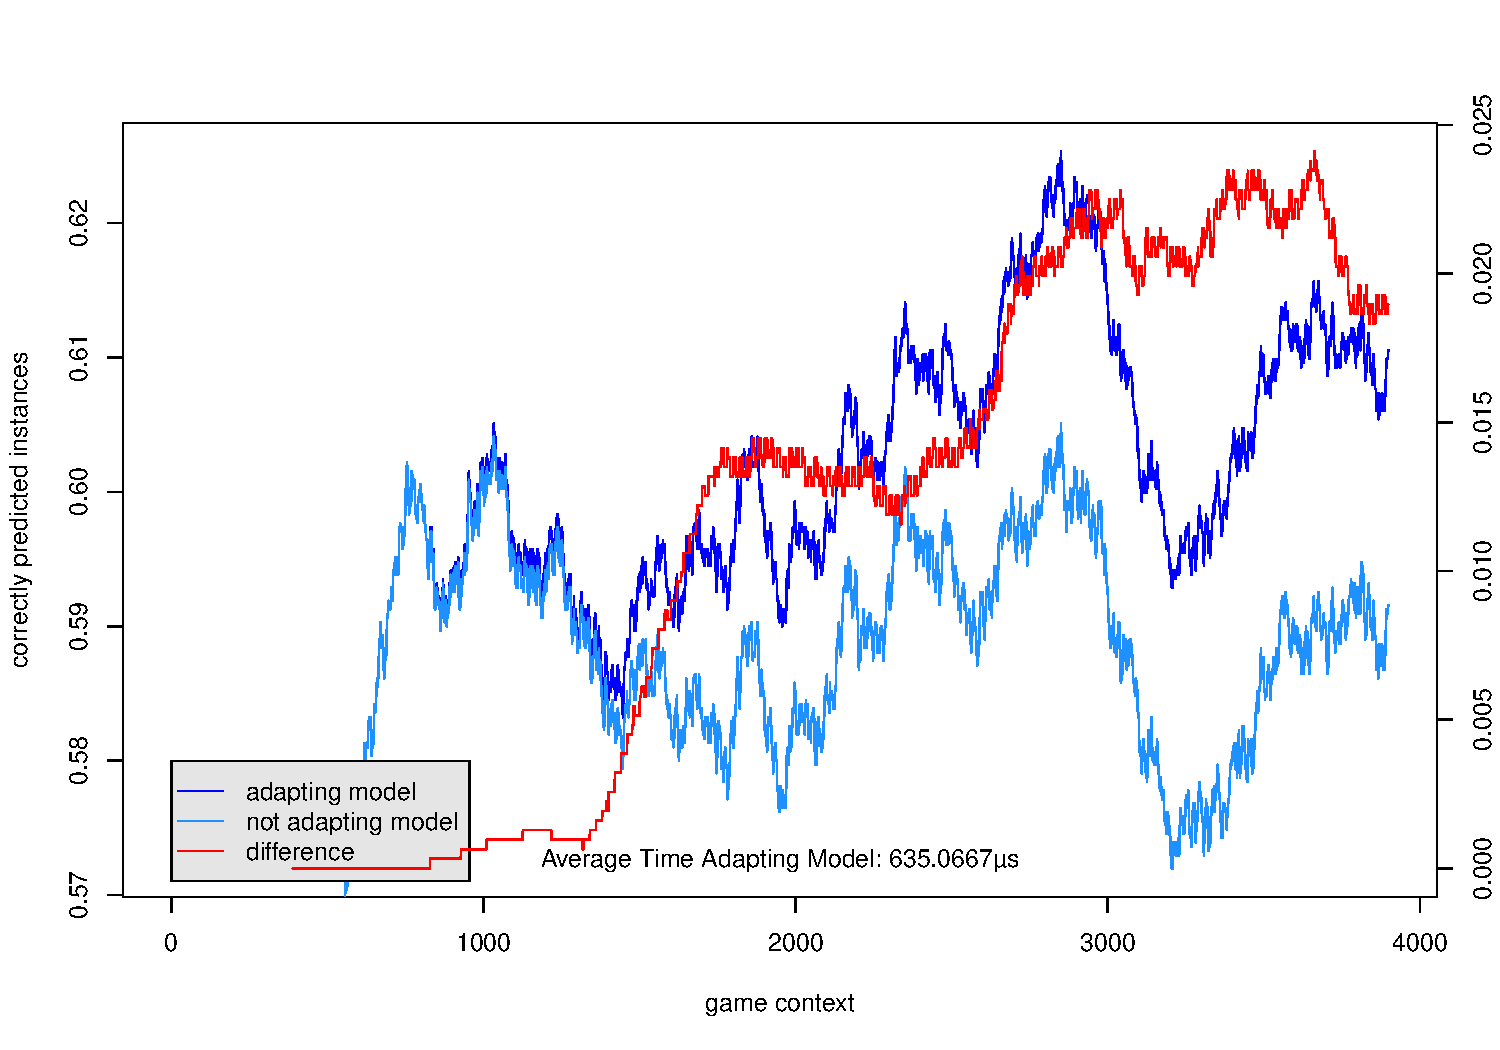
\includegraphics[scale=0.275]{section05-modelimpl/figures/HoeffdingTree-HyperboreanNL-BR-action-correctly}
}

\subfigure[Model of BluffBot4: Quadratic Loss]{
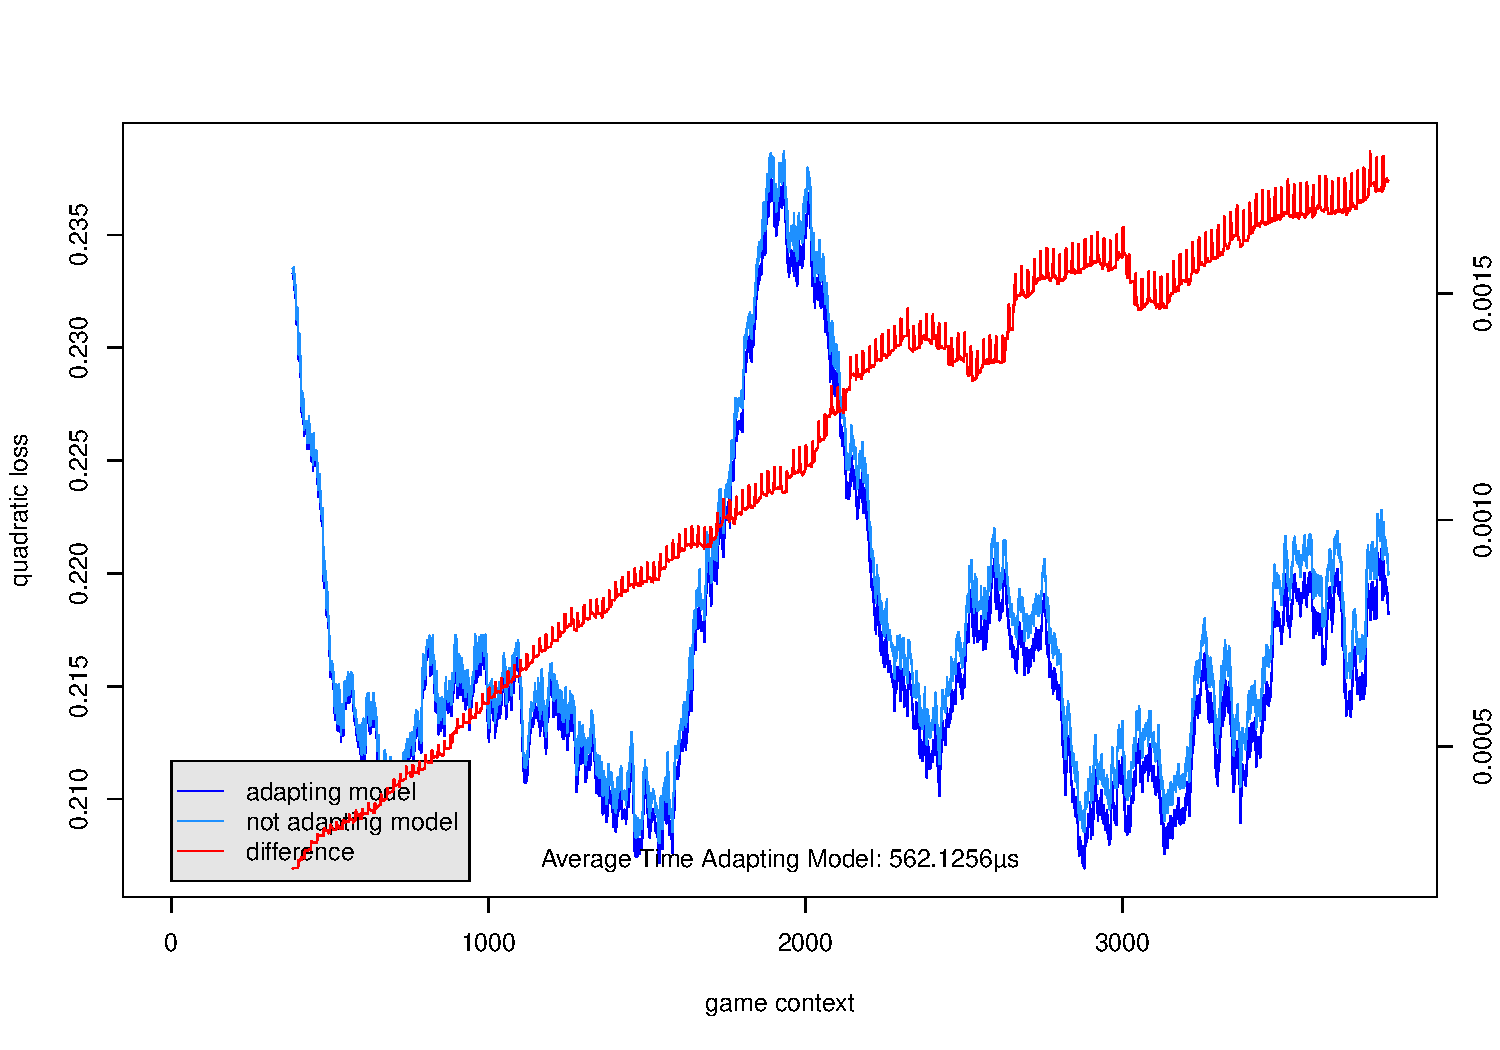
\includegraphics[scale=0.275]{section05-modelimpl/figures/HoeffdingTree-BluffBot4-action-quadratic}
}
\subfigure[Model of BluffBot4: Correctly Predicted]{
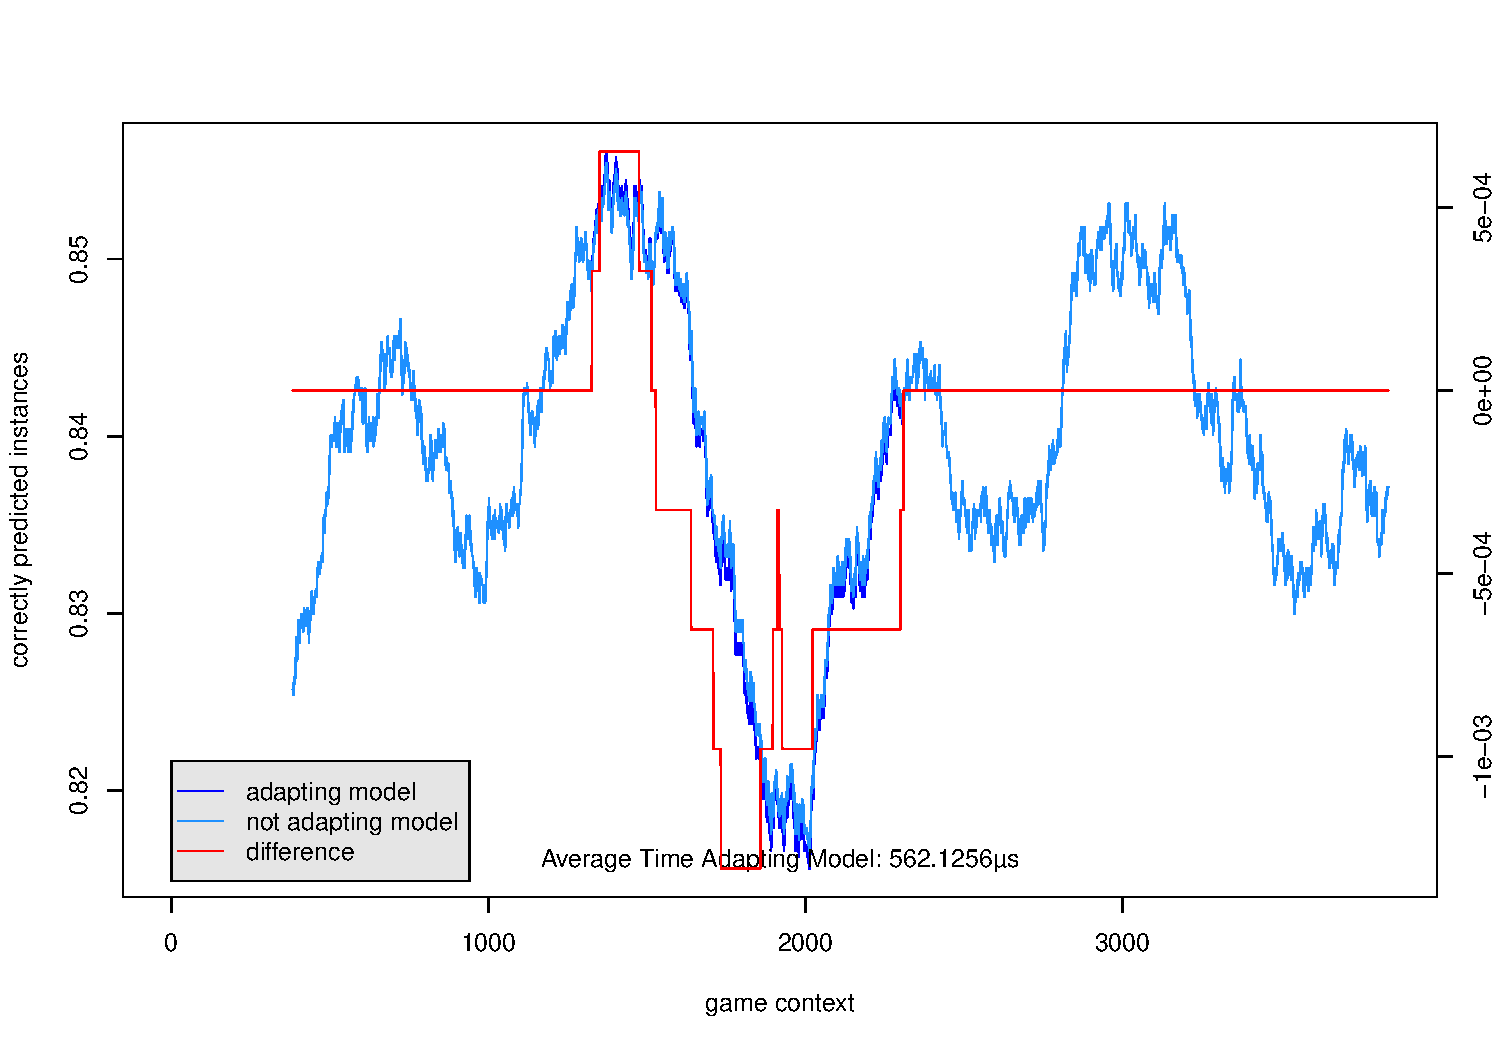
\includegraphics[scale=0.275]{section05-modelimpl/figures/HoeffdingTree-BluffBot4-action-correctly}
}


\caption{Action Prediction: Hoeffding Tree}
\label{fig:HoeffdingTree-action}
\end{figure}

\newpage
\subsection{Performance in Hand Prediction: Naive Bayes}
\begin{figure}[h!]
\centering

\subfigure[Model of HyperboreanNL-Eqm: Quadratic Loss]{
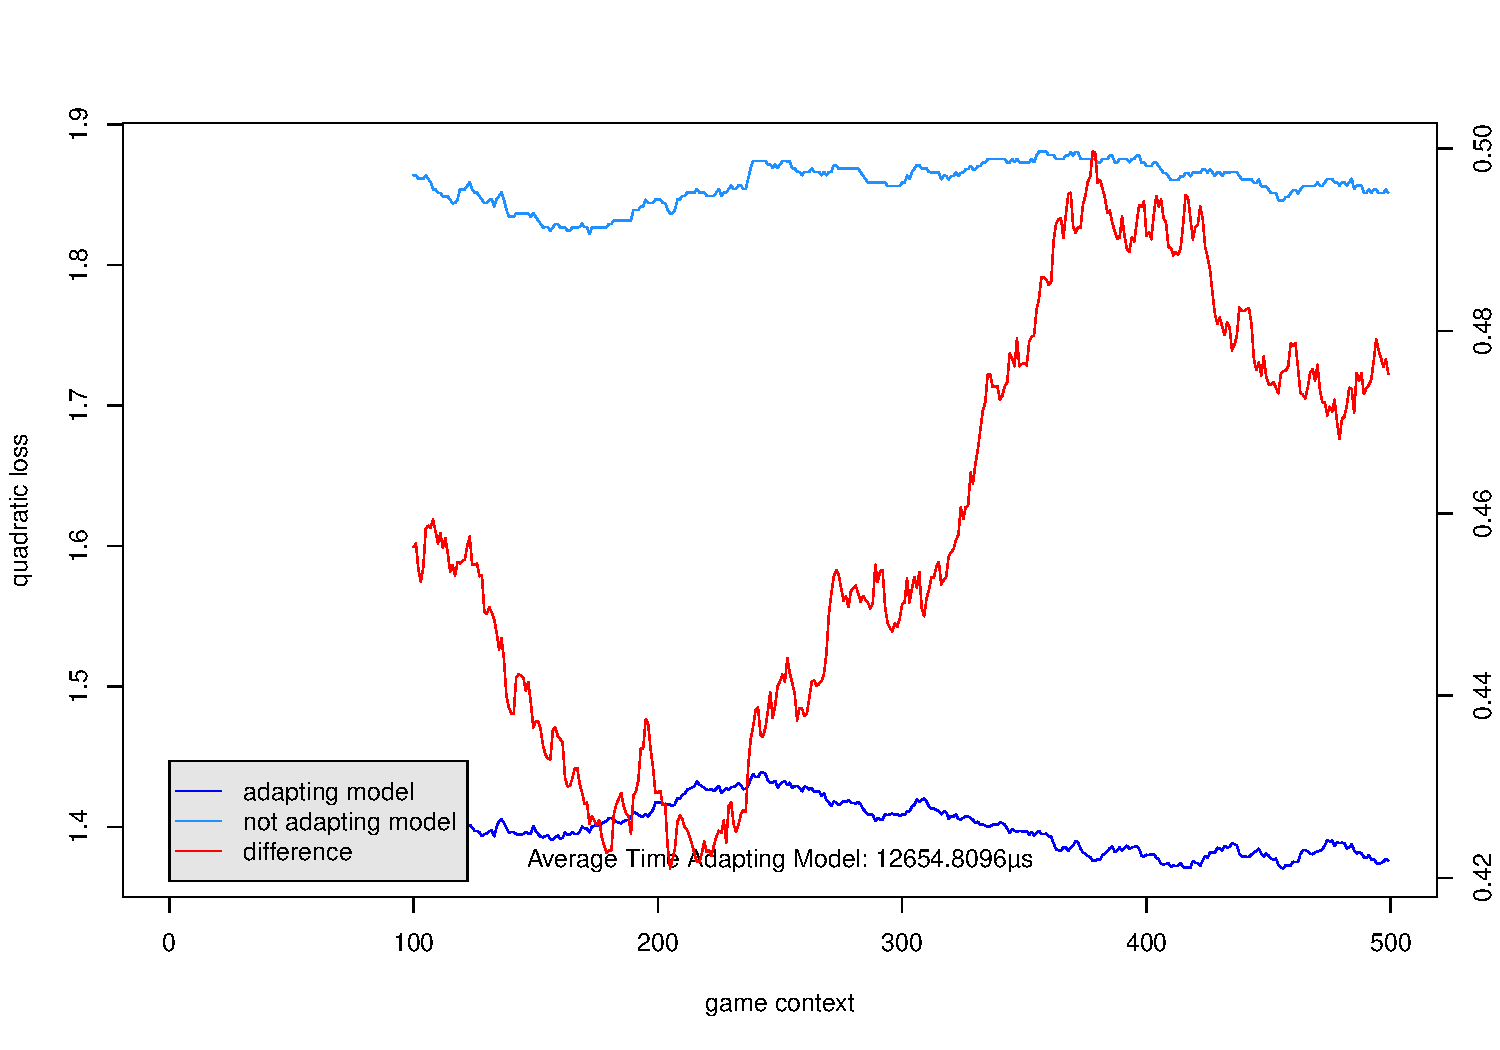
\includegraphics[scale=0.275]{section05-modelimpl/figures/MOANaiveBayes-HyperboreanNL-Eqm-hand-quadratic}
}
\subfigure[Model of HyperboreanNL-Eqm: Correctly Predicted]{
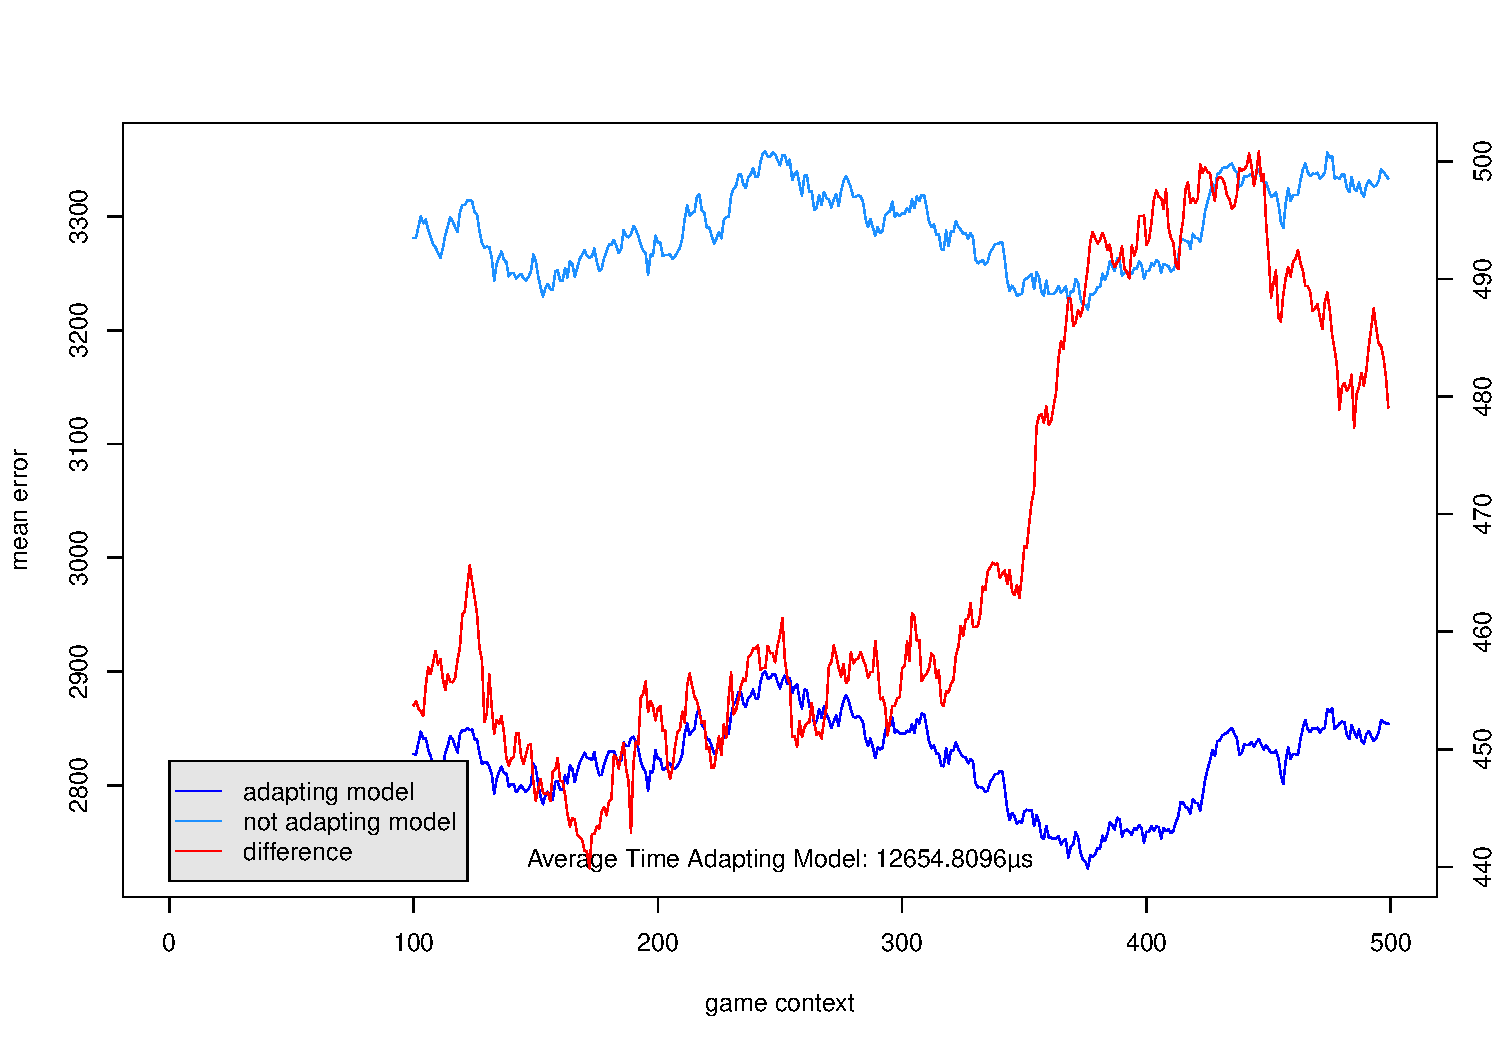
\includegraphics[scale=0.275]{section05-modelimpl/figures/MOANaiveBayes-HyperboreanNL-Eqm-hand-meansquared}
}

\subfigure[Model of HyperboreanNL-BR: Quadratic Loss]{
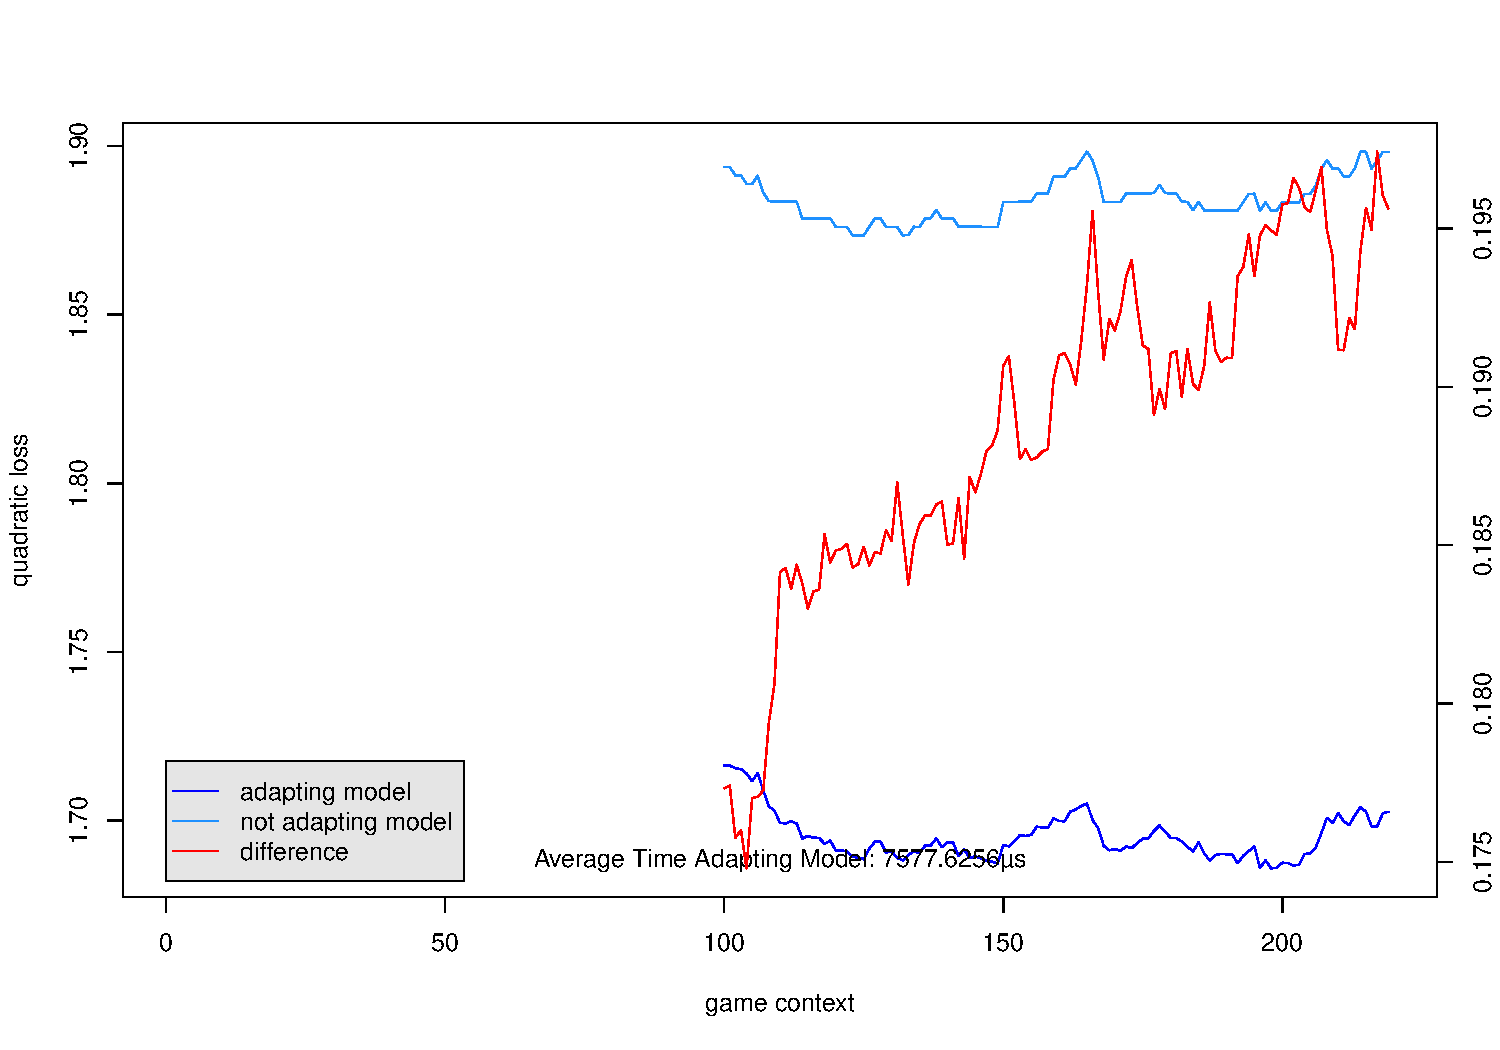
\includegraphics[scale=0.275]{section05-modelimpl/figures/MOANaiveBayes-HyperboreanNL-BR-hand-quadratic}
}
\subfigure[Model of HyperboreanNL-BR: Correctly Predicted]{
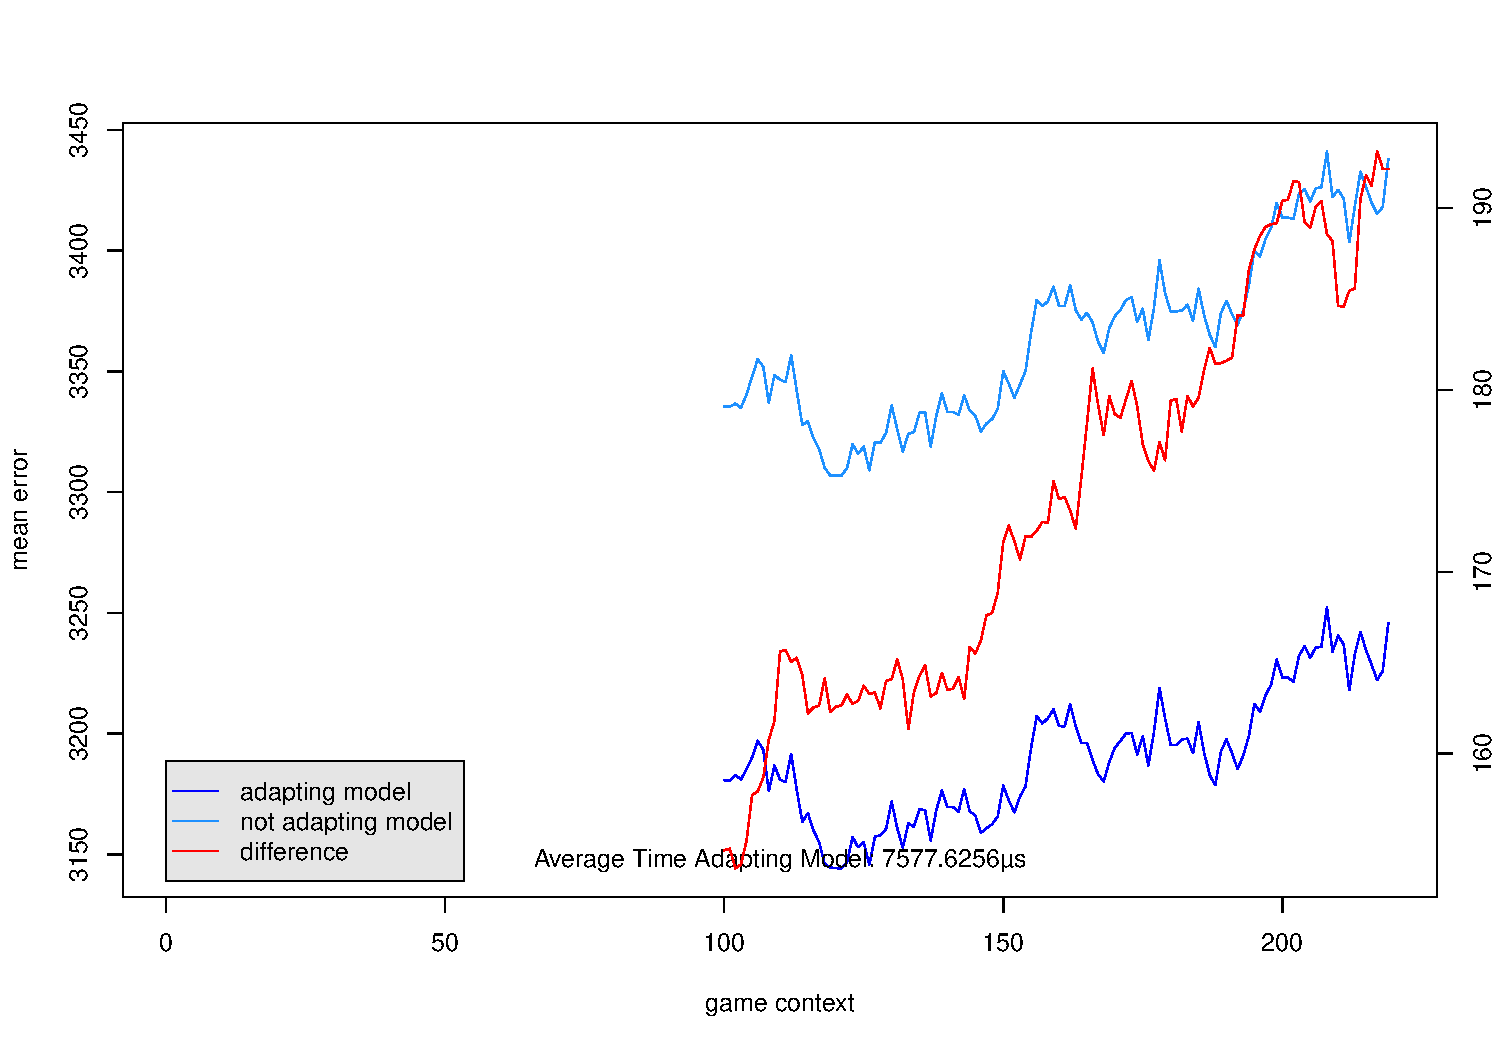
\includegraphics[scale=0.275]{section05-modelimpl/figures/MOANaiveBayes-HyperboreanNL-BR-hand-meansquared}
}

\subfigure[Model of BluffBot4: Quadratic Loss]{
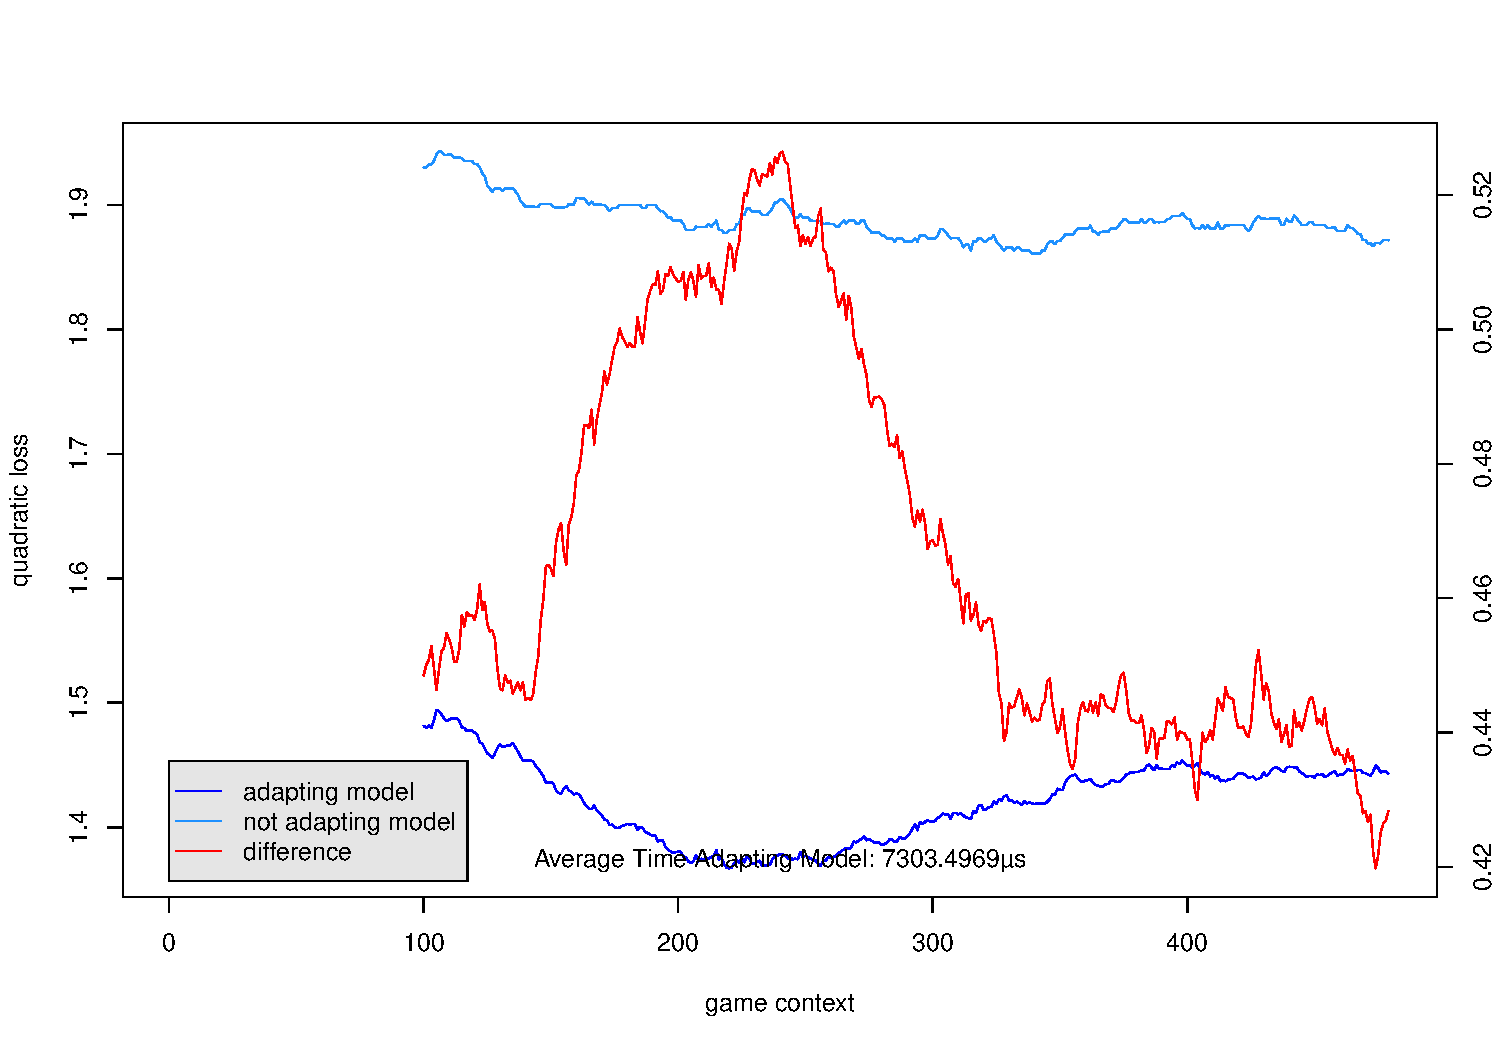
\includegraphics[scale=0.275]{section05-modelimpl/figures/MOANaiveBayes-BluffBot4-hand-quadratic}
}
\subfigure[Model of BluffBot4: Correctly Predicted]{
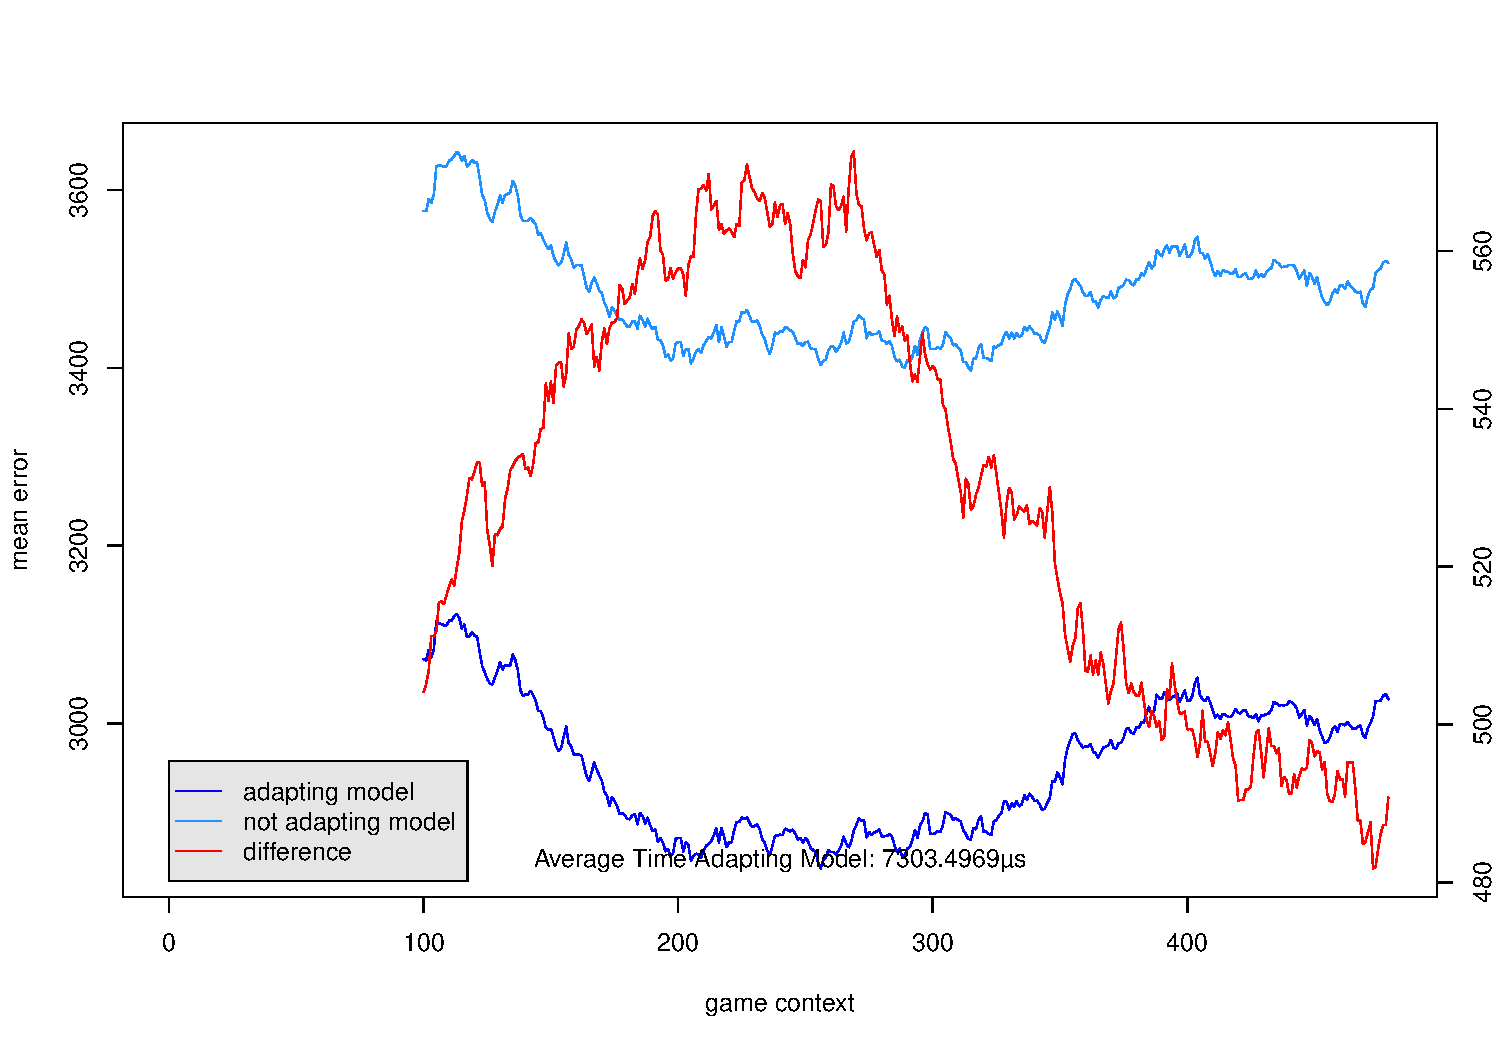
\includegraphics[scale=0.275]{section05-modelimpl/figures/MOANaiveBayes-BluffBot4-hand-meansquared}
}

\caption{Hand Prediction: Naive Bayes}
\label{fig:MOANaiveBayes-hand}
\end{figure}




\newpage
\subsection{Performance in Hand Prediction: Online Backpropagation}
\begin{figure}[h!]
\centering

\subfigure[Model of HyperboreanNL-Eqm: Quadratic Loss]{
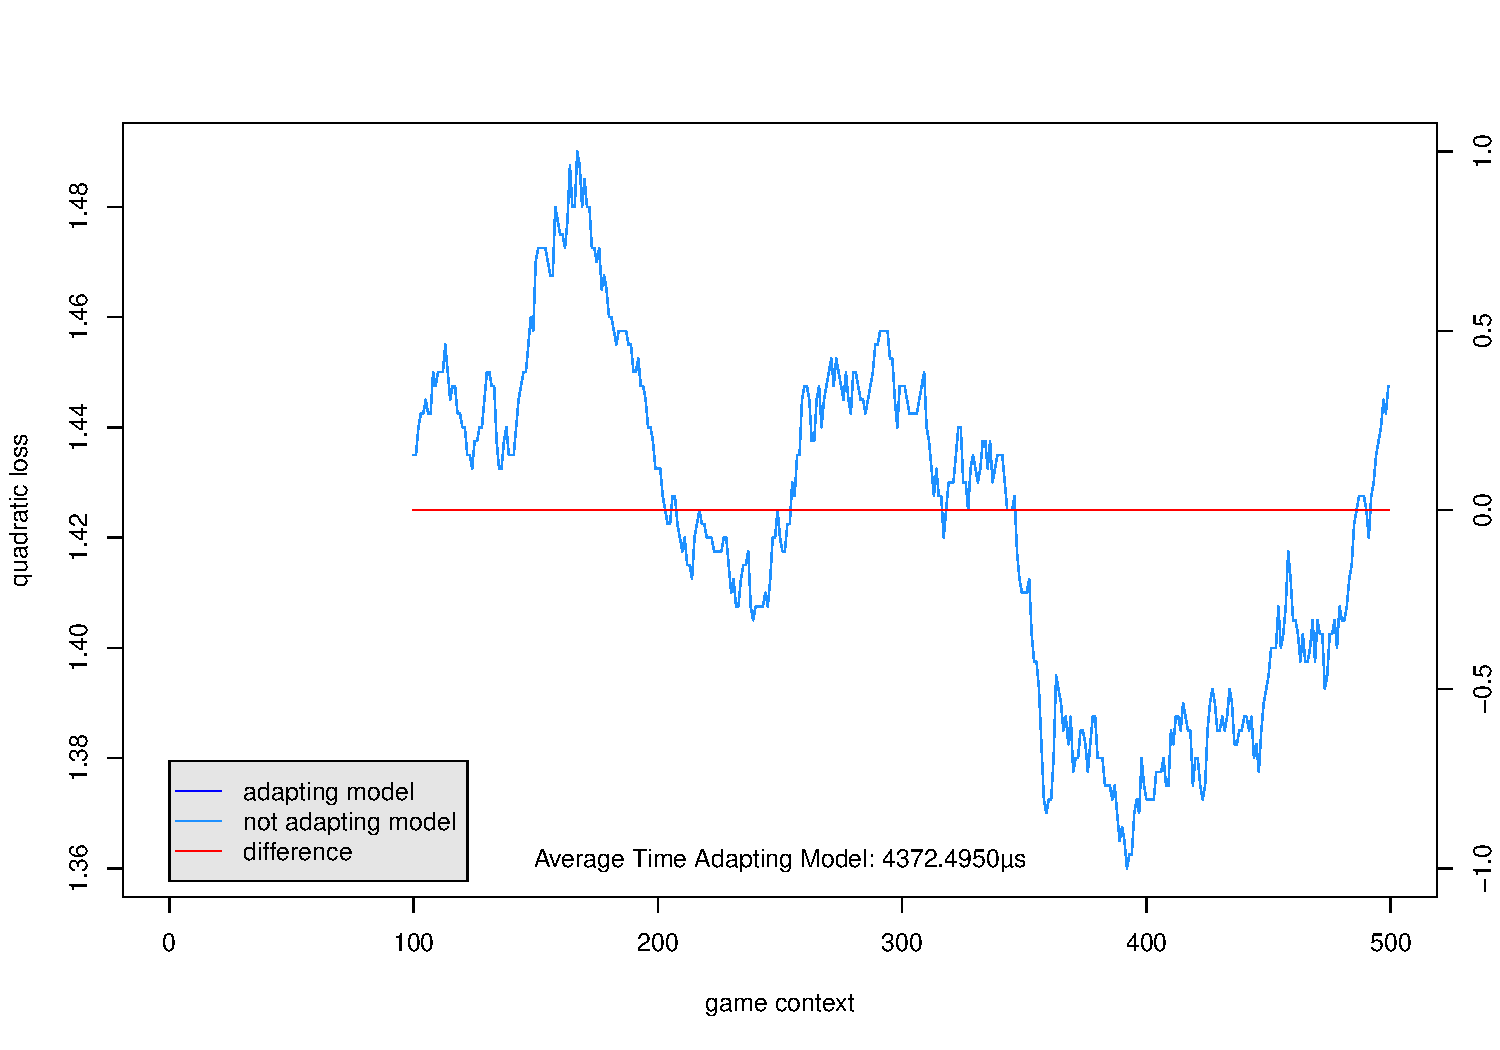
\includegraphics[scale=0.275]{section05-modelimpl/figures/OnlineBackpropagation-HyperboreanNL-Eqm-hand-quadratic}
}
\subfigure[Model of HyperboreanNL-Eqm: Mean Error]{
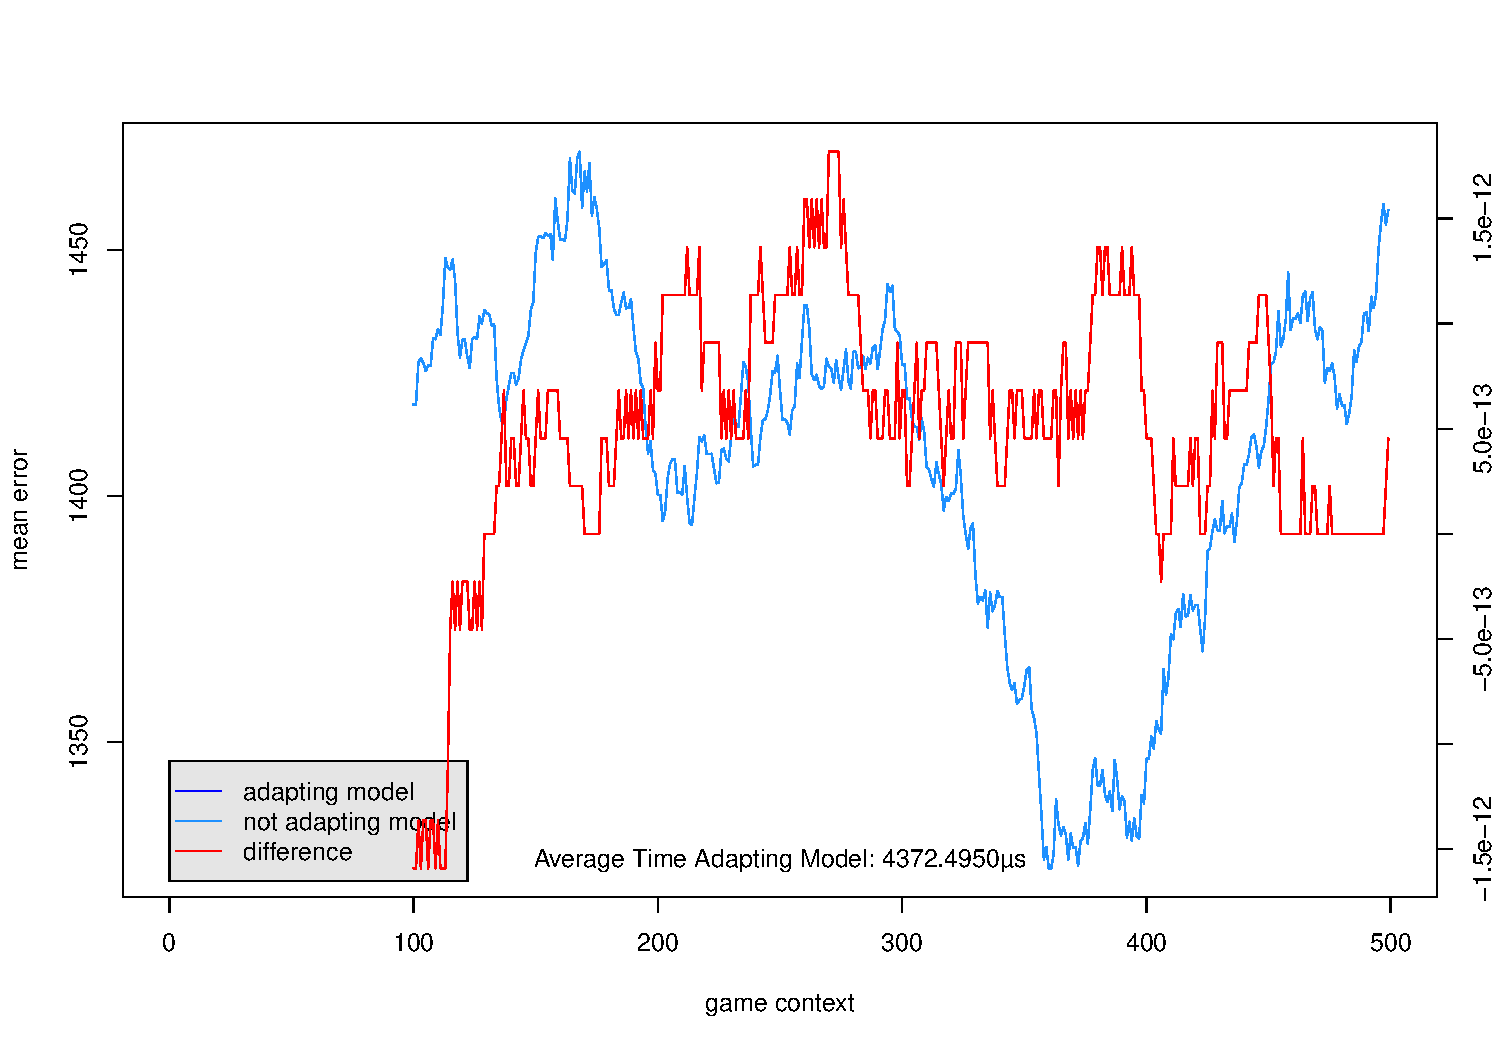
\includegraphics[scale=0.275]{section05-modelimpl/figures/OnlineBackpropagation-HyperboreanNL-Eqm-hand-meansquared}
}

\subfigure[Model of HyperboreanNL-BR: Quadratic Loss]{
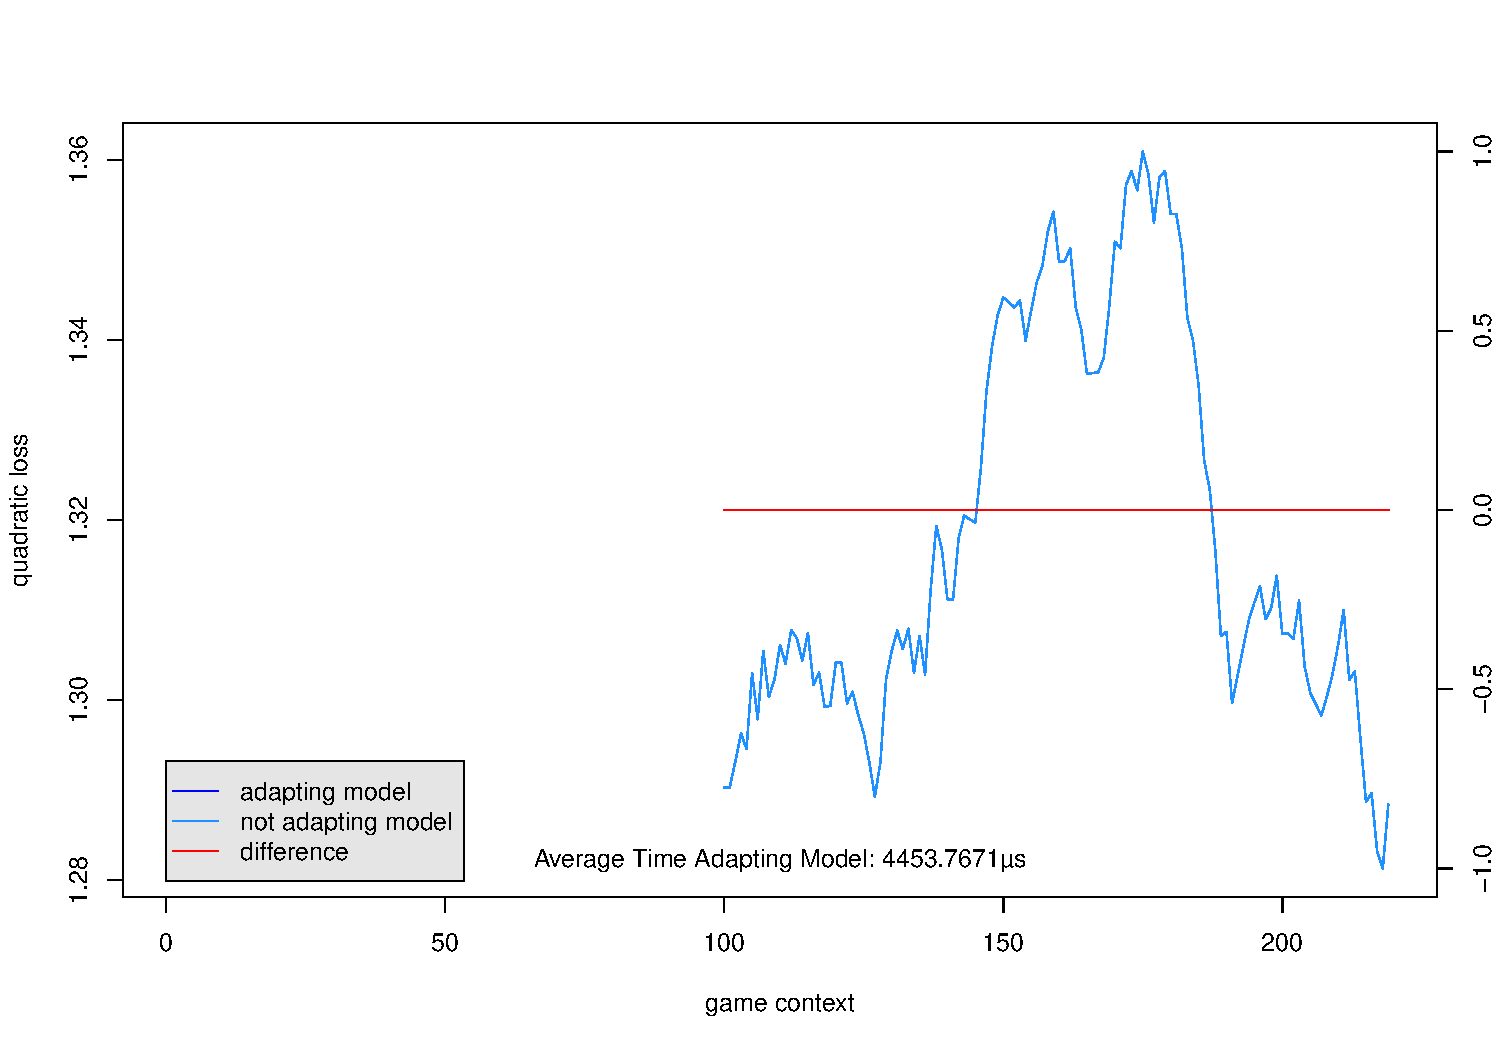
\includegraphics[scale=0.275]{section05-modelimpl/figures/OnlineBackpropagation-HyperboreanNL-BR-hand-quadratic}
}
\subfigure[Model of HyperboreanNL-BR: Mean Error]{
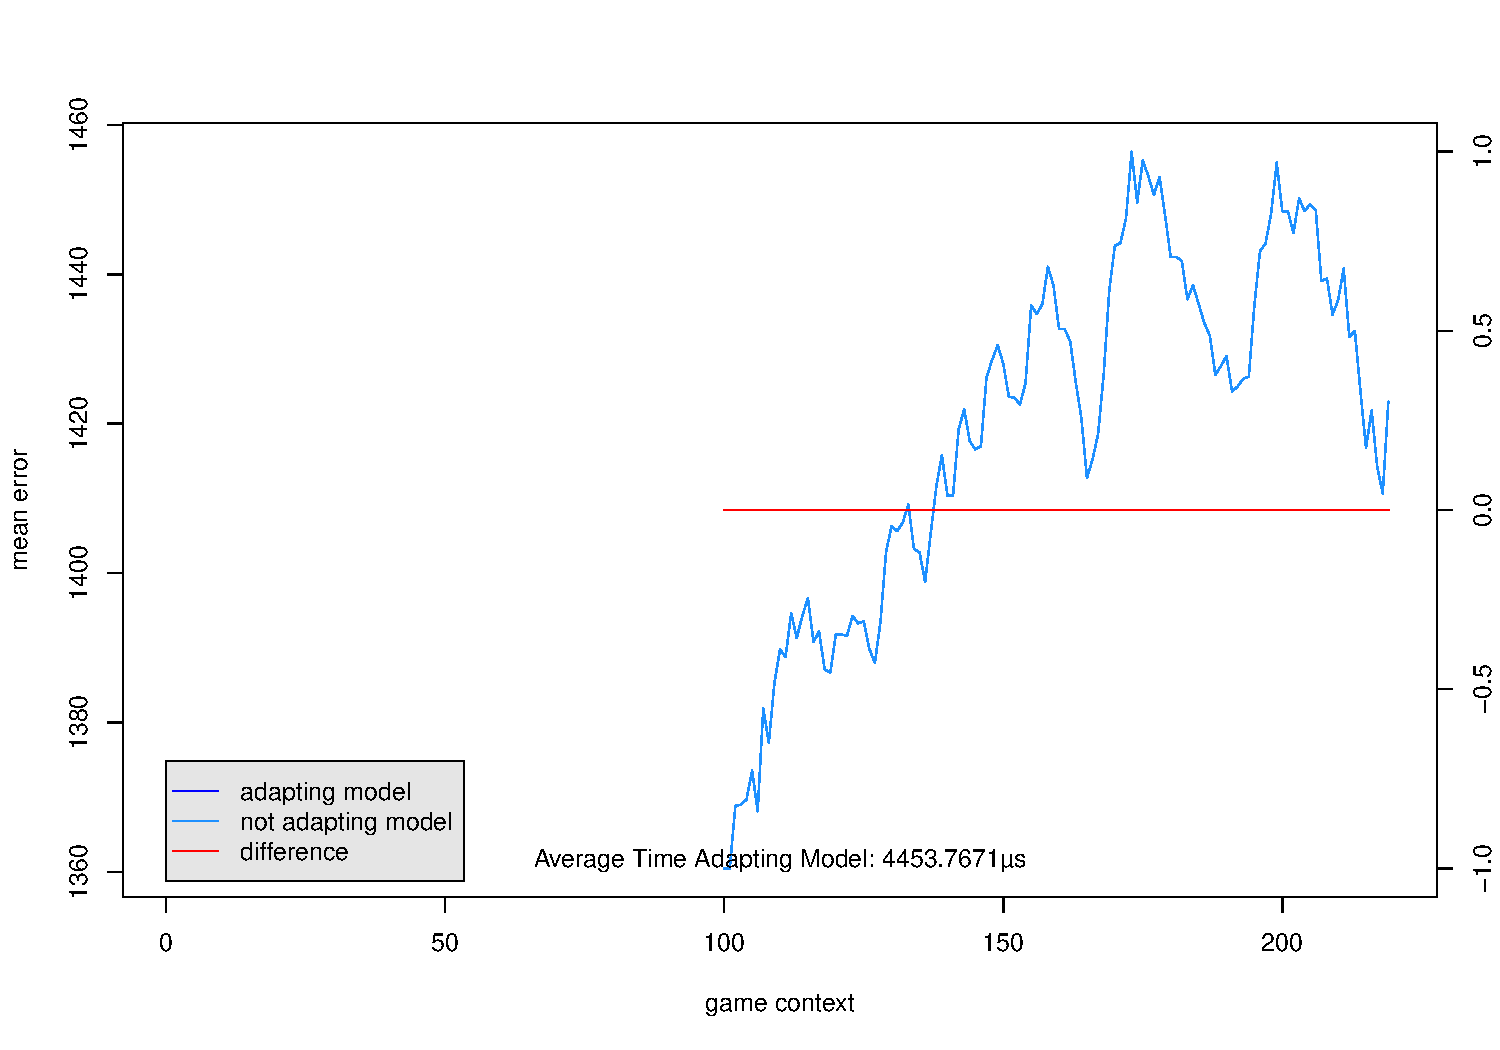
\includegraphics[scale=0.275]{section05-modelimpl/figures/OnlineBackpropagation-HyperboreanNL-BR-hand-meansquared}
}

\subfigure[Model of BluffBot4: Quadratic Loss]{
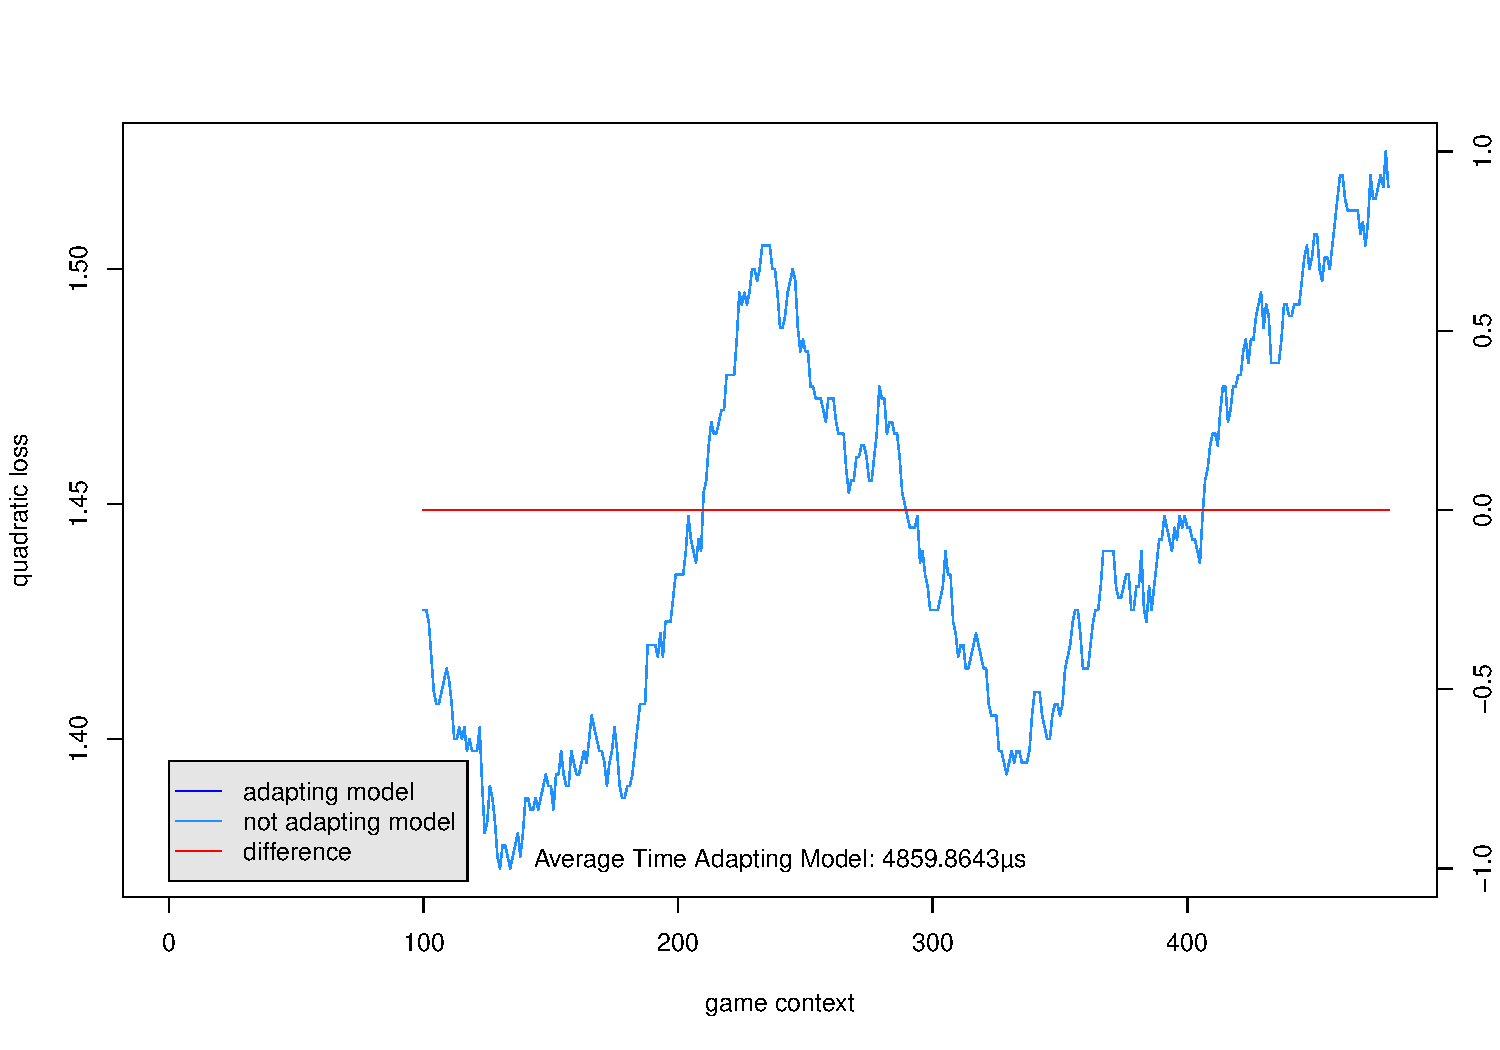
\includegraphics[scale=0.275]{section05-modelimpl/figures/OnlineBackpropagation-BluffBot4-hand-quadratic}
}
\subfigure[Model of BluffBot4: Mean Error]{
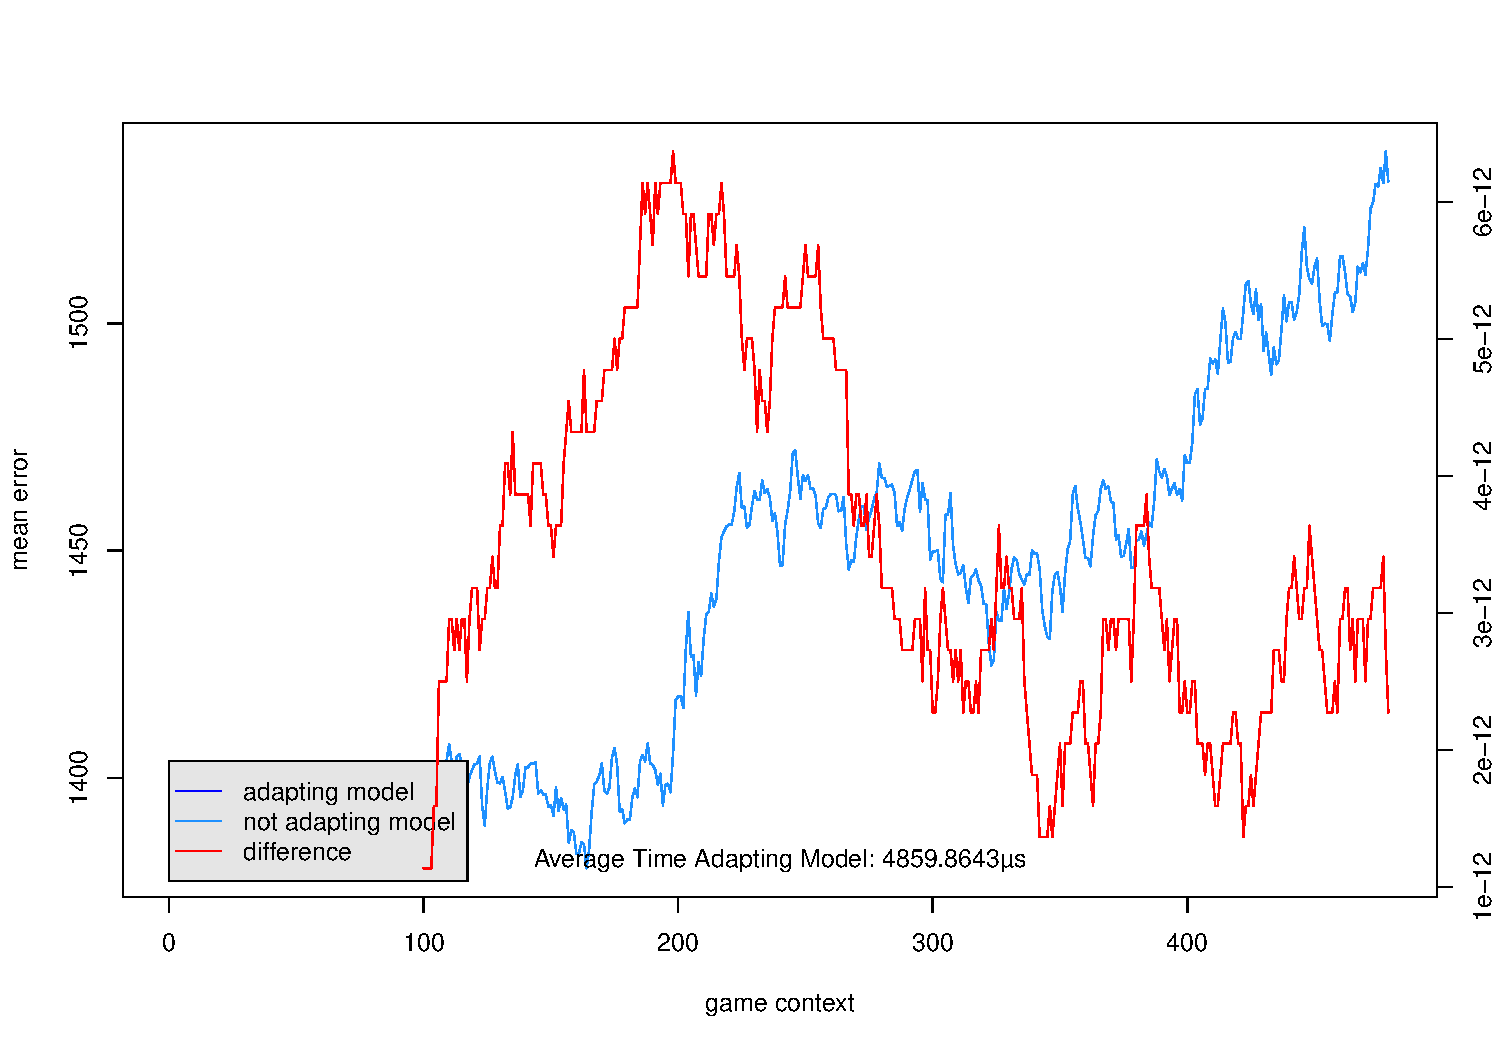
\includegraphics[scale=0.275]{section05-modelimpl/figures/OnlineBackpropagation-BluffBot4-hand-meansquared}
}

\caption{Hand Prediction: Online Backpropagation}
\label{fig:OnlineBackpropagation-hand}
\end{figure}


\newpage
\subsection{Performance in Hand Prediction: Hoeffding Tree}
\begin{figure}[h!]
\centering

\subfigure[Model of HyperboreanNL-Eqm: Quadratic Loss]{
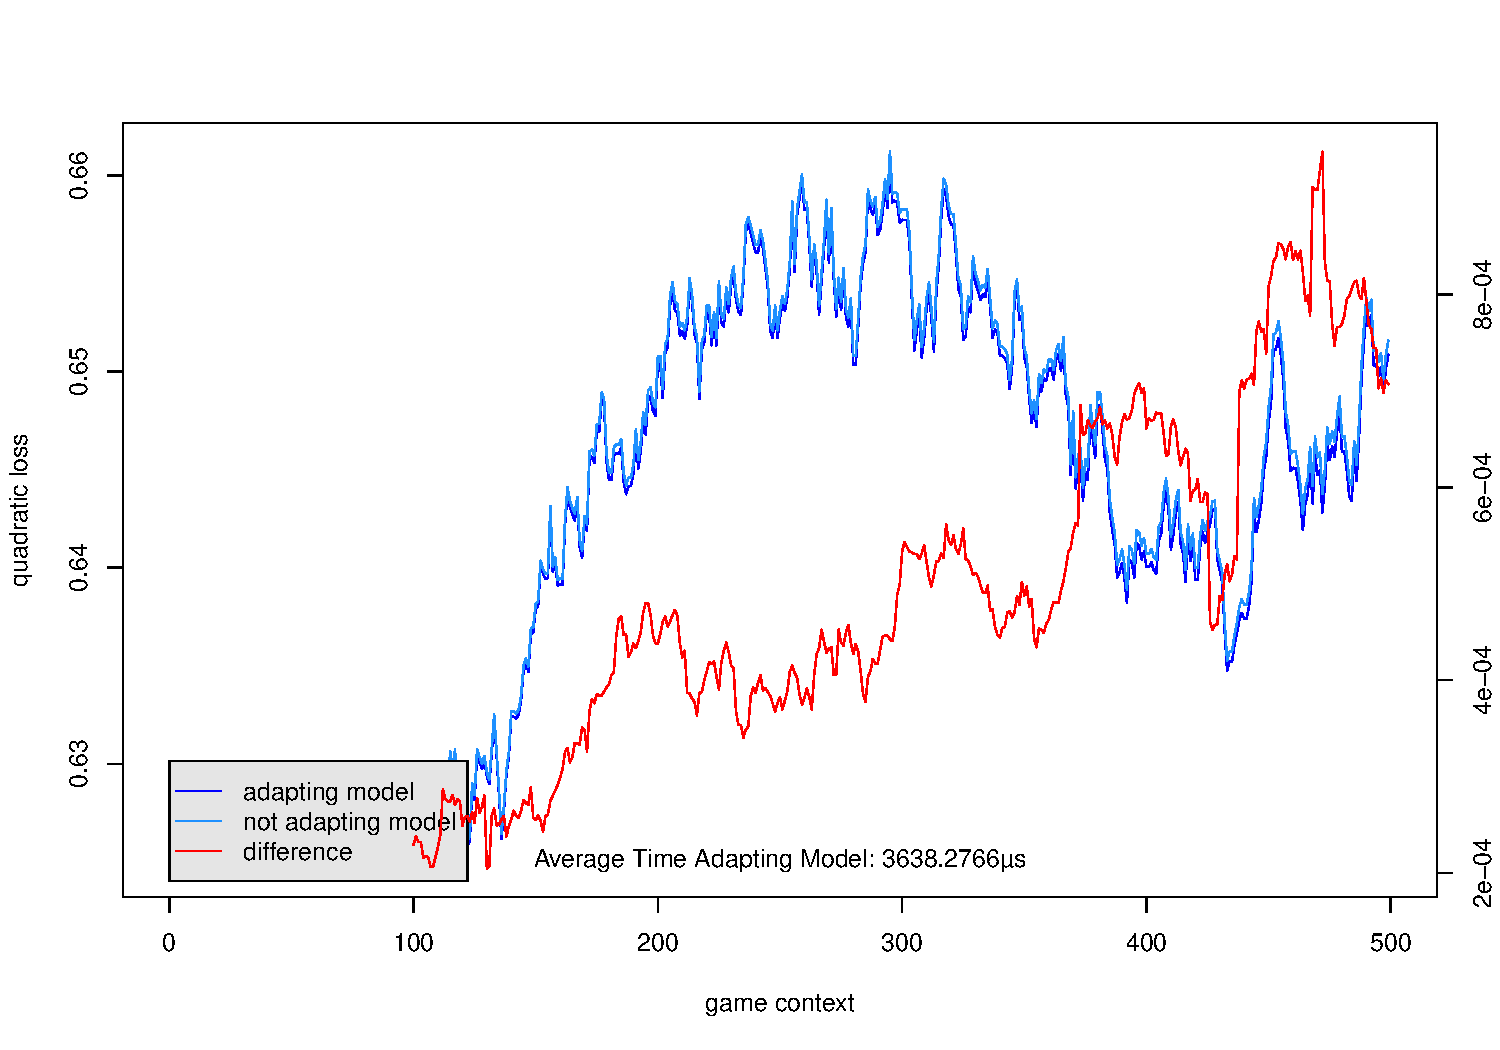
\includegraphics[scale=0.275]{section05-modelimpl/figures/HoeffdingTree-HyperboreanNL-Eqm-hand-quadratic}
}
\subfigure[Model of HyperboreanNL-Eqm: Mean Error]{
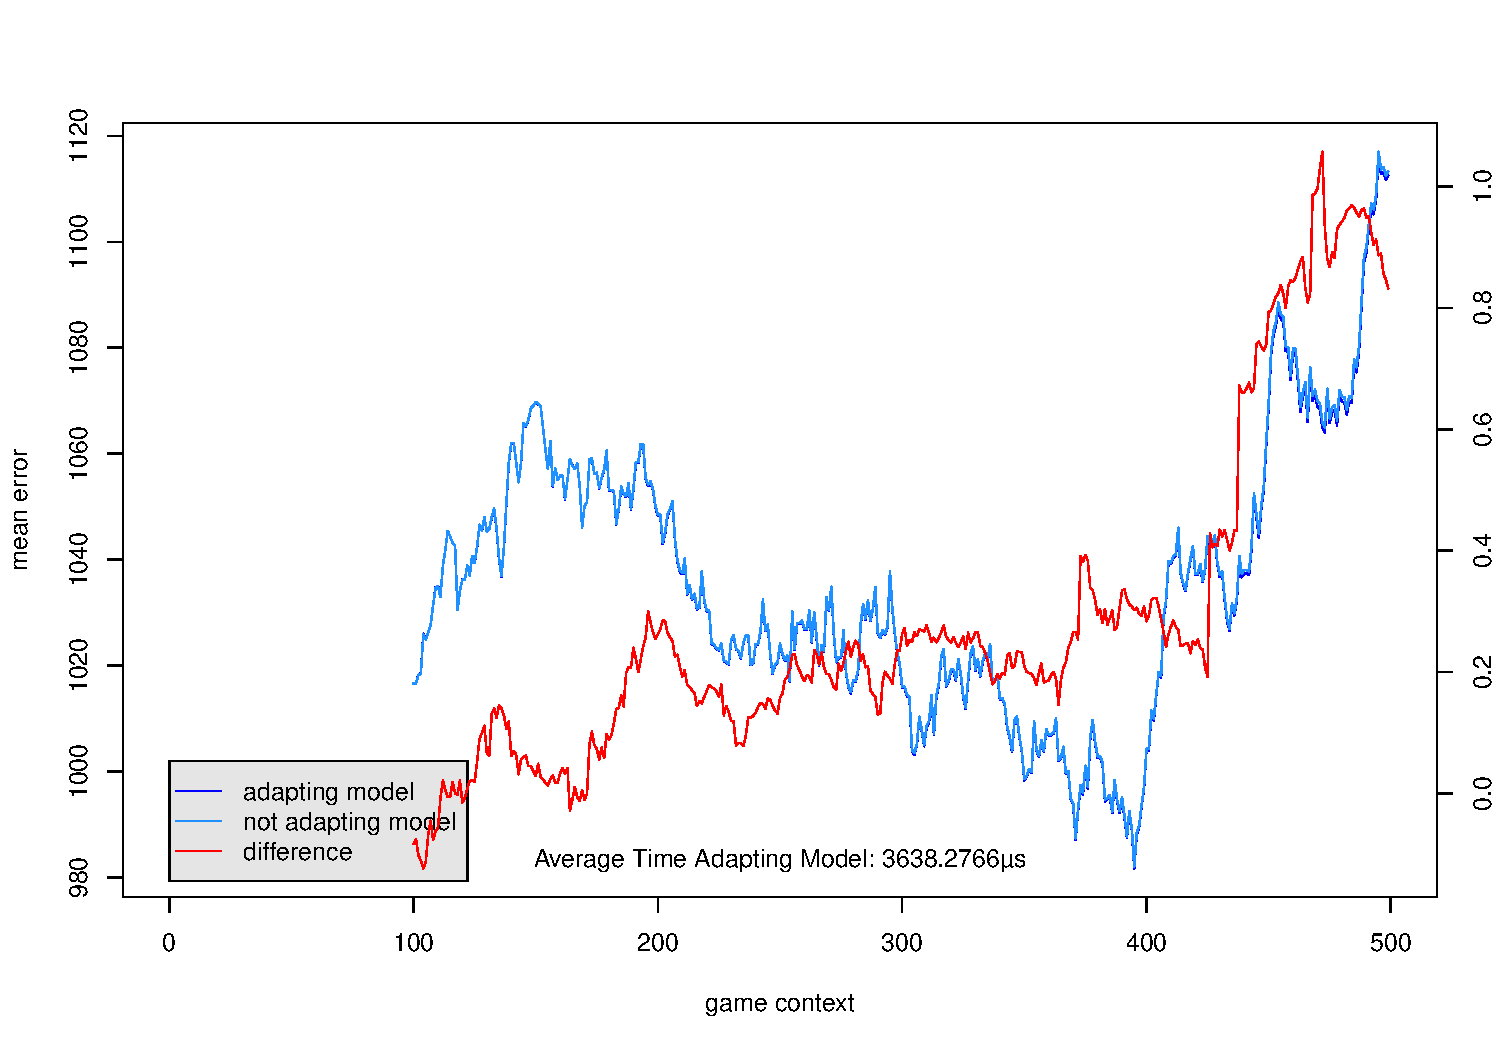
\includegraphics[scale=0.275]{section05-modelimpl/figures/HoeffdingTree-HyperboreanNL-Eqm-hand-meansquared}
}

\subfigure[Model of HyperboreanNL-BR: Quadratic Loss]{
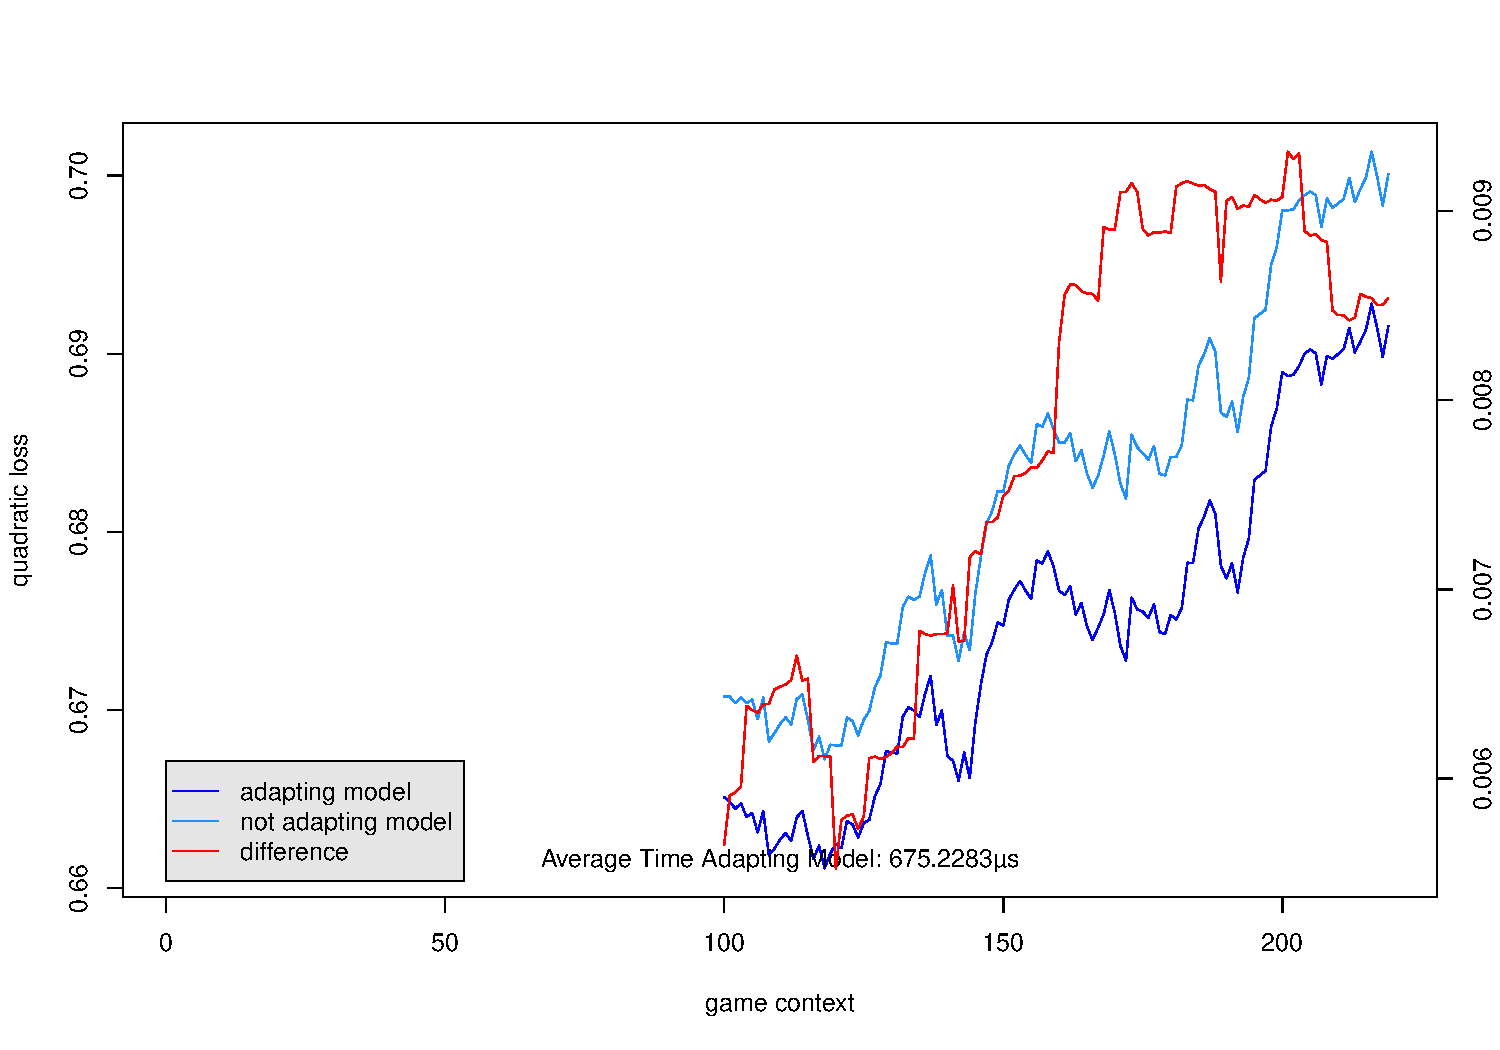
\includegraphics[scale=0.275]{section05-modelimpl/figures/HoeffdingTree-HyperboreanNL-BR-hand-quadratic}
}
\subfigure[Model of HyperboreanNL-BR: Mean Error]{
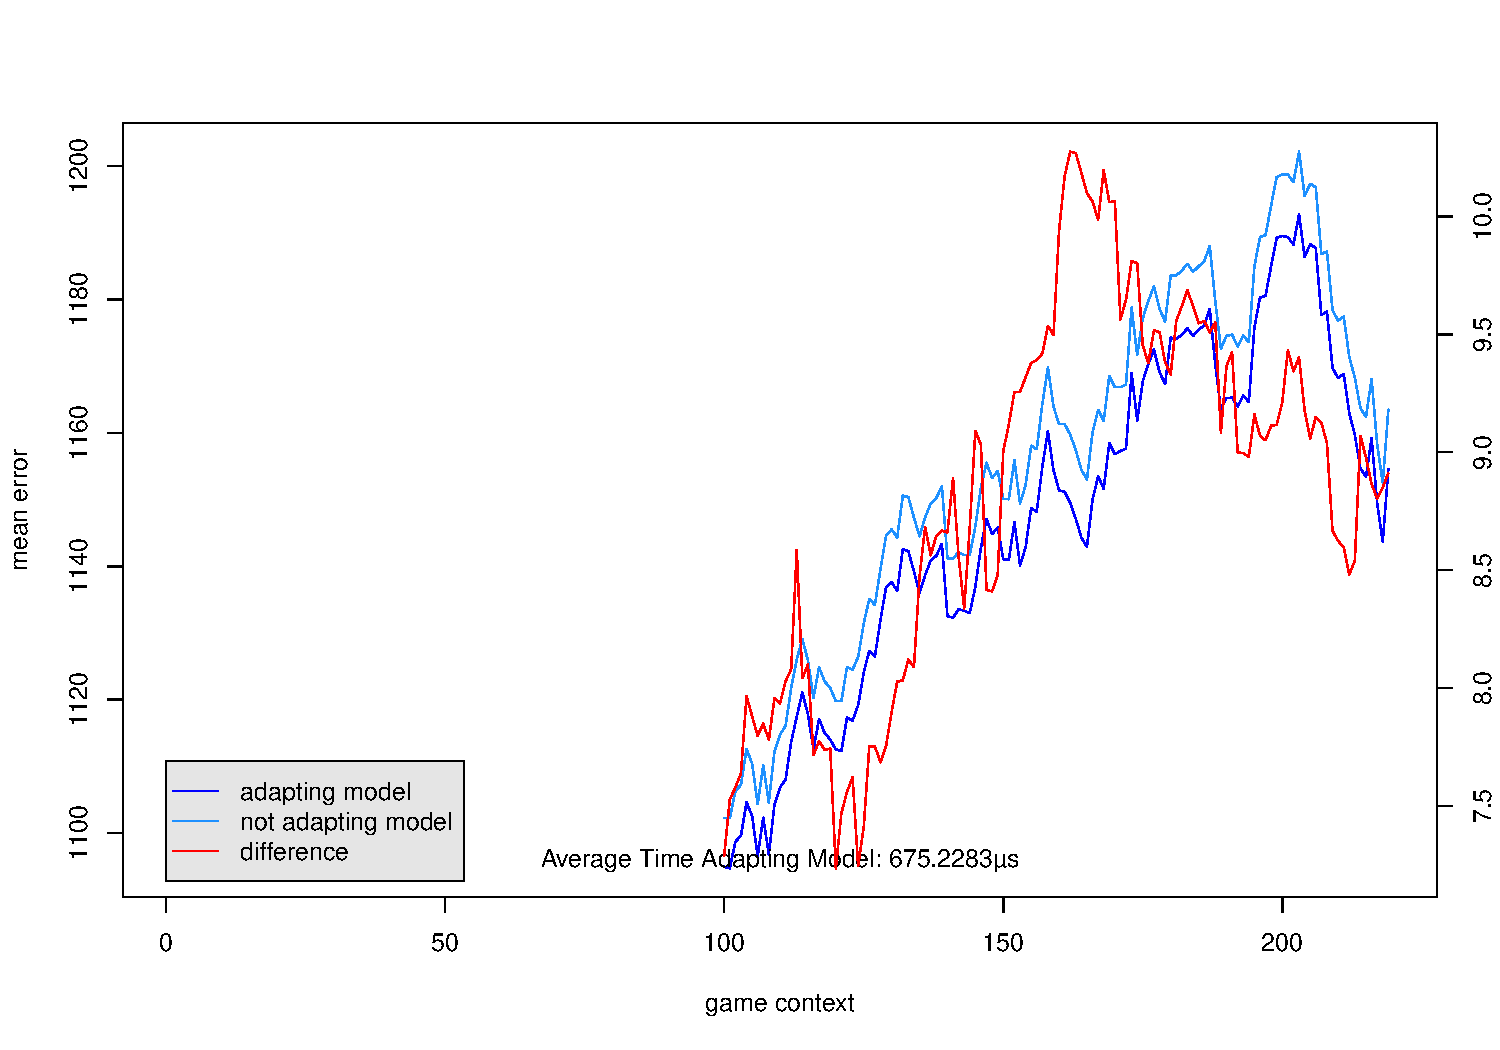
\includegraphics[scale=0.275]{section05-modelimpl/figures/HoeffdingTree-HyperboreanNL-BR-hand-meansquared}
}

\subfigure[Model of BluffBot4: Quadratic Loss]{
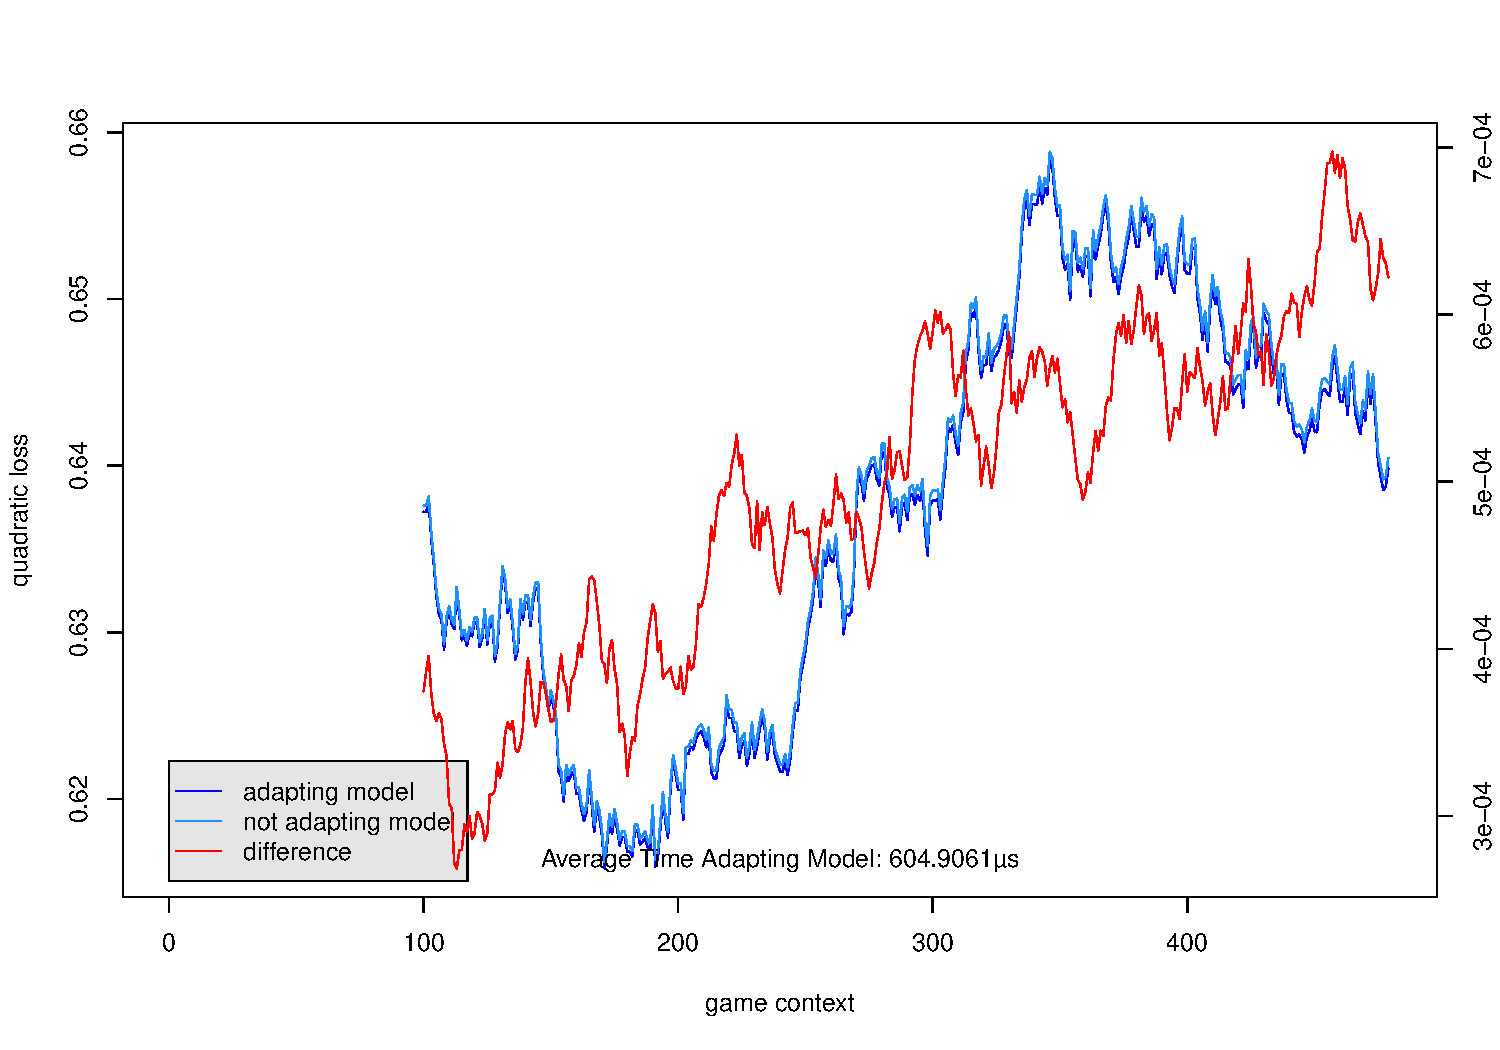
\includegraphics[scale=0.275]{section05-modelimpl/figures/HoeffdingTree-BluffBot4-hand-quadratic}
}
\subfigure[Model of BluffBot4: Mean Error]{
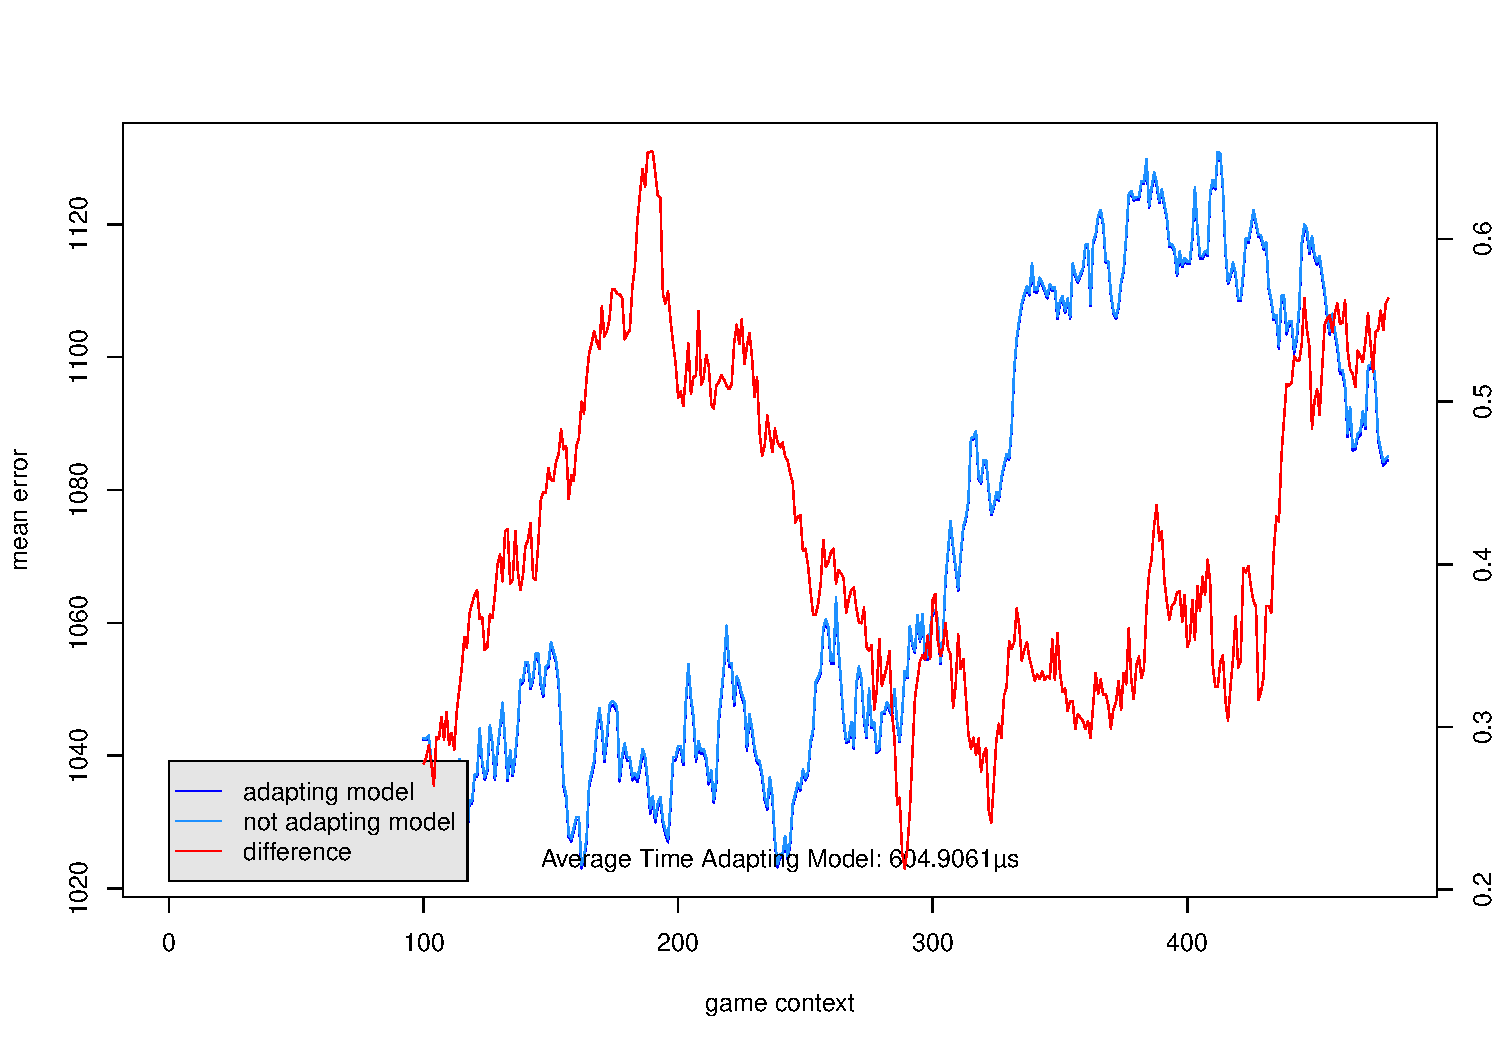
\includegraphics[scale=0.275]{section05-modelimpl/figures/HoeffdingTree-BluffBot4-hand-meansquared}
}


\caption{Hand Prediction: Hoeffding Tree}
\label{fig:HoeffdingTree-hand}
\end{figure}



\newpage

\subsection{Conclusion}
 
\subsubsection{Naive Bayes}
Naive bayes was added to the benchmark as a simple comparison measure. While showing the strongest adaption, naive bayes generally didn't fare very well on both predictions. This couldn't be compensated with the very strong increase during a match.

Additionally, the classification speed alone was by far the slowest, so slow that it could not be used in a live game of poker anyway.

\subsubsection{Online Backpropagation}
Unfortunately, the computational cost to build an opponent model was too great to build the prior with the same number of observations as the other two algorithms, which used a dataset of millions of observations. For the online backpropagation, I restricted this to a few tens of thousands. 

Probably for this reason, classifications made with the online backpropagation, was not much stronger then with naive bayes - some times even weaker. Unfortunately as \cite{Davidson2002} mentioned, the much more important distribution accuracy measured with the quadratic loss was extremely weak.

Additionally, because only few samples were available at each update step (hand prediciton was updated with datasets of 5 observations, action prediction after 50 observations), the online trainer couldn't improve the predictions - resulting in a horizontal red line, showing that the trainer had to reset the network after each update. In other cases, the prediction quality even declined.

While being faster than naive bayes, online backpropagation was still so slow, it would only be usable with much faster hardware than currently available to me.

\subsubsection{Hoeffding Tree}
Hoeffding generally showed a good prediction and distribution accuracy. It didn't adapt as fast as naive bayes, but the stronger performance of the prior made easily up for this disadvantage.

Little surprising, since designed for fast prediction, the Hoeffding tree algorithm was able to classify the instances extremely fast - usually in just a fraction of a milisecond.


\chapter{Implementation}
\label{chap:implementation} 

When implementing the Miximax algorithm presented in chapter \ref{c:game-tree-search}, one quickly realizes that poker unfortunately is too complex to be completely represented in a search tree.

The standard rules of Limit Hold'em allow for a maximum of four bets per player per round. Thus, in 2-player Limit poker there are 19 possible betting sequences, of which two do not occur in practice (e.g. check-fold). Of the remaining 17 sequences, 8 end in a fold (leading to a terminal node in the game tree), and 9 end in a call (carrying forward \cite{Billings2006}. This gets repeated in each stage of the game. In No-Limit Texas Hold'em, such calculations aren't possible, as theres no maximum of bets, and a unlimited number of bets per stage. But it is obvious that compared to Limit Hold'em, No-Limit results in a much more complex tree than Limit Hold'em, even with abstracted actions and a limited amount of bets.


\begin{table}[!ht]
  \begin{tabular}{ l|l}
\textbf{Decision Point Where Search is Invoked}�& \textbf{\# of Leaves in Search Tree}�\\
 \hline
 start of game before preflop cards are dealt & $\approx$ 697 trillion\\
after preflop cards are dealt & $\approx$ 525 billion\\
before flop cards are dealt & $\approx$ 58.5 billion\\
after flop cards are dealt & $\approx$ 2.98 million\\
before turn card is dealt & 331'162\\
after turn card is dealt & 7'046\\
before river card is dealt & 782\\
after river card is dealt & 17\\
 \end{tabular}
 
\caption{Number of Leaves in 2-player Texas Hold'em Search Tree when First to Act (calculated by \cite{Schauenberg2006})}


\label{fig:leaves-count}
\end{table}

\begin{table}[!ht]
  \begin{tabular}{ l|l}
\textbf{Decision Point Where Search is Invoked}�& \textbf{\# of Leaves in Search Tree}�\\
 \hline
after preflop cards are dealt and check & $\approx$ 292 billion\\
after flop cards are dealt and check & $\approx$ 1.656 million\\
after turn card is dealt and check & 3'914\\
after river card is dealt and check & 9\\
 \end{tabular}
 
\caption{Number of Leaves in 2-player Texas Hold'em Search Tree when Second to act Following a Check (calculated by \cite{Schauenberg2006})}


\label{fig:leaves-count2}
\end{table}

In chapter \ref{c:game-tree-search}, I always assumed to build a game-tree of all possible actions, both for the player as well as for the opponent. Unfortunately, this is not feasible when trying to actually implement such an algorithm. Poker, even limit-poker is far to complex to completely model. Table \ref{fig:leaves-count} shows the number of leave nodes different game trees at certain stages in the game, as calculated by \cite{Schauenberg2006} for Limit Texas Hold'em.

When facing implementation two things have to be taking into consideration. First: all these nodes have to be initiated and traversed, as well as all opponent nodes being subject to a (more or less) sophisticated opponent prediction model. Second: For limit poker, the number of actions is always limited to 3 (fold/check/bet or fold/call/raise), with folding obviously being dominated when checking is possible. In no-limit, the number of actions is dependent on a players stack size (in relation to the blinds), but virtually infinite. These leads to two practical search challenges:

\begin{itemize}
	\item The number of possible actions has to be shrunk to a reasonable amount, to keep the branch factor at least under control.
	\item Even after limiting the number of possible action, at least on the preflop and flop-stage, the game tree cannot be fully traversed. 
\end{itemize}

\section{The Action Model}
\label{s:ActionAbstraction} 

In limit Texas Hold'em, the players only ever have at most three possible actions available to them (fold, call, or raise). This controllable branching factor, allows for a full representation of the game - at least in situation where simulations can be reused - like in equilibrium calculations done offline.

In No-Limit Texas Hold'em, on the other hand, the number of actions available to the players can be huge. For example, given a blind-level of 1\$-2\$ the small blind makes his first action, he can fold, call, or raise to any (integral) amount between 1 and 198, for a total of 199 possible actions (assuming stacks limited to 100 big blind, and if the bets were not limited to be integral amounts then the branching factor would actually be infinite). And this branching factor would actually occur at every decision node in the game tree.

\cite{Gilpin2008} estimates, with bets limited to integers, the size of the not abstracted game tree of no-limit heads-up Texas Hold'em to be approximately $10^71$ nodes.

Thanks to game theoretic realities, only a limited amount of actions make sense in no limit poker. Both bets too small, as well as to big (relative to the pot size) are usually a bad idea \cite{Sklansky1999} \cite{Chen2006} \cite{Sklansky2006}. When facing such a bet, the opponent has favorable pot odds (the relation of the amount an opponent has to call to the amount already in the pot) to make a call. Whatever we think he holds, or he thinks we hold, the amount to pay to see the next card is justifiable with simple statistics.

These poker theoretic fundamentals allow us to limit the branching factor of  the tree significantly by discretizing betting amounts into a very limited number of abstracted actions. My abstracted actions include the three bet amounts used  by \cite{Andersson2006}. This abstraction of the real game, now finally allows us to see predicting the opponent actions as as classification problem. We can simply classify the (abstracted) game situation represented by a opponent node into action classes. These Action Classes, include the following actions:

\begin{itemize}
	\item \textit{Fold:} laying down cards when the opponent called.  No abstraction is required here, since there's only one way to fold (a player can't fold only part of a wager). 
	\item \textit{Check:} not waging any bet, passing the action on to the opponent. This does not need to be abstracted either.
	\item \textit{Call:} paying the opponents wager. Also no abstraction involved, as there is only one legal way to call a bet.
	\item \textit{Bet/Raise:} while technically two different actions, there is only one single action that is legal. The betting amount though is only governed by the amount of the big blind and the stack of the opponent - meaning that the betting amount must be abstracted, to lower the theoretically infinite branching factor.
\end{itemize}

To abstract the betting amounts, the game tree only models oppont and player actions in the following amounts also used by \cite{Gilpin2008} and \cite{Andersson2006} and also regarded as roughly best-practice in poker literature (e.g. by \cite{Sklansky2006}, \cite{Harrington2004}):

\begin{itemize}
	\item \textit{Bets equal to half of the pot} are good value bets, as well as good bluffs. When a player has a strong hand, by placing a half-pot bet he is giving the opponent 3:1 odds. What that means is, that the opponent only needs a better hand in 25\% of the cases, making it an attractive call. On the other hand, they are also an interesting bluff: They only need to work one time in three in order for it to be a profitable play.
		\item \textit{Bets equal to the size of the current pot} are useful, when a player currently has a stronger hand than his opponent and the deck suggests his opponent might "draw out". By placing a pot bet, the player is taking away the odds that the opponent would need to rationally call the bet with almost any drawing hand, that is, a hand that is not good currently, but has the potential to improve with additional cards.  It is usually not necessary to bet more than this amount, and a higher bet would only put the cost higher in case the player is not holding the leading hand as expected.
		
		Pot bets are particularly useful pre-flop when the big blind, who will be out of position (i.e., acting first) in
later betting rounds, wishes to make it more expensive for the small blind to play a particular hand.
	\item \textit{Going all-in} usually is not a good idea. If the opponent makes the call, he most likely has a better hand, and if he does not make the call, there was usually put too much money on the line to take down a rather small pot. However, it is a commonly used move (often by beginners). In some situations, where the pot is relatively large relative to a players remaining chips, it's better to go all-in, then to be forced to call with the remaining chips. 
	
	Another good reason for including the all-in bet in the model is that it provides a level of robustness in the model. 
	\end{itemize}

Since these three amounts are only a crude estimation of all possible moves, \cite{Gilpin2008} also outlined some of the other possible amounts, and why they are not included in the abstraction:


\begin{itemize}
\item \textit{Small Bets} in relation to the pot are usually a bad move. When the opponent faces such a bet, he usually has terrific pot odds to call them. Since he only pays relatively little for a chance to win a larger pot, he can also play cards with a low chance of improving. Additionally, a small bet provides little gain if called. If the opponent calls because he believes to have a better hand, he probably would also have called a larger hand.
\item \textit{Large Bets} in relation to the pot, but not all-in usually drain a players stack fast. Once a player's quantity of remaining chips gets low in relation to the pot, he is in a situation known as pot-committed. When facing a subsequent bet of any size, the player will be facing great odds, because he can call with whatever he has left, even if that amount is drastically smaller than the pot.  In this sense, a rational player who is pot-committed is basically in the same situation as a player who went all-in already. Thus bets that lead to pot-committed situations are, in a sense, nearly redundant. 

For this reason, \cite{Gilpin2008} advocates to not allow bets that place a player or opponent in a pot-committed situation. To prevent this, I added an amount the player must have after adding another child to a decision node. If this condition can't be fulfilled, the action would not be added, and implicit be included in the all-in action, which will always be added. Since stacks in the test setting are synchronous, this also asserts that the opponent wont be  put in such a situation if he calls.
\end{itemize}


These three bets together with call, fold or check define the maximal number of children of any (player or
opponent) decision node. 

Other approaches also abstract the amount of actions a players and opponents can take during a betting round (stage). In Limit-Poker there each player is allowed to only bet 4 times each stage. Most literature (\cite{Billings2006b}, \cite{Schauenberg2006}, \cite{Johanson2007}) for limit bots only simulate 3 bets per stage. In No-Limit Poker, there's no-limit on how many bets players can make. Theoretically, they could each raising by the big blinds for dozens of times, until one of them is all-in. \cite{Gilpin2008} like his colleagues researching limit poker, also advocated a limit of 3 bets per stage. But in a footnote obviously added later on, he notices that in reality the abstracted betting model limits the amount of possible actions anyway, since the players are all-in after 3 or 5 bets.

I implemented such a limit, but later on disabled it, since I found out that it does not provide any significant limitations of the game tree for the same reasons as \cite{Gilpin2008} noted.

So, taking the above considerations all into account, the final betting model allows for the following actions (and therefore branches in the game tree):

\begin{enumerate}
	\item Both players always have the option of going all-in
	\item When no bets have been placed within a betting round, a player can either check, bet half the pot, bet the amount currently in the pot or go all-n.
	\item After a bet has been placed already in the current stage, a player can either fold, call, bet the pot or go all-in.
	\item If at any bet (all-in excluded) would commit more than half of a players stack, that bet would not be added to the game tree.
\end{enumerate}

With more incorporation of domain knowledge, this model could probably be refined further. Perhaps, against some opponents, one-third or two-third bets might be better than always assuming a bet of half the size of the pot.


\subsection{Reverse Mapping of Actions}
\label{s:ActionAbstraction2} 

Obviously, in the real game an opponent (or an observed player when building the prior of the opponent model) does not follow these abstractions of the action model. These actions still have to be mapped to actions in the abstracted game used in the game tree and the opponent model.

For example, if the betting model contains half-pot bets and pot bets, how should situations be handled, when the opponent makes a bet of three-fourths or two-thirds of the pot?

\cite{Gilpin2008} devised a relatively clever model to map these actions into a abstracted game. Obviously, the basic idea is to map actions to the nearest possible action in terms of amount contributed to the pot. In this simple fashion, if the betting model contains half-pot bets and pot bets, and somebody bets four-fifths of the pot, this could be treated as a pot-size bet, with ties being broken arbitrarily.

But, as \cite{Gilpin2008} notes, this mapping would be greatly exploitable. Considering a situation on the flop with little action pre-flop, so the pot is now 10. The acting player could now either bet half-pot (five chips), bet pot (10 chips) or bet all-in (in the annual computer competition, this would be 390 chips). Clearly, there is a large difference between contributing 10 or 390 chips. Now, if the player bets 190 chips, this move would be considered a pot-bet, if the deciding measure is the absolute distance to the two abstracted actions.  However, the bet is so large relative to the pot that for all practical purposes it would be more suitably treated as an all-in bet. If the opponent knows that we treat it as a ten-chip bet, he can exploit us by using the 190-chip bet because we would call that with hands that are too weak.

This problem could be address with randomization. A supposed action of $c$ chips would then be mapped to one of the two possible amounts $d_1$ and $d_2$ (with $d_1 < c < d_2$) with a chance of $p$ = $\frac{c-d_1}{d_2-d_1}$s for $d_1$ and 1-$p$ for the second action $d_2$. This would mitigate the above example of exploitation. However, as \cite{Gilpin2008} notes, this would still treat the over-bet half of the time as a pot size bet.

As a solution, \cite{Gilpin2008} therefore suggested an approach mapping the actions according to the relative distance instead of the absolute one.

Reconsidering the above situation, where a player contributes $c$ chips, and the two surrounding actions in the model are bets of the amount $d_1$ and $d_2$ with $d_1 < c < d_2$. \cite{Gilpin2008} would then compute the ratios $\frac{c}{d_1}$ and $\frac{d_2}{c}$ and choose the action corresponding to the smallest ratio. In the example where a player contributes 190 chips to a pot of 10, the two ratios would be $\frac{190}{10} = 19.0$ and $\frac{390}{190} = 2.05$. Therefore the action would be classified as a all-in move, as desired.

\section{Building the Game Tree}
\label{s:TreeSampling} 


Revisiting \cite{Schauenberg2006}'s table \ref{fig:leaves-count}, we can clearly see that the the game is too large to search completely to the leaves from early parts in the game in the amount of time that a program would routinely be allowed to make a poker decision (i.e., around one second). Search times start becoming reasonable for a real-time decision once the search is invoked at a decision point after the flop cards are dealt (assuming a relatively efficient search and opponent model). And in No-Limit Poker, this problem inherently is much larger. 

Evaluation functions are a common approach to tackle this problem of unfeasible large game trees. The search tree then would only be build to a certain depth, and then call a evaluation function to estimate the value that would be backed up for the subtree. 

Unfortunately, there's almost no research in evaluation functions for poker. Implementing a proper evaluation function can be very difficult, and usually requires a great deal of domain knowledge. To prevent this, I instead  have chosen a similar approach as \cite{Schauenberg2006}. Thereby, all nodes are followed until a leaf node can be found, where it is easier to estimate the values needed to start the backup procedure. 

For searches invoked on the turn or river, this is not a problem since a full-width and full-depth search finishes very quickly. Unfortunately, for searches invoked on flop, the search must be modified to make it possible to both search down to leaf nodes and finish in a reasonable amount of time.

First for search trees built during the flop stage, sampling is used to deal only a subset of the total possible river cards, with the turn being dealt completely. The search proceeds normally up to a river chance node, where only a random subset of all 46 cards are dealt. This subset usually is 26 (half a full deck), but can be easily adjusted for changes at other points in the algorithm (like a more efficient opponent model), or different hardware resources. 

Unfortunately, this still didn't provide enough shrinkage. \cite{Schauenberg2006} went as far as down to only dealing six river cards. As that seemed to be too huge introduction of chance into the assessment of moves, I decided to choose a different approach. I still deal 26 cards, but instead, after a certain depth of the tree, I start sampling at the decision nodes as well. \cite{Schauenberg2006} also advocates pruning the tree according to the opponent model, but refers to future research for this, and only cuts children with a possibility of being played of 0. 

One proposed example is a opponent which would always check or call. As the opponent model catches on to this habits, a perfect opponent model would return this opponent's observed relative action frequencies for any particular decision as 0\% for fold, 100\% for check/call, and 0\% for bet/raise. 

Recalling how the Miximax search backs up the value for an opponent decision node, it is easy to see that the subtrees under the opponent's fold and raise branches would never have to be searched because no matter what value is returned for those subtrees, it would be multiplied by its probability of occurrence, which in this case would be 0\%.

I have chosen to both cut the tree at player as well as at opponent decision nodes, given the search has progressed down the tree far enough (usually at level 6, but that can as well be adjusted - e.g. less would be dealt, but the decision nodes wouldn't be cut). If the search has progressed far enough the tree, only a subset of actions would further be consulted. For this case, a threshold opponent actions have to reach (like 2\%) and a percentage amount of the player actions to create children for (like 75\% of actions).

This approach obviously holds lots of variables to be tuned (how many cards are dealt at both stages, at what three depth and threshold opponent actions and how many player actions are cut off). The values used in the actual program were found with a little experimentation, but further research here would be necessary to find a truly balanced system to prune the search tree.

Another aspect which would have to be taken into consideration is the ratio of the pot and the blinds to the remaining stacks of the player and the opponent. In limit poker, theres always only a limited amount of actions available (4 in the real game, 3 in most abstractions), in no-limit, this ratio defines how many actions players possibly will play. If they are "deep-stacked" (the stacks are large in relation to the bets), the search tree grows much deeper, than in a  "short-stacked" game. An autonomous adaption of the pruning variables to this ratio should be an interesting addition to the very flexible pruning method described above.

For my current implementation, I have chosen static parameters, which work in a game with 200 big blinds for each player. This is a generally pretty solid assumption for human games, and also the way the no-limit tournaments of the \textit{Annual Computer Poker Competition} are played. 


\section{Other Optimizations}

\subsection{Implementaton of Pre-Flop Play}
Unfortunately, like \cite{Schauenberg2006} and \cite{Billings2006b}, which both also apply the search-based approach explained in \ref{c:imperfectinformation}, we have seen that  searching the game tree during the game puts some restriction on the size of it. After the flop, this search tree is large, but still possible to search, if some pruning is applied. 

For pre-flop decisions, this is unfortunately not possible. While there are only 47 possible turn cards, and 46 possible river (so, in total 2162 possible card combinations to be dealt), there are over 19600 ($c(50,3)$) possible flops, each with a full post-flop gametree. Even with the most sophisticated pruning algorithm, there isn't any satisfactory way, to shrink that tree to the size of a (already pruned) post-flop tree.

For this reason, \cite{Schauenberg2006} and \cite{Billings2006b} use the pre-flop strategy of the University of Alberta devised for other, $\epsilon$-Nash-Equilibria agents. With no access to these algorithms, I opted for a much simpler approach to pre-flop play. 

Essentially, there's only a very small set of different situations a poker player can encounter in heads-up pre-flop play. There are 1326 ($c(52,2)$) different hole card combinations a player can be dealt. But as there are are no community cards, the hand only consists of two cards, so the four different suit of cards don't all have to be considered. There are only hands where both cards have the same suit, or different suits. Taking this into consideration, there are 169 non-equivalent starting hands in hold 'em (13 pocket pairs, $\frac{13 � 12 }{ 2} = 78$ suited hands and 78 unsuited hands as well; $13 + 78 + 78 = 169$). (6 possible combinations of each pair, 4 possible combinations of each suited hand and 12 possible combinations of each off-suit hand. $(13 * 6) + (78 * 4) + (78 * 12) = 1 326$) 

\subsubsection{Pre-Flop Strategy}
To basically exclude pre-flop play from the problem domain of this thesis, I decided to only implement a very crude pre-flop strategy.

After determing the relative strength of the players pair of hands \footnote{I use a simple roll-out simulation of each possible hand against each possible hand to determine this strength. Another possibility would be the expert-engineered Sklansky-Chubukov Hand Rankings found in \cite{Sklansky1999}. But as \cite{Carter2007}�shows, both methods correlate to a great extend }, a crude ruleset is applied to support the decision making.

\begin{itemize}
\item If the opponent has raised more than 100 big blinds (basically going all-in), the program calls only the best 15\% of its hands. Everything weaker it folds.
\item Bets are always 3 big blinds, raises twice the amount required to call.
\item When the program holds an very strong hand (top 5\% of possible hands), it raises 80\% of the time.
\item If the program holds a somewhat reasonable, but not very strong hand (better than weakest 35\% of possible hands), it randomly raises one third of the time, and calls the rest.
\item In case of a very weak hand (worst 35\% of possible hands), in 10\% of these cases, the algorithm raises, else it simply folds.
\end{itemize}

As the next chapter will show, this strategy is too weak for even intermediate opponents. As the aim of this thesis is too implement as little domain knowledge as possible, I still have decided to rather focus the limited resources on other aspects of the program, instead of improving the pre-flop play. 



\subsection{Multi-Threaded Tree search}
Since most modern computers have more than one core, and the current processor technologies more advance in the direction of more cores instead faster clock counts, I also explored an implementation of the game tree capable to be built and searched multi threaded. After an initial implementation, I noticed various disadvantages of such an approach: 
\begin{itemize}
\item Splitting the game tree into multiple subtrees is a non-trivial problem. Since the game tree isn't balanced, some subtrees can hold only a one or two nodes, while others might hold hundreds of thousands of them. This problem could be mitigated by keeping account of a pool of threads, and further split a subtree into more threads, when a thread from another subtree has finished.
\item As the depth of a game sub trees vary greatly and isn't known at the start of the calculation, a lot of threads eventually need to be started. This spawning and finishing and keeping account of each thread unfortunately costs too much performance, and lowers the marginal performance increase greatly.
\item Most classifiers in \textit{Weka} aren't thread safe and block for classification. This completely removes the possibility improve performance for one of the costly computation step (hand and action classification together costs about 40\% of the computation time)
\item Thanks to the creation (and destruction) of hundreds of thousands of new nodes, and their java objects, the (multi threaded) garbage collection of java already profits from multiple cores by using up to 30-50\% of the second core in a dual-core machine. For a machine with no more than 2 cores, this means that theres only about 50\% left of idle cpu time to use anyway.
\end{itemize}

For all of these reasons, I decided to abandon this approach, and focused on generally reducing computation time (using as many primitives as possible, e.g. using array instead of Vectors or ArrayLists)



\chapter{Evaluation and Benchmarking}


To finally assess the strength of the approach explained in the previous chapters, the resulting implementation has to be benchmarked. To do this, the agent played against a variety of other programs, as well as against a human poker player. The results are outlined in the following chapter.
 

\section{Benchmark Tournament}

To estimate the strength of my implementation, I ran an extensive round-robin tournament with all the bots mentioned. Each match consists of an ordinary heads-up match of 3000 hands between two players. The cards played are recorded (or the seed used to shuffle is saved) and then the players' memories are reset, they switch positions and play a second 3000 hands with the switched cards. The purpose of the duplicate match is to reduce the variance of the outcome. In total, each opponent plays 6 such duplicate matches against each other, resulting in 36000 hands (18'000 unique hands) played for each outcome. During the course of the whole tournament, 540'000 hands were played, which took approximately three weeks to fully compute.

\subsection{Rules}
For the tournement, the same game rules were used, as in the Computer Poker Competition 2009, held at the International Joint Conferences on Artificial Intelligence in Passadena, CA.

The Tournament is played in a special veriant of no-limit called Doyle's Game: in this variant the stack sizes of both players are reset after every hand, and the score is kept separately. This is akin to both players buying in for 200 big blinds every hand, cashing in their chips at the end of the hand, and buying in for 200 big blinds again the next hand. The exact rules, as stated on the homepage of the competition (see \cite{Hawkin2009}):

\begin{itemize}
	\item Each hand is a hand of reverse blinds no-limit texas hold-em. This means that the second player (the dealer) puts in the small blind, and the first player puts in the big blind (2 small blinds). Counterintuitively, this means that the second player (dealer) has the first action on the preflop betting round (the first betting round), while the player off the button has first action in the later stages.
	\item The blinds are 1\$/2\$ no limit with stacks of 200 big blinds, meaning that the small blind is 1 chip, the big blinds is 2 chips and both players start each hand with 400 chips.
	\item The maximum bet size is that which brings the total number of chips a player has put into the pot to 400. The nominal minimum bet size is either 2 chips at the beginning of a round or the size of the most recent bet. If the nominal minimal bet is larger than the maximum bet, then the minimum bet is equal to the maximum bet. Raises must be of an integer number of chips. 
	\item There is no limit to the number of raises that can be made.
	\item In this competition, there is no mucking: all players will reveal their cards at every showdown. Folded cards though are never shown.
	\item Any illegal action is interpreted as a call if raise is illegal. If it is a raise for an illegal amount, it is interpreted as the closest possible raise amount.
\end{itemize}

\subsection{Benchmark Opponents}

The field of contenders consists of both pure dummy bots, as well as commercial bots found in the \textit{Poker Academy} Software. Unfortunately, the bots out of \textit{Poker Academy} were protected, and had some relentless (though legal) reverse-engineering had to be applied to be able to use them outside of \textit{Poker Academy}. \cite{Andersson2006} also used some of these bots for his benchmarks, but as he didn't extract them for usage on the pokerserver software of the \textit{Annual Computer Poker Competition}, he required much more hands, as  \textit{Poker Academy} doesn't allow reverse matches or repetition of the same cards between different opponents.

\subsubsection{Dummies}
The first two very simple bots, either always called, or always raised. If checking was legal, they both checked.

\subsubsection{JamBot}
JamBot is part of  \textit{Poker Academy} and employs a simple push-or-fold strategy devised by David Sklansky. Such strategies of either fold or go all-in are usually only played when the stack of a player in a tournament becomes to small to allow playing multiple stages. 
\subsubsection{AveryBot}
This bot is based on the Averybot engine from \textit{Poker Academy}. It uses basic opponent modeling and is described as playing an aggressive strategy meant for No-Limit tournaments. The basic strategy was reportedly inspired by the writings of poker author T.J. Cloutier.


\subsubsection{XenBot}
XenBot is an agent programmed by the University of Alberta Computer Poker Research Group. It was featured in the computer game \textit{Stacked} and is also part of \textit{Poker Academy}. While not state of the art anymore, it's skill is often compared with that of a beginner to intermediate poker player. The basic strategy follows \cite{Billings1995}.
 

\subsection{Results} 
\begin{table}
\begin{center}
  \begin{tabular}{ l|c c c c c c|c}

& A. Call& A. Fold& AveryBot& JamBot& UZHoldem& XenBot& avg. \\
 \hline
Always Call &  - & 0.255 & -6.334 & -12.258 & -20.527 & 0.697 & -6.361 \\ 
Always Fold & -0.255 &  - & -0.502 & -0.044 & -0.596 & -0.750 & -0.358 \\ 
AveryBot & 6.334 & 0.502 &  - & 0.410 & -1.592 & 0.2753 & 0.988 \\ 
JamBot & 12.258 & 0.044 & -0.410 &  - & -0.003 & -0.817 & 1.845 \\ 
UZHoldem & 20.527 & 0.596 & 1.592 & 0.003 &  - & -0.752 & 3.661 \\ 
XenBot & -0.697 & 0.750 & -0.2753 & 0.817 & 0.752 &  - & 0.225 \\ 

 \end{tabular}
\end{center}
 
\caption{Benchmark tournament results}

\end{table}

As we can see, UZHoldem plays reasonably strong against most opponents and wins by a huge margin against the dummy bots. A few limitations though apply: All the bots out of the \textit{Poker Academy} software are bots also capable at playing ring table games. They are no heads-up specialist and probably more targeted to the more popular variations of the game with 4 and more players. 

Figure \ref{fig:result-averybot} to \ref{fig:result-alwayscall} show the aggregated graphs (average of all matches played against a specific opponent) of UZHoldem versus his opponents  \footnote{The scripts to create these graphs can be found in the \texttt{uzholdem.util.matchanalytics} package in the accompanied source code. To run them, a proper installation of the \textit{R} environment for statistical computing is required}: 


\begin{figure}[!ht]
\centering
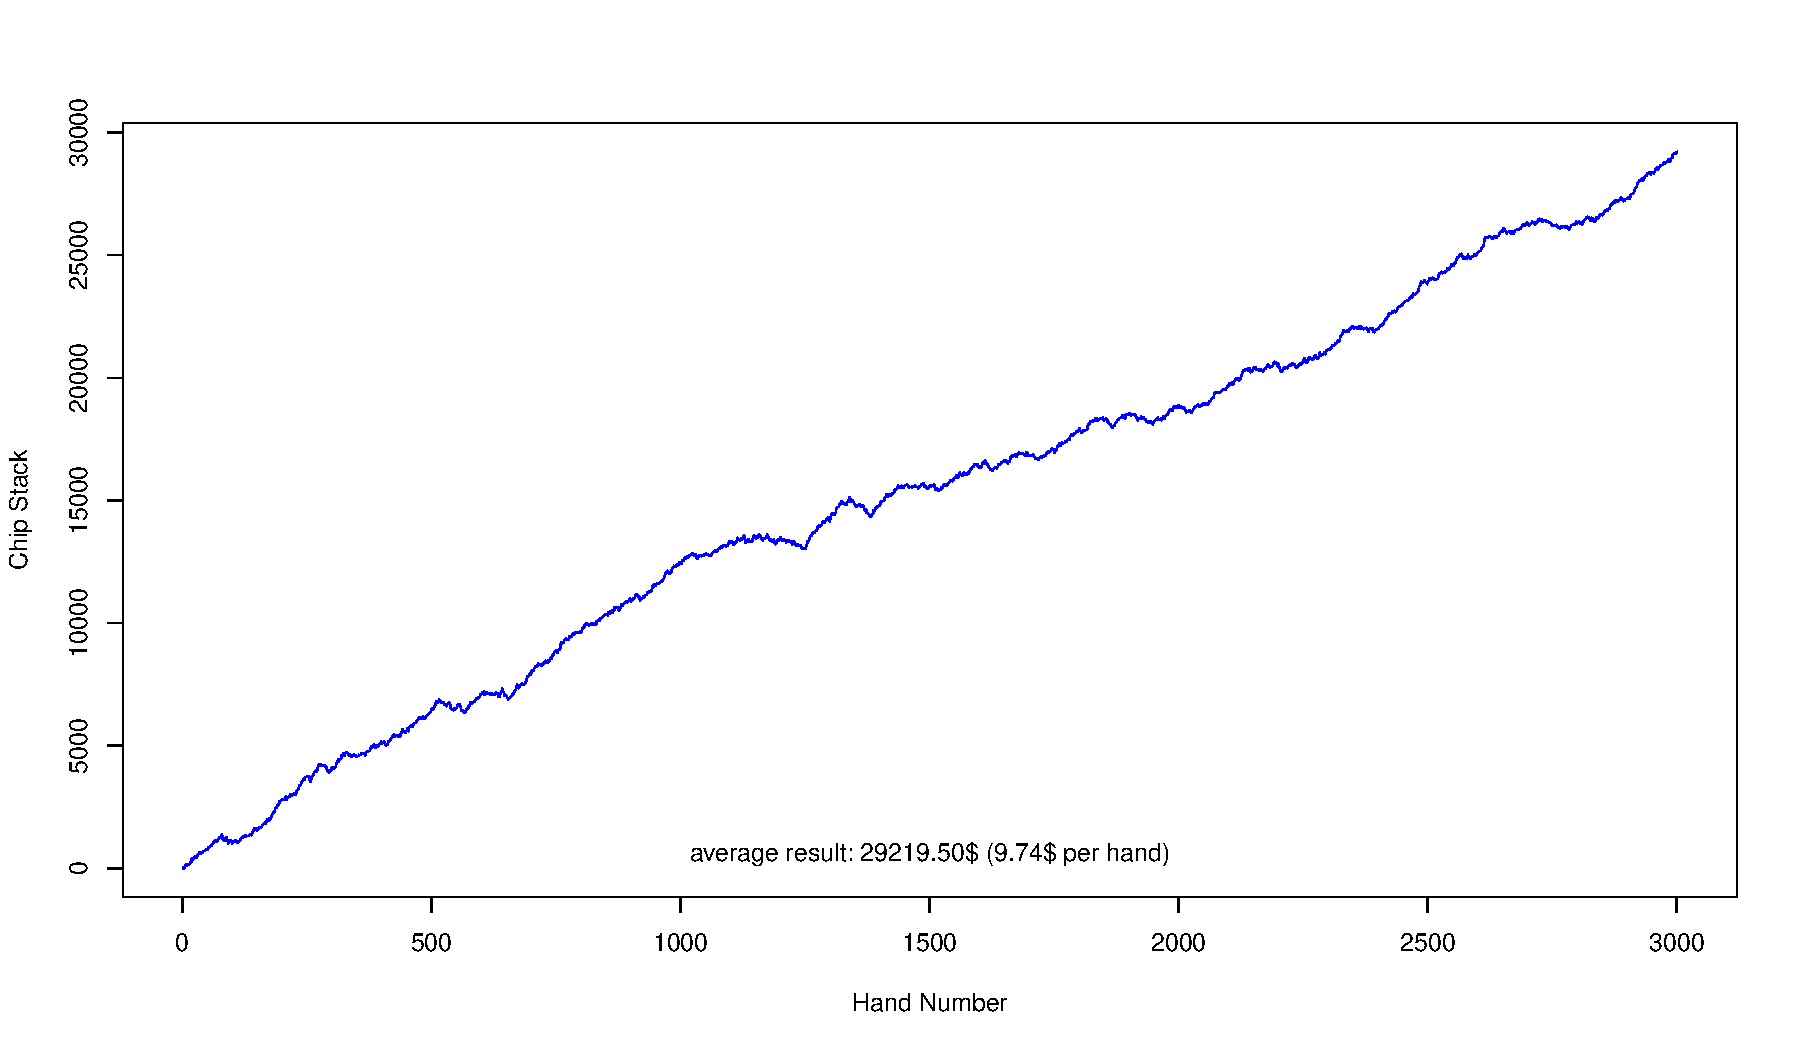
\includegraphics[width=\linewidth]{section06-implementation/figures/matchresults/AveryBot}
\caption{Matchresults: UZHoldem vs. AveryBot}
\label{fig:result-averybot}
\end{figure}

\begin{figure}[!ht]
\centering
\includegraphics[width=\linewidth]{section06-implementation/figures/matchresults/XenBot}
\caption{Matchresults: UZHoldem vs. XenBot}
\label{fig:result-xenbot}
\end{figure}

\begin{figure}[!ht]
\centering
\includegraphics[width=\linewidth]{section06-implementation/figures/matchresults/JamBot}
\caption{Matchresults: UZHoldem vs. JamBot}
\label{fig:result-jambot}
\end{figure}

\begin{figure}[!ht]
\centering
\includegraphics[width=\linewidth]{section06-implementation/figures/matchresults/Random1}
\caption{Matchresults: UZHoldem vs. Random}
\label{fig:result-random}
\end{figure}

\begin{figure}[!ht]
\centering
\includegraphics[width=\linewidth]{section06-implementation/figures/matchresults/AlwaysCall}
\caption{Matchresults: UZHoldem vs. AlwaysCall}
\label{fig:result-alwayscall}
\end{figure}



A two points stick out when investigating these graphs:

\begin{itemize}
	\item Even though a seemly large amount of hands were played, the variance still remains very high. This can be seen especially good in the matches against Jambot and Xenbot. This specific strategy introduces a very large variation, since all-in showdown occur rarely, but influence the result greatly.
	\item Unfortunately, all these graph show a pretty constant slope, without any signs of an performance improvement during the game, as one would probably expect from the adapting opponent model. 
\end{itemize}

\subsection{Results for Opponent Model}
To further investigate the second observation, I reran the opponent model benchmark over the game logs, to measure the improvement of the model during each match:

\subsubsection{Action Prediction}

\begin{figure}[ht!]\centering
\subfigure[Correct Predictions against Always Call]{
\includegraphics[scale=0.265]{section07-results/modelresults/nolimittest2-UZHoldem-AlwaysCall-action-correctly}

}
\subfigure[Quadratic Loss against Always Call]{
\includegraphics[scale=0.265]{section07-results/modelresults/nolimittest2-UZHoldem-AlwaysCall-action-quadratic}

}

\subfigure[Correct Predictions against Always Fold]{
\includegraphics[scale=0.265]{section07-results/modelresults/nolimittest2-UZHoldem-AlwaysFold-action-correctly}

}
\subfigure[Quadratic Loss against Always Fold]{
\includegraphics[scale=0.265]{section07-results/modelresults/nolimittest2-UZHoldem-AlwaysFold-action-quadratic}

}


\end{figure}

\begin{figure}[!ht]\centering
\subfigure[Correct Predictions against AveryBot]{
\includegraphics[scale=0.265]{section07-results/modelresults/nolimittest2-UZHoldem-AveryBot-action-correctly}

}
\subfigure[Quadratic Loss against AveryBot]{
\includegraphics[scale=0.265]{section07-results/modelresults/nolimittest2-UZHoldem-AveryBot-action-quadratic}

}

\end{figure}

\begin{figure}[!ht]\centering

\subfigure[Correct Predictions against JamBot]{
\includegraphics[scale=0.265]{section07-results/modelresults/nolimittest2-UZHoldem-JamBot-action-correctly}

}
\subfigure[Quadratic Loss against JamBot]{
\includegraphics[scale=0.265]{section07-results/modelresults/nolimittest2-UZHoldem-JamBot-action-quadratic}

}

\subfigure[Correct Predictions against XenBot]{
\includegraphics[scale=0.265]{section07-results/modelresults/nolimittest2-UZHoldem-XenBot-action-correctly}

}
\subfigure[Quadratic Loss against XenBot]{
\includegraphics[scale=0.265]{section07-results/modelresults/nolimittest2-UZHoldem-XenBot-action-quadratic}

}
\caption{Action Prediction Performance}


\end{figure}

\newpage

\subsubsection{Hand Prediction}

\begin{figure}[th!]\centering
\subfigure[Mean Error against Always Call]{
\includegraphics[scale=0.265]{section07-results/modelresults/nolimittest2-UZHoldem-AlwaysCall-action-correctly}

}
\subfigure[Quadratic Loss against Always Call]{
\includegraphics[scale=0.265]{section07-results/modelresults/nolimittest2-UZHoldem-AlwaysCall-action-quadratic}

}

\end{figure}

\begin{figure}[!ht]\centering


\subfigure[Mean Error against AveryBot]{
\includegraphics[scale=0.265]{section07-results/modelresults/nolimittest2-UZHoldem-AveryBot-hand-meansquared}

}
\subfigure[Quadratic Loss against AveryBot]{
\includegraphics[scale=0.265]{section07-results/modelresults/nolimittest2-UZHoldem-AveryBot-hand-quadratic}

}


\end{figure}

\begin{figure}[!ht]\centering

\subfigure[Mean Error against XenBot]{
\includegraphics[scale=0.265]{section07-results/modelresults/nolimittest2-UZHoldem-XenBot-hand-meansquared}

}
\subfigure[Quadratic Loss against XenBot]{
\includegraphics[scale=0.265]{section07-results/modelresults/nolimittest2-UZHoldem-XenBot-action-quadratic}

}
\caption{Hand Prediction Performance}


\end{figure}

\newpage
\section{Insights from playing against humans}

To better judge the resulting program in regard to its style of play, I also conducted a round of hands against a human player. This informal experiment should provide a subjective view on how a opponent unaware of the underlining algorithm perceives the resulting play style. To do this, the bot was added to \textit{Poker Academy}, which provided the graphical user interface for the interface. The manual in the appendix explains the necessary steps to play UZHoldem in \textit{Poker Academy}.

\subsection{Pre-Flop Play}

Little surprising, the pre-flop strategy was perceived as very week and transparent. While the algorithm is very defensive versus all-in moves by the opponent, it still re-raises minimal-raises all the way down to a all-in. But if the opponent raises, the program re-raises, and if the player then goes all-in, the program decides to fold. 

\subsection{Post-Flop Play}

Playing after the flop has been dealt was perceived much stronger. While still being somewhat strange, and riddled with exploitable weaknesses, its moves generally make sense. Some observed weaknesses include:

\begin{itemize}
\item Draws are often played extremely aggressive, even re-raising raises.
\item Pairs on the flop are often played very weak, but then suddenly very aggressive on the river, sometimes going all-in, even though the hand didn't improve at all.
\item The hight of a pair seems to not have much of an effect. This results in a overly strong play of weak bottom pairs, calling or raising them all the way to a showdown.
\item The algorithms seems to underestimates the chance of the opponent folding to an all-in move. All-in bets on the flop result in a fold in the vast majority of cases. Still, UZHoldem often bets all-in having the highest pair, obviously assuming this to be a bet that might extract the most money from the opponent. This results in the opponent only calling with absolute winning hands, and folding everything else, resulting in only very small winning but large losses.
\item Generally, the line of actions during a hand is often perceived as random. UZHoldem might bet on the flop, then check on the turn, bet on the river but then fold when faced a raise. Other strange lines include checking on the flop, then calling on the turn and betting all-in on the river as a bluff.
\end{itemize}

Overall, the bot has shown mix performance, which might be comparable to a novice of the game, but unable to derange a more experienced player.
\chapter{Limitations and Future Work}
\label{c:limitations} 

Overall, the resulting implementation has shown acceptable performance. To further improve the strength of this approach there remain a few problems:

\begin{itemize}
\item \textbf{faster and more accurate adaption of the opponent modelling} still remains an unsolved problem. Hoeffding trees are extremely fast and provide acceptable prediction accuracy - but they don't adapt as fast as desired for poker play. Approaches with two models might like proposed by \cite{Ponsen2008}�promise a much faster adaption.

\item \textbf{pre-flop} So far, theres still no approach using game tree search during the game to devise an opponent model based pre-flop strategy. This is especially unfortunate, because pre-flop is the stage of the game, for the lack of community cards, where the opponent model is the most important. Computing performance will stay too slow for full-fledged for some time too come. Therefore, to compute a pre-flop game tree, many more approximations need to be added to the ideas in this thesis to help them remain computationally practical. A lot of possible abstractions for this problem can be found in equilibria-based approaches (like abstracting cards and hands into buckets). 

\item \textbf{bet amounts} UZHoldem uses the betting model of \cite{Gilpin2008}. While generally appropriate, it lacks a variety of characteristics which could be profitable. Since the equilibria-approach of \cite{Gilpin2008}�doesn't adjust to the opponent, the betting model isn't meant to adjust to the opponent either. In reality though, different opponents react different to different bet-sizes. Adding more possible betting-amounts (e.g. also one-third-pot and two-third-pot bets) might advance the exploitation skill of a poker bot. But as these additional actions grow the game tree progressively, a simple adjustment of the current betting sizes might be a more realistic approach. Additionally, as \cite{Gilpin2008} proposed a more systematic automated approach to designing betting abstractions would be preferable.

\item \textbf{extending to multi-player} Like all bots based on Miximax, UZHoldem only plays  heads-up Texas Hold'em. To extend these ideas to multi-player poker, many more approximations need to be added to the ideas in this thesis to help them remain computationally practical.

\item \textbf{more flexible pruning of the game tree}. The current implementation of the game algorithm bases the pruning of the game tree solely on some static properties like three depth and game stage. For No-Limit Poker, a algorithm which takes the stacks-to-blind ratio (how "deep" the players are) into consideration would be more appropriate.
\end{itemize}

%\include{section09-futurework/futurework}
\chapter{Conclusions}
\label{c:conclusion} 

Poker is a challenging domain in artificial intelligence research. It's properties of both chance and imperfect information makes it a good testbed for exploring decision-theory, probabilistic reasoning, risk assessment, and opponent modeling. The challenges found in poker are also present in many other fields related to decision-making, machine learning and behaviour-modelling. To solve these problems, different approaches like expert-systems, simulations and solving linear systems to find equilibria strategies have been explored in the past. 

While computer poker research has progressed tremendously in the past decade, there are still major difficulties hindering the development of a player similar to good human players. One of these challenges is finding a strategy that not only plays strong poker, but also exploits the weaknesses of the current opponent as strong as possible.

The method this thesis focused on consists of two main components: heuristic search for action-selection, and a model of the opponent�s play. This approach was developed by the Computer Poker Lab at the University of Alberta and has shown impressive performance in the past. 

The heuristic search procedure implemented is an example of expectimax search. It takes opponent modeling information and plans a strategy that exploits that information. This thesis presented the ideas behind this approach, and explored the possibility to build an opponent model based on historic data and proven data mining algorithms. 

This means that the learning algorithm of the opponent model isn't only used to update the model, but also to build it - showing a way to solve the problem of bootstrapping the opponent model. Different machine learning algorithms were explored, and a poker playing agent based on a opponent model of two Hoeffding Decision Tree models was implemented.


The opponent modeling information used in the tree search takes the form of observations that the computer player observes in actual game play. These observations include the opponent�s actions, the cards dealt at chance nodes, and the cards revealed by the opponent at showdowns. These observations are added to the model both when building the opponent model by observing historic data and during the game after each hand is played.

To apply the ideas to No-Limit Texas Hold�em, approximations were necessary to keep them practical.  Unlike other work about stochastic search in Texas Hold'em, this thesis focused on the No-Limit variant of the game and adapted techniques from other No-Limit approaches (like $\epsilon$-equilibria calculations) to a tree search based solution. 

No-Limit Texas Hold�em is too large to do a full-depth full-width action-selection search, so the search procedure had to be based on a approximated game tree. These approximations include approximating the possible cards at chance nodes, pruning the game tree based on the opponent action distribution and discretizing the possible continuous betting amounts possible in classes of actions.

The complexity of a game sitation in Texas Hold�em also means that generalization had to be added to the opponent model. With a finite set of attributes, the number of game contexts could be shrunk to a finite amount of different situations an opponent might encounter.

Overall, the resulting computer player implemented using the ideas in this thesis contains minimal expert knowledge. Unlike other approaches like \cite{Schauenberg2006}, no expert knowledge was required to build the initial default opponent model.

Instead of manufacturing a default opponent model with expert knowledge or equilibria calculations, a offline-learner was developed, capable of parsing past games played at the Annual Computer Poker Competition and learning an opponent model based on the decision made by the contestants at these events.

The only expert-knowhow used was the generalization of game contexts in the opponent model, the possible discretized betting amounts and the very simplistic pre-flop strategy of the player.

To evaluate the strength of the implementation, a benchmark tournament with a variety of poker bots was conducted. In this setting, the implementation played against different other agents, ranging from very simple sample enemies (always calling or always folding),  simple strategic bots (either pushing all-in or folding, based on a strategy from poker literature) to commercial bots used to train poker players.

UZHoldem, the name of the implementation, has fared well to acceptable against all opponents. Against humans, it has shown a rather weak performance compared to a regular player, but was fond of the basics of poker.

For further conclusions, the performance of the opponent model in the benchmark tournament was also examined, showing some improvement of the prediction accuracy, but not enough to result in a significant gain in the turnout of actions.



% Appendix
\begin{appendix}
\renewcommand{\chaptermark}[1]{\markboth{\appendixname \ \thechapter.\ #1}{}}
\chapter{Appendix}
\label{a:appendix}

\section{Software Manual}
\label{s:softwaremanual}

The easiest way to play a few hands against UZHoldem is by using Poker Academy. After downloading and installing Poker Academy, the necessary files (found in uzholden-dist.zip) have to be added to the program folder of Poker Academy.


\begin{figure}[!h]\centering
\includegraphics[width=0.65\linewidth]{section-appendix/figures/file-location}
\caption{Target location of the required files}
\label{fig:file-location}
\end{figure}
\begin{figure}[!ht]\centering

\subfigure[The opponent manager is found in the "Window" Menu ]{
\includegraphics[width=0.65\linewidth]{section-appendix/figures/opponent-manager1}

}
\subfigure[Adding a new player]{
\includegraphics[width=0.65\linewidth]{section-appendix/figures/opponent-manager2}
}

\caption{Adding a new player to the opponent manager}
\label{fig:opponent-manager}
\end{figure}

Figure \ref{fig:file-location}�shows the required location of the files in the application package in Mac OS X. On Windows, the steps are similar, when copying all the files into the \texttt{data/bots}� directory.

Although its possible to use UZHoldem with the standard settings, I recommend starting PokerAcademy with a JVM that has 512MB or even 1GB memory available. On Windows, this can by done by starting Poker Academy with the switch \texttt{-JXmx512}, on Mac OSX, this requires changing the \texttt{Info.plist} file in the application package (key \texttt{VMOptions}).

 After copying the files, the only additional step required is adding a new player based on the agent (figure \ref{fig:opponent-manager})

\begin{figure}[!h]\centering
\includegraphics[width=\linewidth]{section-appendix/figures/new-table}
\caption{Creating a new table with two players}
\label{fig:new-ptable}
\end{figure}

As a final step, the opponent can now be placed on a new poker table. 

\end{appendix}

\listoffigures \listoftables

\lstlistoflistings \addcontentsline{toc}{chapter}{List of Listings}

% Bibliography
\bibliographystyle{apalike-url}
\bibliography{section-references/thesisbib}


\end{document}
